%% Author: Saleem Al Dajani, MIT, KAUST. UCB-NE
%% This is the manuscript draft for our paper about LWR MMLC
% draft format
%\documentclass[preprint,12pt]{elsarticle}

% final submission format
%\documentclass[preprint, review, 12pt]{elsarticle}

%% Use the option review to obtain double line spacing
%% \documentclass[preprint,review,12pt]{elsarticle}

%% Use the options 1p,twocolumn; 3p; 3p,twocolumn; 5p; or 5p,twocolumn
%% for a journal layout:
%% \documentclass[final,1p,times]{elsarticle}
%% \documentclass[final,1p,times,twocolumn]{elsarticle}
\PassOptionsToPackage{numbers,sort&compress}{natbib}
\documentclass[final,3p,times]{elsarticle}
%\documentclass[final,3p,times,twocolumn]{elsarticle}
%% \documentclass[final,5p,times]{elsarticle}
%% \documentclass[final,5p,times,twocolumn]{elsarticle}
\usepackage{natbib}
%% The graphicx package provides the includegraphics command.
\usepackage{graphicx}
%% The amssymb package provides various useful mathematical symbols
\usepackage{amssymb}
\usepackage{amsmath} 
%% The amsthm package provides extended theorem environments
%% \usepackage{amsthm}
\usepackage{fancyhdr}
\usepackage{hyperref}
\usepackage{caption}
\usepackage{subcaption}
\usepackage{wrapfig}
\usepackage{lscape}
\usepackage{rotating}
\usepackage{epstopdf}
\usepackage{comment}
\usepackage{xurl}
%\usepackage[figuresfirst,nomarkers,nolists,figuresonly,noheads]{endfloat}
% Tell endfloat to handle sidewaysfigure the same as figure
%\DeclareDelayedFloatFlavor{sidewaysfigure}{figure}
\makeatletter
\def\NAT@def@citea{\def\@citea{\NAT@separator}}
\makeatother
\hypersetup{
colorlinks,
citecolor=blue,
filecolor=blue,
linkcolor=blue,
urlcolor=blue
}

%% The lineno packages adds line numbers. Start line numbering with
%% \begin{linenumbers}, end it with \end{linenumbers}. Or switch it on
%% for the whole article with \linenumbers after \end{frontmatter}.
\usepackage{lineno}

%% natbib.sty is loaded by default. However, natbib options can be
%% provided with \biboptions{...} command. Following options are
%% valid:

%%   round  -  round parentheses are used (default)
%%   square -  square brackets are used   [option]
%%   curly  -  curly braces are used      {option}
%%   angle  -  angle brackets are used    <option>
%%   semicolon  -  multiple citations separated by semi-colon
%%   colon  - same as semicolon, an earlier confusion
%%   comma  -  separated by comma
%%   numbers-  selects numerical citations
%%   super  -  numerical citations as superscripts
%%   sort   -  sorts multiple citations according to order in ref. list
%%   sort&compress   -  like sort, but also compresses numerical citations
%%   compress - compresses without sorting
%%
%% \biboptions{comma,round}

% \biboptions{}

\usepackage{xcolor}
\usepackage{soul}
\DeclareRobustCommand{\upd}[1]{{\sethlcolor{yellow}\hl{To be updated: #1}}}
\usepackage{booktabs}
\usepackage{placeins}

\journal{Scripta Materialia}

\begin{document}
\begin{frontmatter}

\title
{
\textbf
{
First principles evidence of stiffening \\ during spinodal decomposition in FeCr
}
}

\date
{\today}
\rhead{\today}

\author[1]{Saleem A. Al Dajani}
\author[1]{Michael P. Short}

\address{
Department of Nuclear Science and Engineering \\
Massachusetts Institute of Technology\\
77 Massachusetts Avenue \\
Cambridge, MA 02139}

\address[1]
{
Corresponding Author: \href{mailto:sdajani@mit.edu}{\texttt{sdajani@mit.edu}}
}

\begin{abstract}

We explain stiffening during spinodal decomposition in \emph{bcc} $\delta$-ferrite previously observed in cast austenitic stainless steels by combining experimental measurements with first-principles simulations of \emph{bcc} Fe$_{1-x}$Cr$_x$. Quantum elastodynamic calculations predict surface acoustic wave (SAW) peak splitting arising from elastic stiffening of $\delta$-ferrite during spinodal decomposition. Classical first-principles elastodynamics also quantitatively calculate Rayleigh SAW peak splitting arising from spinodal stiffening as a non-destructive indicator of embrittlement, consistent with experiment. More broadly, similar SAW-based stiffening signatures may prove useful for detecting other embrittlement mechanisms in structural alloys.

\end{abstract}

\begin{keyword}
Stainless steel \sep 
binary alloy \sep
iron-chrome \sep
spinodal decomposition
\sep
surface acoustic wave \sep 
\emph{Ab initio} calculation
\sep
stiffening
\sep
embrittlement
\sep
thermal diffusivity
\sep
$\delta$--ferrite
\sep
quantum elastodynamics (QED)
%% keywords here, in the form: keyword \sep keyword

%% MSC codes here, in the form: \MSC code \sep code
%% or \MSC[2008] code \sep code (2000 is the default)

\end{keyword}

\end{frontmatter}

\textbf{Highlights}

\begin{itemize}
\item Ab initio simulations predict stiffening during spinodal decomposition in $\delta$--ferrite
\item Composition-dependent elasticity maps to surface acoustic wave frequency shifts
\item Theory and experiment agree: stiffening non-destructively indicates embrittlement
\end{itemize}


\section{Introduction and Background}
Recent structure--property studies have linked spinodal decomposition to stiffening of \textit{bcc} $\delta$--ferrite in cast austenitic stainless steels (CASS), and have shown that this stiffening can be detected through picosecond ultrasonic surface acoustic wave (SAW) peak splitting \cite{al2023detecting, al2020detecting,al2020non}.
This paper establishes a quantitative theoretical foundation for predicting that SAW signature from first principles by combining elastodynamics with density functional theory (DFT) to connect composition, elastic response, and Rayleigh-wave observables.

For high--melting-point metals (including \textit{bcc} $\delta$--ferrite), elasticity is often closely tied to plastic response: dislocation energetics are largely stored in the Hookean lattice outside the dislocation core, and thermally activated processes during deformation can modify elastic properties \cite{pugh1954xcii}.
More broadly, cohesive properties quantified by lattice elasticity correlate with melting point through their shared dependence on interatomic bonding and electronic structure \cite{chang1966correlation,fine1984elastic, korzhavyi2009electronic, razumovskiy2011first, hosemann2018materials}.
In ferromagnetic Fe--Cr alloys, these quantities vary strongly with concentration \cite{korzhavyi2009electronic}, and the experimentally observed SAW peak splitting upon spinodal decomposition is consistent with an anomalous concentration dependence of elastic constants associated with electronic-structure effects (including Fermi-surface topology changes \cite{razumovskiy2011first}).

During spinodal decomposition of \textit{bcc} $\delta$--ferrite, chromium partitioning produces Fe-rich $\alpha$ and Cr-rich $\alpha'$ regions whose differing compositions imply differing stiffness. As a result, elastic stiffening can serve as a mechanistically grounded proxy for embrittlement in stainless steels undergoing thermal and/or irradiation-assisted aging \cite{du2017facile, sdajani2019cassspinodal,al2020non, hofmann2019transient, al2020detecting,byun2016thermal,lach2020precipitation}.
Because the Rayleigh SAW frequency depends directly on elastic moduli, picosecond ultrasonic pump--probe spectroscopy provides a direct, non-destructive route to infer stiffness changes and therefore track the progression toward embrittlement \cite{hofmann2019transient}.

Motivated by these links, we develop a thermodynamics-to-observable workflow for \textit{bcc} Fe$_{1-x}$Cr$_x$ as a model for $\delta$--ferrite: (i) we identify spinodally unstable composition windows using the curvature of the demixing free energy, (ii) we quantify the composition dependence of cubic elastic constants from DFT, and (iii) we map these elastic inputs into Rayleigh SAW frequency ranges using elastodynamic constraints relevant to picosecond ultrasonics. Finally, we separate a solid-solution trend $f_{\mathrm{SAW}}(x_{\mathrm{Cr}})$ from an evolution trend $f_{\mathrm{SAW}}(\phi)$ parameterized by the spinodal conversion fraction $\phi$ from our earlier atomistic simulations of decomposed Fe--Cr \cite{al2023detecting}, enabling direct interpretation of SAW peak shifts and splitting in terms of composition and decomposition state.


\section{Methods}

\subsection{Elastodynamic Methods}
Elastic waves in each homogeneous alloy obey the elastodynamic wave equation \cite{du2017facile}:

\begin{equation}
    \rho \frac{\partial^2 u_i}{\partial t^2} = C_{ijkl} \frac{\partial^2 u_k}{\partial x_j \partial x_l}
    \label{eqn:ewe}
\end{equation}

where $C_{ijkl}$ are fourth-order stiffness tensor entries indexed by $i,j,k,l=1,2,3$, $\rho$ is density, and $u$ is the displacement field. On its own, Eq.~\ref{eqn:ewe} describes bulk waves in an unbounded medium. The SAW measured by transient grating spectroscopy (TGS), however, is a Rayleigh wave guided by the free surface. Because crystal orientation is not resolved in the present calculations, we solve this surface problem for the isotropic Voigt--Reuss--Hill (VRH) average of each elastic tensor (Sec.~\ref{sec:analysis}). The Rayleigh velocity is then $v_R = v_s\sqrt{q}$, where $q$ is the root in $0<q<1$ of
\begin{equation}
q^3 - 8q^2 + (24-16\beta)q - 16(1-\beta) = 0, \qquad \beta = v_s^2/v_p^2,
\label{eqn:rayleigh}
\end{equation}
with $v_s=\sqrt{G/\rho}=\sqrt{E/[2(1+\nu)\rho]}$ and $v_p=\sqrt{(B+4G/3)/\rho}$. The SAW frequency is $f_{\mathrm{SAW}} = v_R/\lambda$ with $\lambda = 6.4\,\mu$m, the grating period of our TGS measurements \cite{al2023detecting}. Density is interpolated linearly between \textit{bcc} Fe (7870 kg m$^{-3}$) and Cr (7200 kg m$^{-3}$). The boundary conditions, the calculation of the elastic tensor, and the full text of Sections 2--3 before condensation are given in SM Section S11.


\subsection{DFT Methods}
In order to model the BCC Fe--Cr $\delta$--ferrite solid solution, the special quasirandom structure (SQS) methodology was employed \cite{VandeWalleLiu2013}, with SQS supercells generated by the \texttt{mcsqs} software package within the Alloy Theoretic Automated Toolkit (ATAT).
The Vienna \textit{ab initio} Simulation Package (VASP) \cite{kresse1996vasp} was used to perform the density functional theory (DFT) total energy calculations, which were used to derive the elastic properties as well as the enthalpy of mixing.
Spin--polarized DFT calculations were performed on 40--atom SQS supercells employing $\Gamma$--point sampling of reciprocal space along with a 500 eV planewave cutoff energy, with the Projector--Augmented Wave (PAW) method \cite{kresse1999paw} and the Perdew--Burke--Ernzerhof parameterization \cite{pbe1996} of the Generalized Gradient Approximation (GGA). Calculations were performed at $x_{\mathrm{Cr}} = 0$, 0.20, 0.50, 0.95, and 1.00. The self-consistent field procedure (Fig.~\ref{fig:SCF-loop}) and the independent Quantum ESPRESSO calculations are described in SM Sections S11 and S3.


\subsection{Atomistic simulations of decomposed Fe--Cr}
\label{sec:md}
The spinodal conversion fraction $\phi$ and the corresponding elastic moduli are taken from our earlier atomistic study \cite{al2023detecting} (Sec.~3.7 and Fig.~8 therein). These simulations were performed with LAMMPS \cite{plimpton1995}, not VASP, and include no electronic structure. A $50\times50\times50$ \textit{bcc} cell of 250,000 atoms with equiatomic composition was populated randomly and phase-separated by Monte Carlo atom swaps; intermediate states were produced by converting a fraction of the Fe atoms to Cr and the same fraction of Cr atoms to Fe. The elastic constants of each state were calculated by finite deformation with the Fe--Cr two-band embedded-atom-method (EAM) potential of Bonny \textit{et al.} \cite{bonny2011iron}, for ten alloys generated with different random seeds. On this scale, $\phi=0.5$ is the random homogeneous alloy and $\phi=1$ the fully separated structure. Relaxed cell volumes were not retained, so the density is held at the equiatomic value of 7535 kg m$^{-3}$.

To extend the decomposition series beyond the equiatomic alloy, we repeated the full procedure at twelve compositions from $x_{\mathrm{Cr}}=0.05$ to 0.95 in a $25\times25\times25$ cell (31,250 atoms), preserving the composition, and computed random alloys across composition with the same stiffness procedure and potential. Five alloys with different random seeds were generated per composition, and the figures show their mean and standard deviation. As a check, the same small-cell procedure at 50/50 reproduces the bulk modulus of the original series to within 0.2 GPa at every $\phi$ (SM Fig.~\ref{fig:S_md_validation}). All LAMMPS inputs, random seeds, and potential files are provided in the accompanying repository.

\subsection{Analysis of DFT Results}
\label{sec:analysis}
With the elastic tensor obtained from quantum mechanical calculations, the isotropic VRH moduli used in Eq.~\ref{eqn:rayleigh} are calculated as follows; the same moduli enter the Pugh embrittlement criterion and the thermal estimates reported in the Supplementary Material.

\begin{equation}
\begin{aligned}
C' &= \frac{C_{11}-C_{12}}{2},
&\quad
B &= \frac{C_{11}+2C_{12}}{3}, \\
C_{11} &= \frac{3B+4C'}{3},
&\quad
C_{12} &= C_{11}-2C', \\
G_V &= \frac{C_{11}-C_{12}+3C_{44}}{5},
&\quad
G_R &= \frac{5(C_{11}-C_{12})C_{44}}{4C_{44}+3(C_{11}-C_{12})}, \\
G &= \frac{G_V+G_R}{2},
&\quad
E &= \frac{9BG}{3B+G},
&\quad
\nu &= \frac{3B-E}{6B}.
\end{aligned}
\label{eqn:moduli}
\end{equation}

Equation~\ref{eqn:moduli} gives the cubic forms used for the literature tensors. For the DFT points, $B$ and $G$ are VRH averages of the full calculated tensor, because the SQS cells are not exactly cubic. All figures are generated from tabulated inputs by scripts provided in the accompanying repository (see Data Availability).


\section{Results}

\subsection{Spinodal stability from demixing free-energy curvature}

The local stability of a binary solid solution is governed by the curvature of its free energy of mixing with respect to composition. Where $\partial^2 \Delta G_{\mathrm{mix}}/\partial x_{\mathrm{Cr}}^2 < 0$, infinitesimal composition fluctuations lower the free energy, and demixing proceeds spontaneously without the need for nucleation barriers. Figure~\ref{fig:free_energy} is evaluated at 298.15 K from the concentration-dependent interaction models that Levesque \textit{et al.} fitted to PWSCF--PAW and SIESTA--NC calculations \cite{levesque2011simple}, $\Omega(x)=(x-a)(bx^2+cx+d)$, together with the ideal configurational entropy $S_{\mathrm{mix}}$. Following the sign convention of that model, we plot the demixing free energy
\begin{equation}
\Delta G_{\mathrm{demix}} = \Omega(x)\,x(1-x) + T S_{\mathrm{mix}} = -\Delta G_{\mathrm{mix}}.
\label{eqn:demix}
\end{equation}
The spinodal criterion $\partial^2 \Delta G_{\mathrm{mix}}/\partial x_{\mathrm{Cr}}^2 < 0$ therefore appears as \emph{positive} curvature, $\partial^2 \Delta G_{\mathrm{demix}}/\partial x_{\mathrm{Cr}}^2 > 0$, in Fig.~\ref{fig:free_energy}b, where three-point numerical second differences fall on the exact curve.

% --- FIGURE: free energy + curvature ---
\begin{figure}[!h]
\centering
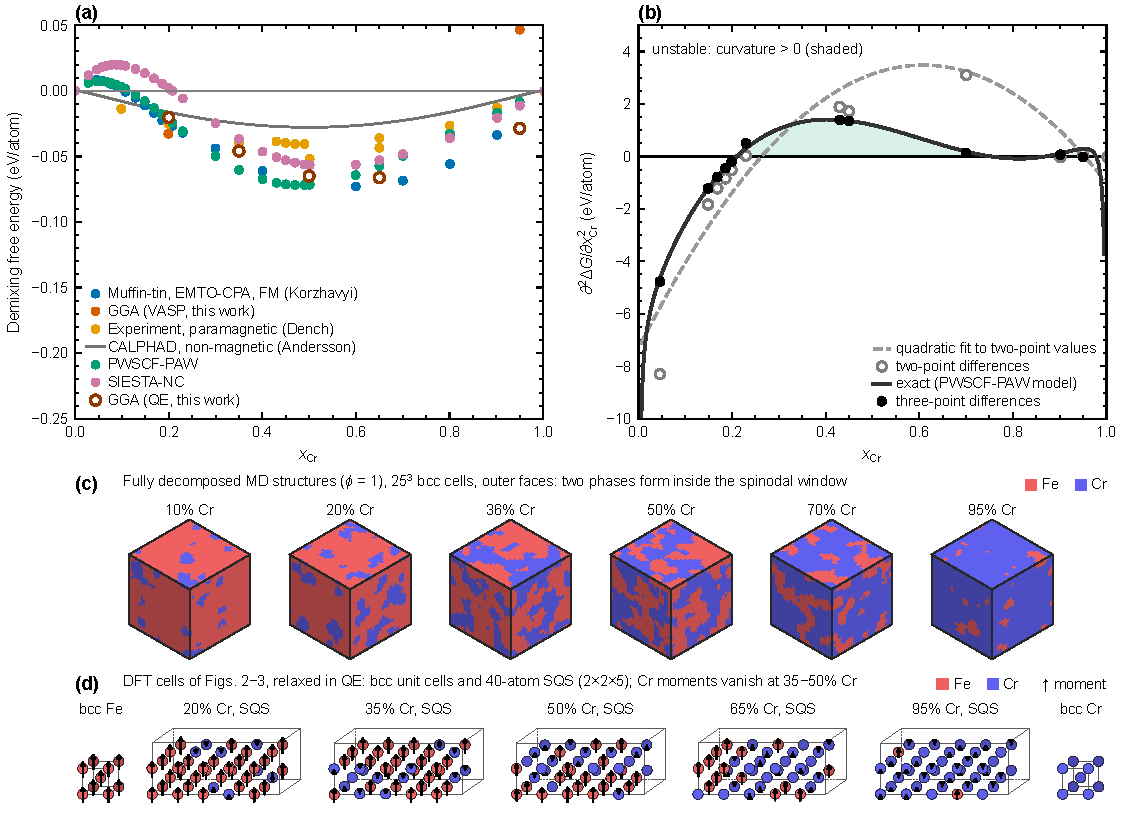
\includegraphics[width=\linewidth]{figures/kdense_scripta/with_strips/fig1_free_energy_qe_entropyfix_strip_cube_dft.pdf}
\caption{(a) Demixing free energy $\Delta G_{\mathrm{demix}} = -\Delta G_{\mathrm{mix}}$ (Eq.~\ref{eqn:demix}) versus chromium composition $x_{\mathrm{Cr}}$ at 298.15 K: muffin-tin (EMTO-CPA, ferromagnetic) enthalpies of Korzhavyi \textit{et al.} \cite{korzhavyi2009electronic}, present GGA calculations with VASP (filled) and Quantum ESPRESSO (40-atom SQS, references FM Fe and AFM Cr; open circles at the PBE-relaxed lattice parameter, open diamonds at the room-temperature experimental lattice parameter with the references at theirs, which changes $\Delta G_{\mathrm{demix}}$ by at most 10 meV/atom), calorimetric enthalpies of Dench \cite{dench1963adiabatic} (measured near 1600 K relative to paramagnetic Fe and Cr), the CALPHAD bcc description of Andersson and Sundman \cite{andersson1987thermodynamic} (non-magnetic part, line), and the PWSCF--PAW and SIESTA--NC interaction models of Levesque \textit{et al.} \cite{levesque2011simple}. All series include the ideal configurational entropy as in Eq.~\ref{eqn:demix}; the measured vibrational entropy of mixing, about $0.2\,k_{\mathrm{B}}$/atom \cite{fultz1995phonon}, would change $\Delta G_{\mathrm{demix}}$ by at most 5 meV/atom at this temperature. (b) Curvature of the PWSCF--PAW demixing free energy. Solid line: exact analytic second derivative of the model. Filled circles: three-point second differences of its tabulated values on the non-uniform composition grid. Open circles: two-point second differences of the same values, with a quadratic least-squares fit (dashed). Shading marks positive demixing curvature, i.e., negative mixing curvature, which identifies spinodally unstable compositions. (c) Fully decomposed ($\phi=1$) MD structures, viewed as whole $25^3$ \textit{bcc} cells (three outer faces, corner sublattice; Sec.~\ref{sec:md}) at the indicated Cr contents; red, Fe; blue, Cr. Inside the spinodal window the alloy separates into interpenetrating Fe-rich $\alpha$ and Cr-rich $\alpha'$ domains, whereas at the dilute ends the minority element forms only isolated clusters. (d) The DFT cells: \textit{bcc} unit cells of Fe and Cr and 40-atom SQS ($2\times2\times5$ conventional cells), relaxed in Quantum ESPRESSO, with their local magnetic moments (arrows; red, Fe; blue, Cr). The Cr moments, antiparallel to Fe at 20\% Cr, vanish between 35 and 50\% Cr.}
\label{fig:free_energy}
\end{figure}

Figure~\ref{fig:free_energy}b shows that the homogeneous alloy is unstable for $0.21 \lesssim x_{\mathrm{Cr}} \lesssim 0.75$ in the PWSCF--PAW model (with a second, narrow window at $0.87$--$0.98$); the SIESTA--NC model gives $0.25 \lesssim x_{\mathrm{Cr}} \lesssim 0.99$. Both windows contain the Fe--36Cr alloy in which spinodal decomposition was recently detected through TGS stiffening \cite{rae2026tgs}. At the 748 K aging temperature the CALPHAD assessment of Xiong \textit{et al.} places the chemical spinodal at $x_{\mathrm{Cr}}\approx0.30$--0.71 \cite{xiong2011improved}, so Fe--36Cr lies inside it, close to its Fe-rich edge. Within these windows, elastic and acoustic properties cannot be interpreted assuming a homogeneous solid solution. Instead, any observable elastic response must be understood as emerging from a system that is intrinsically driven toward compositional modulation, providing the foundation for linking free-energy curvature to stiffness evolution and ultimately to ultrasonic observables.

\subsection{Elastic stiffening and elastodynamic mapping to Rayleigh SAW observables}

% --- FIGURE: elasticity + elastodynamics ---
\begin{figure}[!h]
\centering
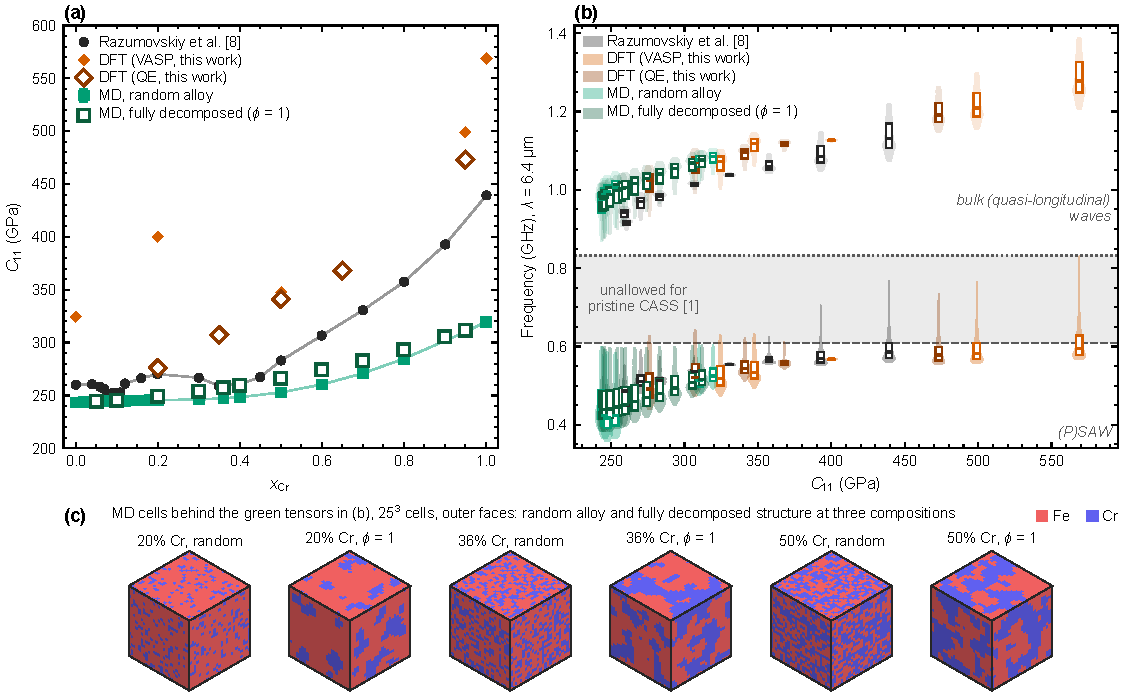
\includegraphics[width=\linewidth]{figures/kdense_scripta/with_strips/fig2_elastic_mapping_orientation_violin_bulk_mddecomp_qe_strip_cube.pdf}
\caption{(a) $C_{11}$ of \textit{bcc} Fe$_{1-x}$Cr$_x$: literature calculations of Razumovskiy \textit{et al.} \cite{razumovskiy2011first} (black circles; reconstructed from digitized $C'$, $C_{44}$, and $B$), present DFT calculations on 40-atom SQS with VASP (filled red diamonds) and Quantum ESPRESSO at the PBE-relaxed lattice parameter (open diamonds) and at the experimental lattice parameter (filled blue diamonds; 5--50 and 95\% Cr) (SM S3), MD (EAM) random alloys (green squares; mean $\pm$ standard deviation of ten alloys at the DFT compositions and three elsewhere; Sec.~\ref{sec:md}), and fully decomposed MD structures ($\phi=1$, open squares; $25^3$ cells). (b) Orientation-resolved acoustic frequencies at $\lambda=6.4\,\mu$m, plotted at the $C_{11}$ of each tensor in (a). For each tensor, 10{,}000 random grain orientations were computed with the surface Green's-function method of Du and Zhao \cite{du2017facile}, as in Ref.~\cite{al2023detecting}. Lower violins: (pseudo-)SAW frequencies (pseudo-SAW retained when its intensity is at least $2\times10^{-3}$ of the SAW). Upper violins: quasi-longitudinal bulk waves along the same propagation directions. Boxes mark the interquartile range and median. The shaded band is the elastodynamically unallowed range of pristine 304-type CASS \cite{al2023detecting}, from its maximum (pseudo-)SAW frequency (0.609 GHz, dashed) to its bulk-wave frequency (0.833 GHz, dotted). (c) The MD cells behind the green tensors, viewed as whole $25^3$ cells (three outer faces): random alloy and fully decomposed structure at $x_{\mathrm{Cr}}=0.20$, 0.36, and 0.50 (red, Fe; blue, Cr). Panel (b) shows both QE sets, in the colours of (a).}
\label{fig:elastic_elastodynamics}
\end{figure}

To connect thermodynamic instability to experimentally measurable quantities, we compute the cubic elastic tensor across $x_{\mathrm{Cr}}$ and propagate these elastic inputs through the surface boundary-value problem of Sec.~2.1. Although $f_{\mathrm{SAW}}$ depends on the full tensor through $B$ and $G$, we use the longitudinal stiffness $C_{11}$ as a compact index of composition-dependent stiffening (Fig.~\ref{fig:elastic_elastodynamics}a). The fully decomposed MD structures are stiffer than the random alloy at every composition, most strongly at intermediate compositions (e.g., 257.4 versus 247.3 GPa at $x_{\mathrm{Cr}}=0.36$). The present DFT tensors are systematically stiffer than the reference data (e.g., $C_{11}=324$ versus 260 GPa for \textit{bcc} Fe), so we interpret relative trends rather than absolute frequencies; Quantum ESPRESSO calculations at the experimental lattice parameter follow the literature between 30 and 50\% Cr ($C_{11}$ within 11 GPa).

In our earlier study, elastodynamic calculations for pristine CASS over randomly sampled grain orientations defined an ``unallowed'' frequency range, above the highest (pseudo-)SAW frequency and below the bulk-wave frequency, in which no surface mode of the pristine material exists; (P)SAW peaks observed there after aging were attributed to stiffened $\delta$-ferrite \cite{al2023detecting}. Figure~\ref{fig:elastic_elastodynamics}b repeats that calculation for every Fe--Cr tensor. In the (P)SAW branch, no literature tensor up to $x_{\mathrm{Cr}}=0.7$ and none of the MD tensors reaches it, even after full decomposition. Only the stiffest tensors enter it: Cr-rich literature alloys and the present DFT tensors (30\% and 46\% of grains at $x_{\mathrm{Cr}}=0.95$ and 1.0). Frequencies in this range therefore indicate stiffness beyond that of a homogeneous solid solution of $\delta$-ferrite or Fe--36Cr composition, consistent with the stiffer Cr-rich $\alpha'$ regions formed by spinodal decomposition (Fig.~\ref{fig:fsaw_combined}a) and with the peak splitting observed after aging \cite{al2023detecting}. Decomposition stiffens mainly the tetragonal shear modulus $C'$ (by 17--29\% for Fe--36Cr, through the Cr-rich $\alpha'$ phase), which makes weak high-velocity pseudo-SAWs above 665~MHz three to five times more frequent, as in the measured tail (SM Section S9). At the electronic level, the stiffer $C'$ of $\alpha'$ follows the filling of the \textit{bcc} $d$ band \cite{soderlind1993theory}, and the electronic topological transition at $x_c\approx0.08$ (SM Section S6) sets the anomalous moduli of the Fe-rich $\alpha$ phase.

The same shear stiffening links the acoustic signal to embrittlement: decomposition raises $G$ (+11\% for MD Fe--36Cr) while leaving $K$ nearly unchanged ($-1.2\%$), so Pugh's ratio $K/G$ falls by 11\% \cite{pugh1954xcii} in step with the SAW shift, while the cleavage resistance, which scales with $K$, stays fixed. Stiffening therefore shifts the balance from plastic flow towards cleavage, as in the Charpy energies of Ref.~\cite{al2023detecting}, which fall from 88.5~J to 14--24~J for CF8 aged 10{,}000~h at 330--400~$^\circ$C as the SAW splitting grows from 12 to 128--229~MHz (SM Section S9). Within the spinodally unstable composition window, elastic stiffening therefore translates into measurable acoustic signatures, enabling stiffness changes to be inferred non-destructively.

\subsection{Separating composition trends from spinodal conversion trends}

While elastic constants vary with chromium concentration even in a homogeneous solid solution, spinodal decomposition introduces an additional, time-dependent microstructural evolution. We therefore report two complementary relationships that isolate these contributions within a unified elastodynamic framework.

% --- FIGURE: fSAW vs xCr and vs phi ---
\begin{figure}[!h]
\centering
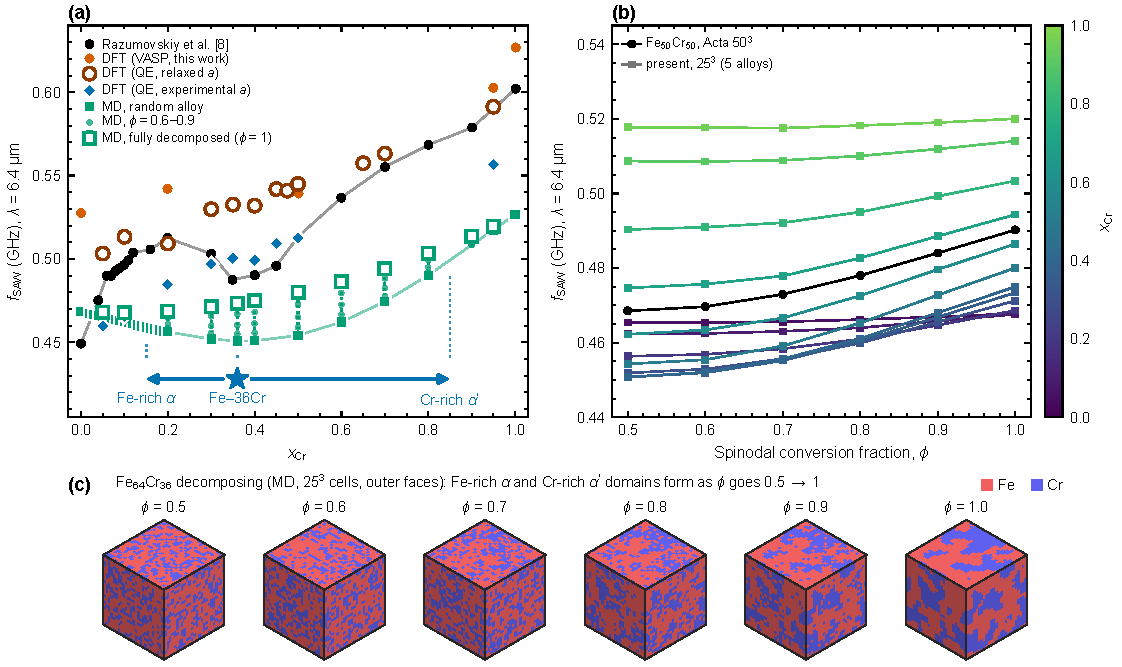
\includegraphics[width=\linewidth]{figures/kdense_scripta/with_strips/fig3_fsaw_mddecomp_6p4um_qe_allx_strip_cube.pdf}
\caption{(a) Rayleigh SAW frequency $f_{\mathrm{SAW}}$ versus chromium composition $x_{\mathrm{Cr}}$ ($\lambda=6.4\,\mu$m) for the literature (black), present DFT (VASP, filled red; Quantum ESPRESSO at the PBE-relaxed lattice parameter, open circles, and at the experimental lattice parameter, filled blue diamonds), and MD random-alloy (green) data of Fig.~\ref{fig:elastic_elastodynamics}. At each MD composition, small dots ($\phi=0.6$--0.9) and an open square ($\phi=1$) show the frequency of the decomposing structure, each series anchored to the random-alloy value at that composition, so the ladder height is the stiffening on decomposition (as in b). Below the data, the star marks Fe--36Cr \cite{rae2026tgs} and the arrows indicate schematically the partitioning toward Fe-rich $\alpha$ and Cr-rich $\alpha'$ during spinodal decomposition; dotted lines rise from each composition toward the data. Arrow endpoints are illustrative, not measured phase compositions. (b) $f_{\mathrm{SAW}}$ versus spinodal conversion fraction $\phi$ from the MD (EAM) decomposition simulations (Sec.~\ref{sec:md}): all twelve compositions, $x_{\mathrm{Cr}}=0.05$--0.95, from the present $25^3$-cell calculations (squares, coloured by $x_{\mathrm{Cr}}$; Fe$_{50}$Cr$_{50}$ in this cell is the check of the original series), and equiatomic Fe$_{50}$Cr$_{50}$ from Ref.~\cite{al2023detecting} (black circles, $50^3$ cell, fixed density 7535 kg m$^{-3}$). $\phi=0.5$ is the random alloy and $\phi=1$ the fully separated structure. (c) The whole $25^3$ MD cell of Fe$_{64}$Cr$_{36}$ (three outer faces) from $\phi=0.5$ to 1.0 (red, Fe; blue, Cr): Fe-rich $\alpha$ and Cr-rich $\alpha'$ domains form and coarsen as $\phi$ increases; these are the structures whose frequencies are plotted in (b). All $25^3$-cell values are means over five MD alloys (random seeds); their $\pm1$ s.d. error bars (at most 0.5 MHz) are smaller than the symbols.}
\label{fig:fsaw_combined}
\end{figure}

Figure~\ref{fig:fsaw_combined}a shows how chromium partitioning produces stiffening. The Fe--36Cr composition lies near a local minimum of the homogeneous $f_{\mathrm{SAW}}(x_{\mathrm{Cr}})$ curve. Spinodal decomposition moves material toward Fe-rich $\alpha$ and Cr-rich $\alpha'$ compositions (arrows); in both directions the homogeneous-alloy frequency increases. The MD random alloys, an independent classical model, also show a frequency minimum, at $x_{\mathrm{Cr}}\approx0.36$--0.40, even though their $C_{11}$ increases monotonically: the minimum comes from the shear moduli, which control the Rayleigh velocity. $C_{11}$ is therefore a convenient index of stiffening, but the SAW response is governed by shear stiffness.

Figure~\ref{fig:fsaw_combined}b isolates the effect of decomposition at fixed overall composition. For Fe$_{50}$Cr$_{50}$ in the MD (EAM) simulations, $f_{\mathrm{SAW}}$ increases monotonically from 0.469 GHz for the random alloy ($\phi=0.5$) to 0.490 GHz for the fully separated structure ($\phi=1$), an increase of about 4.6\%. Repeating the decomposition at twelve compositions gives frequency increases that are nearly symmetric about the equiatomic composition, from 0.5\% at $x_{\mathrm{Cr}}=0.05$ to 5.0\% at Fe--36Cr and 5.7\% at $x_{\mathrm{Cr}}=0.50$. Stiffening on decomposition is therefore largest within the spinodally unstable window of Fig.~\ref{fig:free_energy}b and nearly vanishes for the dilute alloys at either end; the fully separated state is an idealized limit, so these values bound the stiffening from above. Together, $f_{\mathrm{SAW}}(x_{\mathrm{Cr}})$ captures the baseline elastic response of a homogeneous alloy, and $f_{\mathrm{SAW}}(\phi)$ reflects the additional stiffening associated with progressive spinodal conversion.


\section{Discussion}

Taken together, the results establish a closed thermodynamics-to-observable pathway for interpreting picosecond ultrasonic measurements in $\delta$--ferrite--containing stainless steels. The free-energy curvature criterion identifies the composition window in which the homogeneous solid solution is intrinsically unstable, defining the regime where elastic and acoustic properties must reflect ongoing or incipient spinodal decomposition rather than equilibrium alloy behavior.

Within this thermodynamically unstable regime, first-principles elasticity reveals systematic stiffening trends that are propagated through elastodynamic constraints into Rayleigh SAW frequency shifts. The direct mapping between elastic constants and SAW observables provides a quantitative basis for interpreting peak shifts and splitting as signatures of stiffness evolution, rather than purely phenomenological indicators.

Crucially, separating the solid-solution trend $f_{\mathrm{SAW}}(x_{\mathrm{Cr}})$ from the spinodal conversion trend $f_{\mathrm{SAW}}(\phi)$ resolves a key ambiguity in experimental interpretation. While composition alone can shift SAW frequencies, progressive spinodal decomposition introduces additional stiffening that cannot be captured by composition-dependent elasticity alone. The combined framework therefore enables SAW peak splitting to be interpreted as a mechanistically grounded indicator of microstructural evolution toward embrittlement, rather than as a purely compositional effect.

Consistent with experiment, the models reproduce the sign and composition dependence of the stiffening, although not its full size: aging raises the mean second TGS peak of CASS by 90--220~MHz (Table~3 of Ref.~\cite{al2023detecting}), whereas full decomposition raises the frequencies of binary Fe--Cr by 5--8\%. The models omit the Ni, Mn, Si and (in CF8M) Mo of CASS ferrite and its G-phase and carbide precipitates \cite{byun2016thermal,lach2020precipitation}. Each 100--140~$\mu$m TGS spot also samples several ferrite and austenite grains, so the mean second peak mixes stiffening with which grain, phase or mode is detected, including the weak high-velocity pseudo-SAWs that decomposition makes more frequent, whereas we count modes rather than detected amplitudes. Finally, the DFT tensors describe 0~K, magnetically ordered rather than paramagnetic alloys and overstiffen the bulk modulus at the PBE volume, the empirical potential makes both phases strongly anisotropic, full decomposition is an idealized limit, and no linear-elastic average of a coherent microstructure can exceed the Voigt bound.

This separation clarifies why SAW peak splitting emerges as a robust, non-destructive diagnostic of spinodal decomposition in CASS and related alloys, and suggests a general strategy for extending ultrasonic embrittlement detection to other phase-separating structural materials.


\section{Conclusions}
We presented a compact thermodynamics-to-elastodynamics workflow for bcc Fe--Cr $\delta$--ferrite that links demixing free-energy curvature, first-principles elastic constants, and Rayleigh SAW observables. Free-energy curvature provides a direct stability criterion that identifies spinodally unstable composition windows. DFT-derived cubic elasticity quantifies composition-dependent stiffening trends and supplies inputs for elastodynamic prediction. Combining these elements yields experimentally actionable relationships for interpreting picosecond ultrasonics across both composition and decomposition-state variables.

\section*{Data Availability}
The tabulated data, the atomistic and first-principles simulation inputs and outputs, and the scripts that generate all figures are publicly available at \url{https://github.com/saleemaldajani/elastopya}.


\section*{Acknowledgements}
The authors acknowledge the MIT Office of Research Computing and Data for providing high performance computing resources that have contributed to the research results reported within this paper.

\bibliographystyle{elsarticle-num}
\bibliography{references}


\newpage
\clearpage

\section*{Supplementary Material}

\setcounter{figure}{0}
\renewcommand{\thefigure}{S\arabic{figure}}
\renewcommand{\thetable}{S\arabic{table}}
\renewcommand{\theequation}{S\arabic{equation}}
\setcounter{equation}{0}

\subsection*{S1. Thermal transport estimates}

Thermal properties in Fig.~\ref{fig5} are estimated with the Debye model, and a lower limit for the thermal conductivity is obtained at high temperature \cite{clarke2003materialsselection,clarke2003materialsdesign}:
\begin{eqnarray}
    \kappa &=& \frac{1}{3} C_v v_m \Lambda \\
    \kappa_{min} \rightarrow k_B v_m \Lambda \rightarrow k_B v_m \Lambda_{min} &=& A k_B \left(\frac{N_A m}{M}\right)^{\frac{2}{3}} \rho^{\frac{1}{6}} E^{\frac{1}{2}} \\
    \Theta_D &=& \frac{2\hbar v_m}{a_0 k_B} \rightarrow B_D \frac{\hbar}{k_B} \left(\frac{N_A m}{M}\right)^{\frac{1}{3}} \frac{E^{\frac{1}{2}} }{\rho^{\frac{1}{6}}}
\end{eqnarray}
where $\kappa$ is thermal conductivity, $\Theta_D$ is the Debye temperature, $C_v$ is the heat capacity at constant volume, $v_m$ is the average acoustic velocity, $\Lambda$ is the phonon mean free path, $m$ is the number of atoms, $M$ is the mass, $\rho$ is the density, and $E$ is Young's modulus. The constants $A$ and $B_D$ arise from approximating $v_m$ as proportional to $\sqrt{E/\rho}$; Over a wide range of Poisson's ratios, $v_m\approx A\sqrt{E/\rho}$ with $A=0.87\pm0.02$, and the same approximation gives $B_D=A(6\pi^2)^{1/3}=3.39$ (Clarke \cite{clarke2003materialsselection}, Eqs.~8--10, p.~70); we use these values. Evaluating the Debye average of the transverse and longitudinal velocities directly instead gives $v_m=0.70\sqrt{E/\rho}$ for $\nu=0.25$--0.30. With this value and the measured Young's modulus (211 GPa), the Debye temperature of \textit{bcc} Fe is 471~K, matching the calorimetric 470~K \cite{kittel2005introduction}, whereas $B_D=3.39$ gives 589~K. The absolute $\kappa_{min}$ and $D$ therefore carry an uncertainty of about 20\% from the choice of $A$. Composition and decomposition trends do not depend on $A$. A temperature-dependent alternative is the Cahill--Watson--Pohl model, $\kappa_{min} (T) = (\frac{\pi}{6})^{\frac{1}{3}} k_B n^{\frac{2}{3}} \sum_{i} v_i (\frac{T}{\Theta_i})^2 \int_{0}^{\Theta_i/T} \frac{x^3 e^x}{(e^x -1)^2}\,dx$ with $\Theta_i = v_i (\hbar/k_B) (6\pi^2n)^{\frac{1}{3}}$ \cite{cahill1992lower}.

\subsection*{S2. Additional figures}
The following figures are retained from the original draft for completeness and traceability; Sections S3--S9 contain the material added in this revision.



\begin{figure}[!ht]
\centering
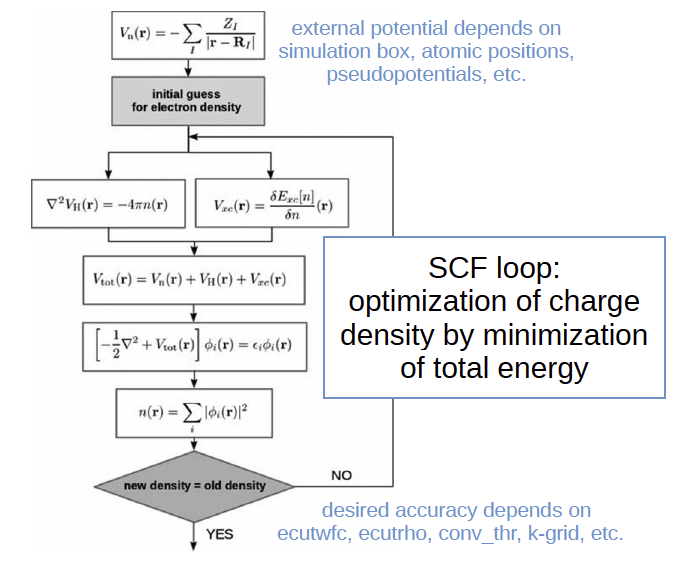
\includegraphics[width=0.85\textwidth]{figures/SCF.png}
\caption{Self-consistent field (SCF) loop schematic illustrating self-consistent electronic-structure workflow \cite{giustino2014materials}.}
\label{fig:SCF-loop}
\end{figure}


\begin{figure}[h!]
    \centering
    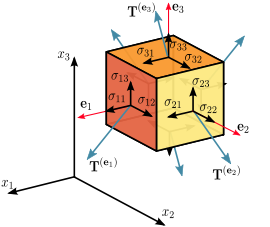
\includegraphics[width=0.6\textwidth]{Parts/Figures/Cij.png}
    \caption{Stress tensor visualization \cite{al2020non}.}
    \label{fig:seis-refl-tech}
\end{figure}

\begin{figure}[!ht]
	\centering
	\begin{subfigure}{0.9\textwidth}
         \centering
         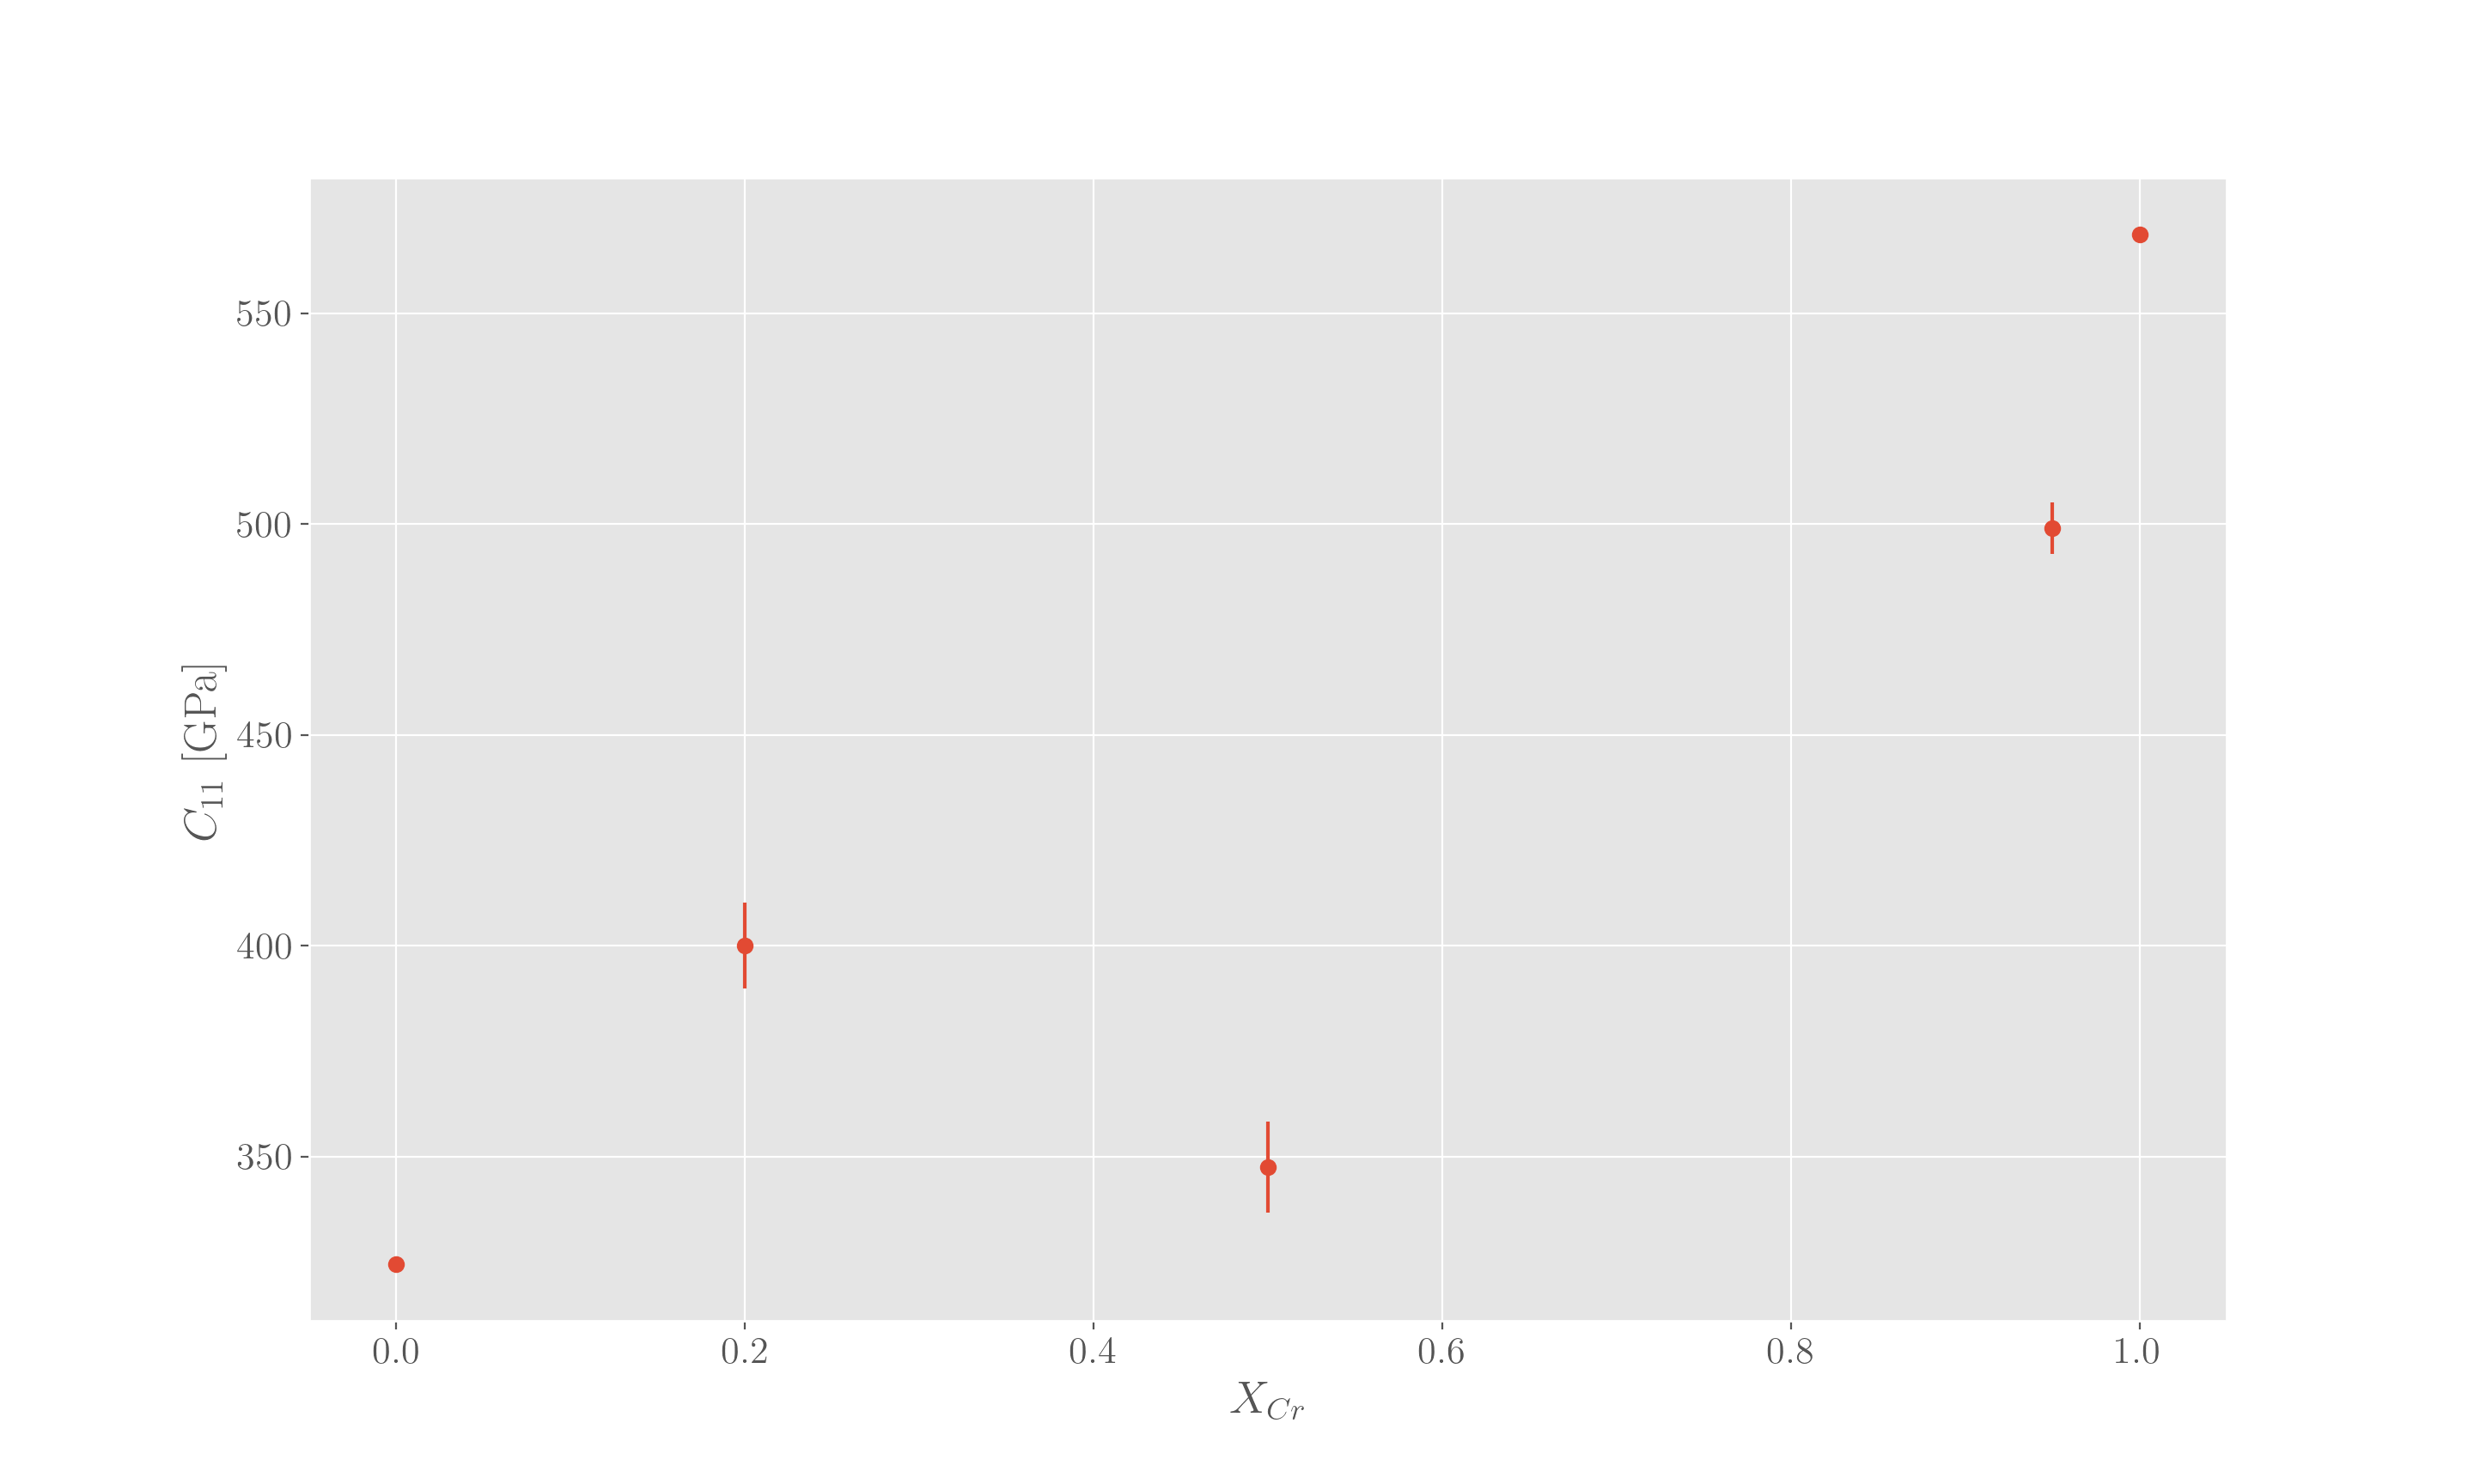
\includegraphics[width=\linewidth]{Parts/Figures/C11.png}
         \caption{Normal constant, \(C_{11}\), illustrating the longitudinal stiffness of bcc binary FeCr alloy as a function of chromium composition. This stiffness parameter is crucial for understanding the acoustic velocity and mechanical properties of the material.}
         \label{fig1a}
     \end{subfigure}
     \hfill
     \begin{subfigure}{0.45\textwidth}
         \centering
         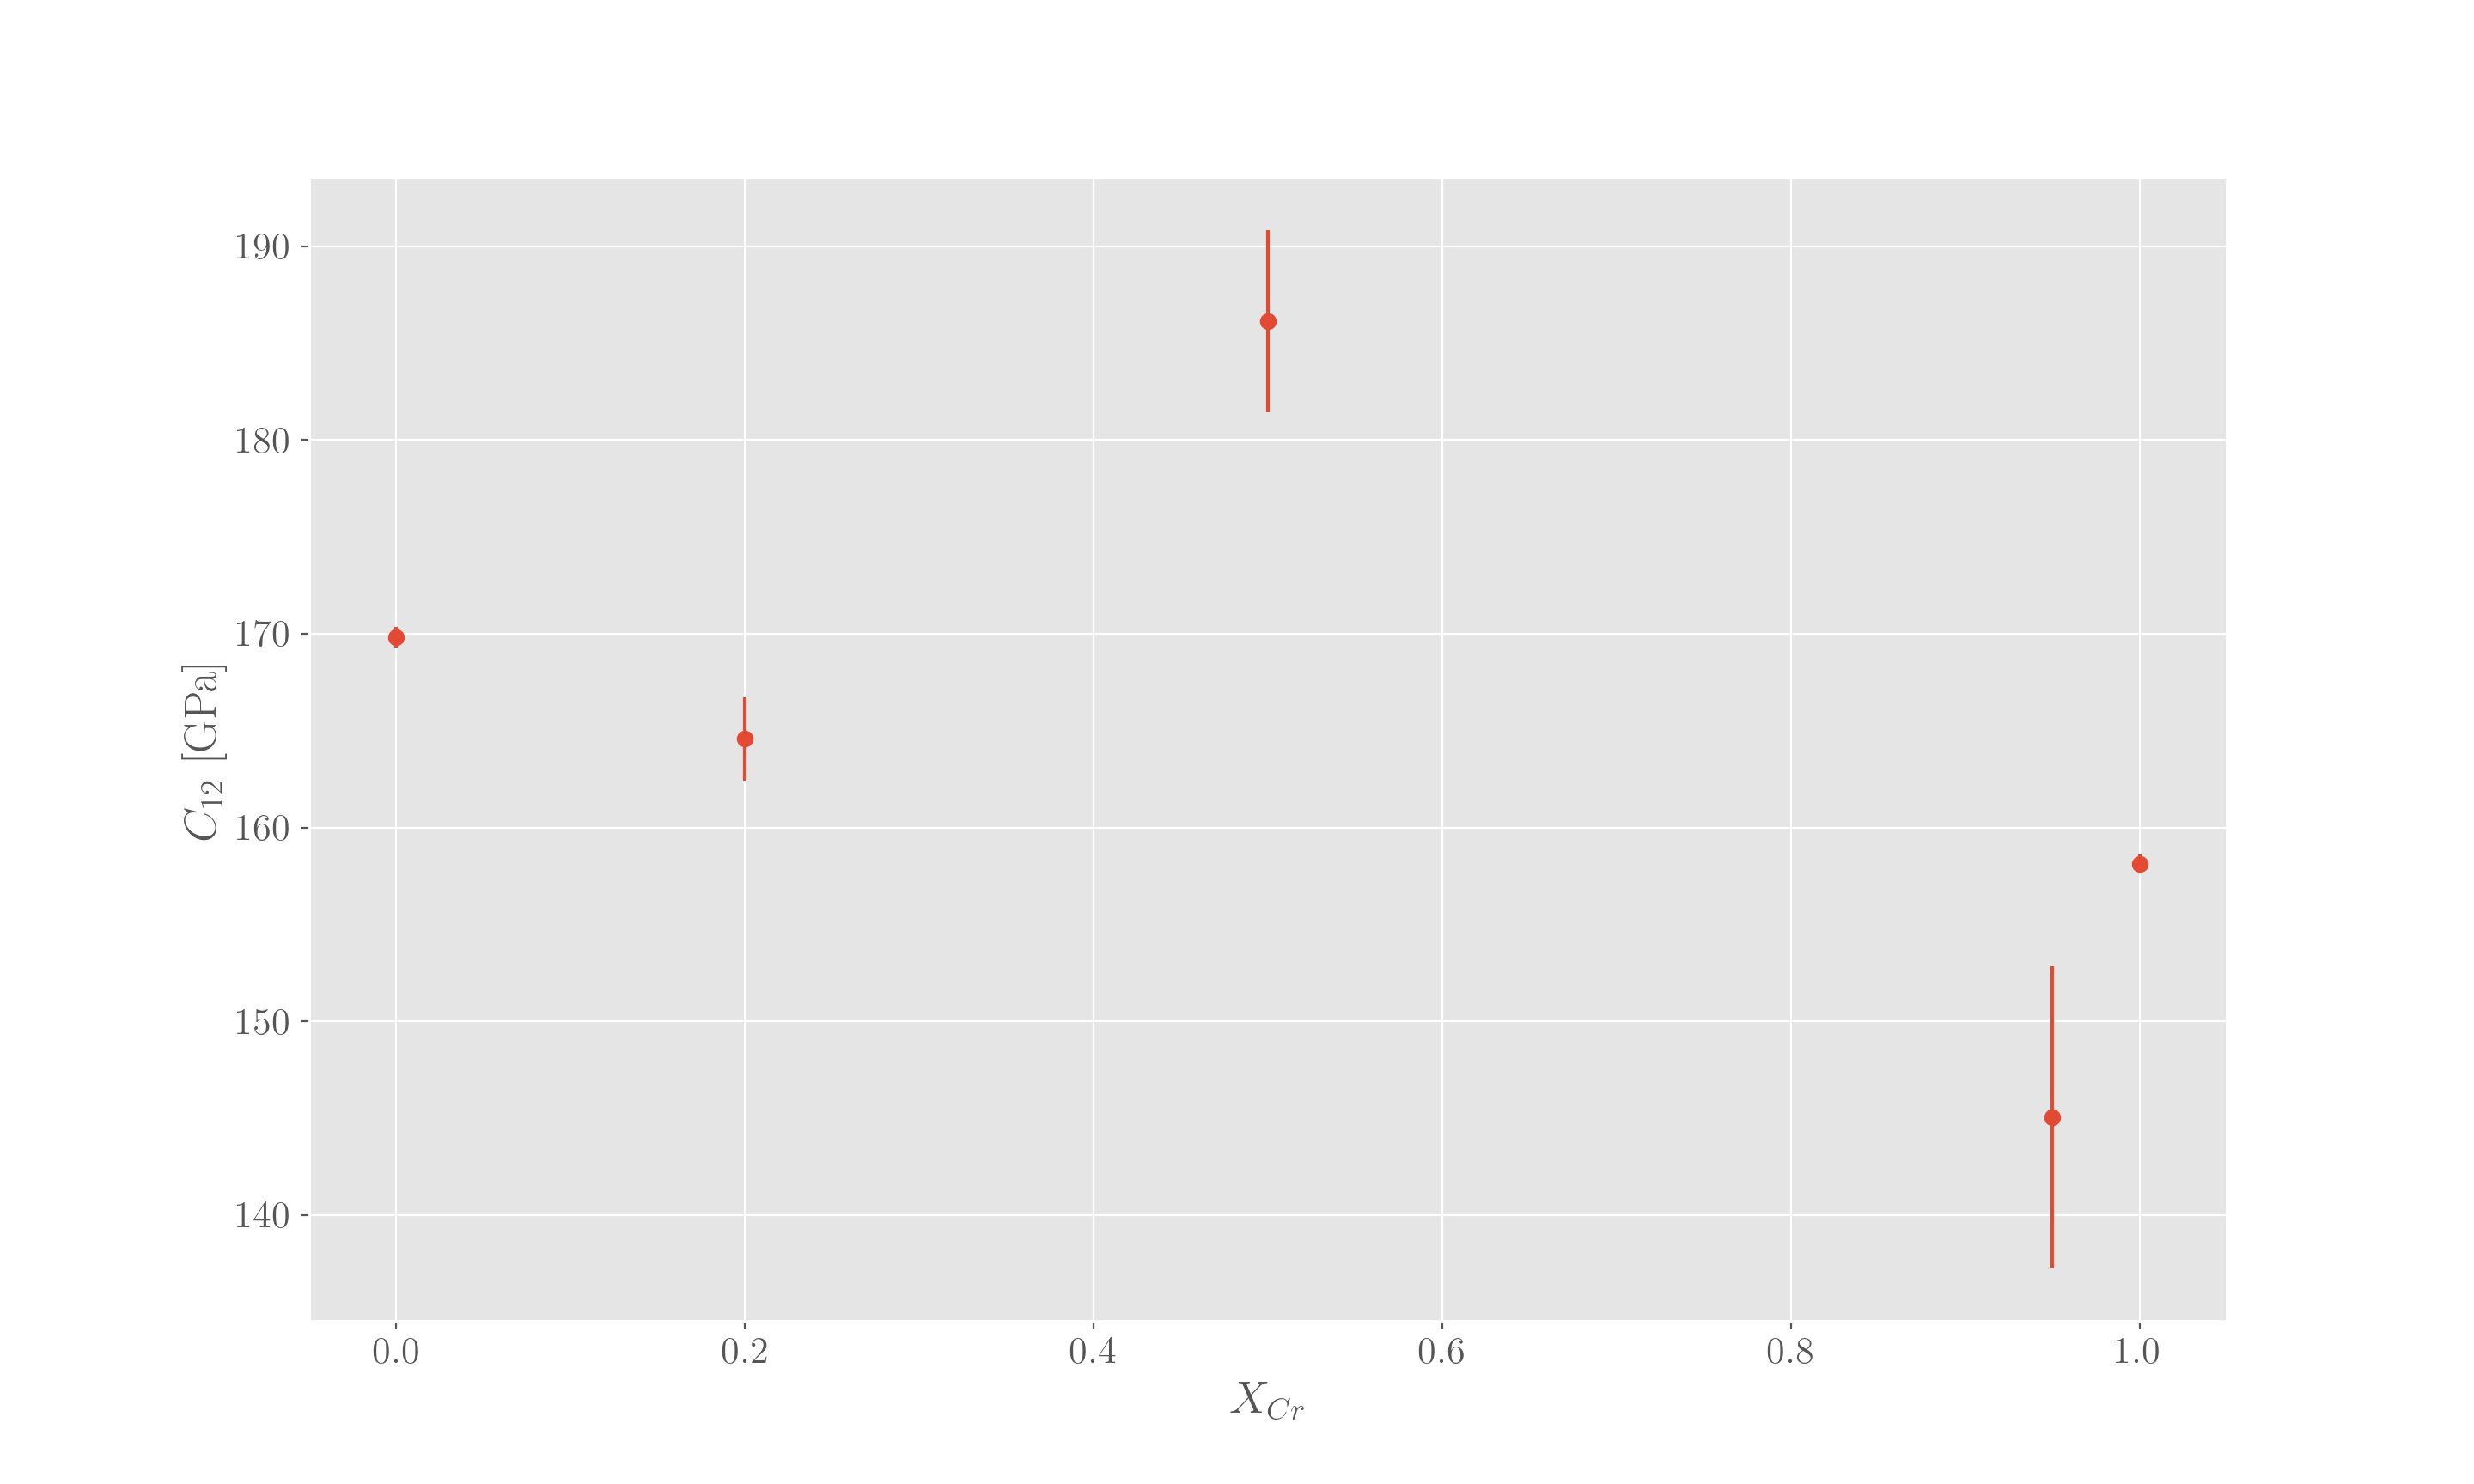
\includegraphics[width=\linewidth]{Parts/Figures/C12.png}
         \caption{The interplanar elastic constant \(C_{12}\), showing the coupling between axial and lateral strains, indicative of the alloy's resistance to shear along crystallographic planes.}
         \label{fig1b}
     \end{subfigure}
     \hfill
     \begin{subfigure}{0.45\textwidth}
         \centering
         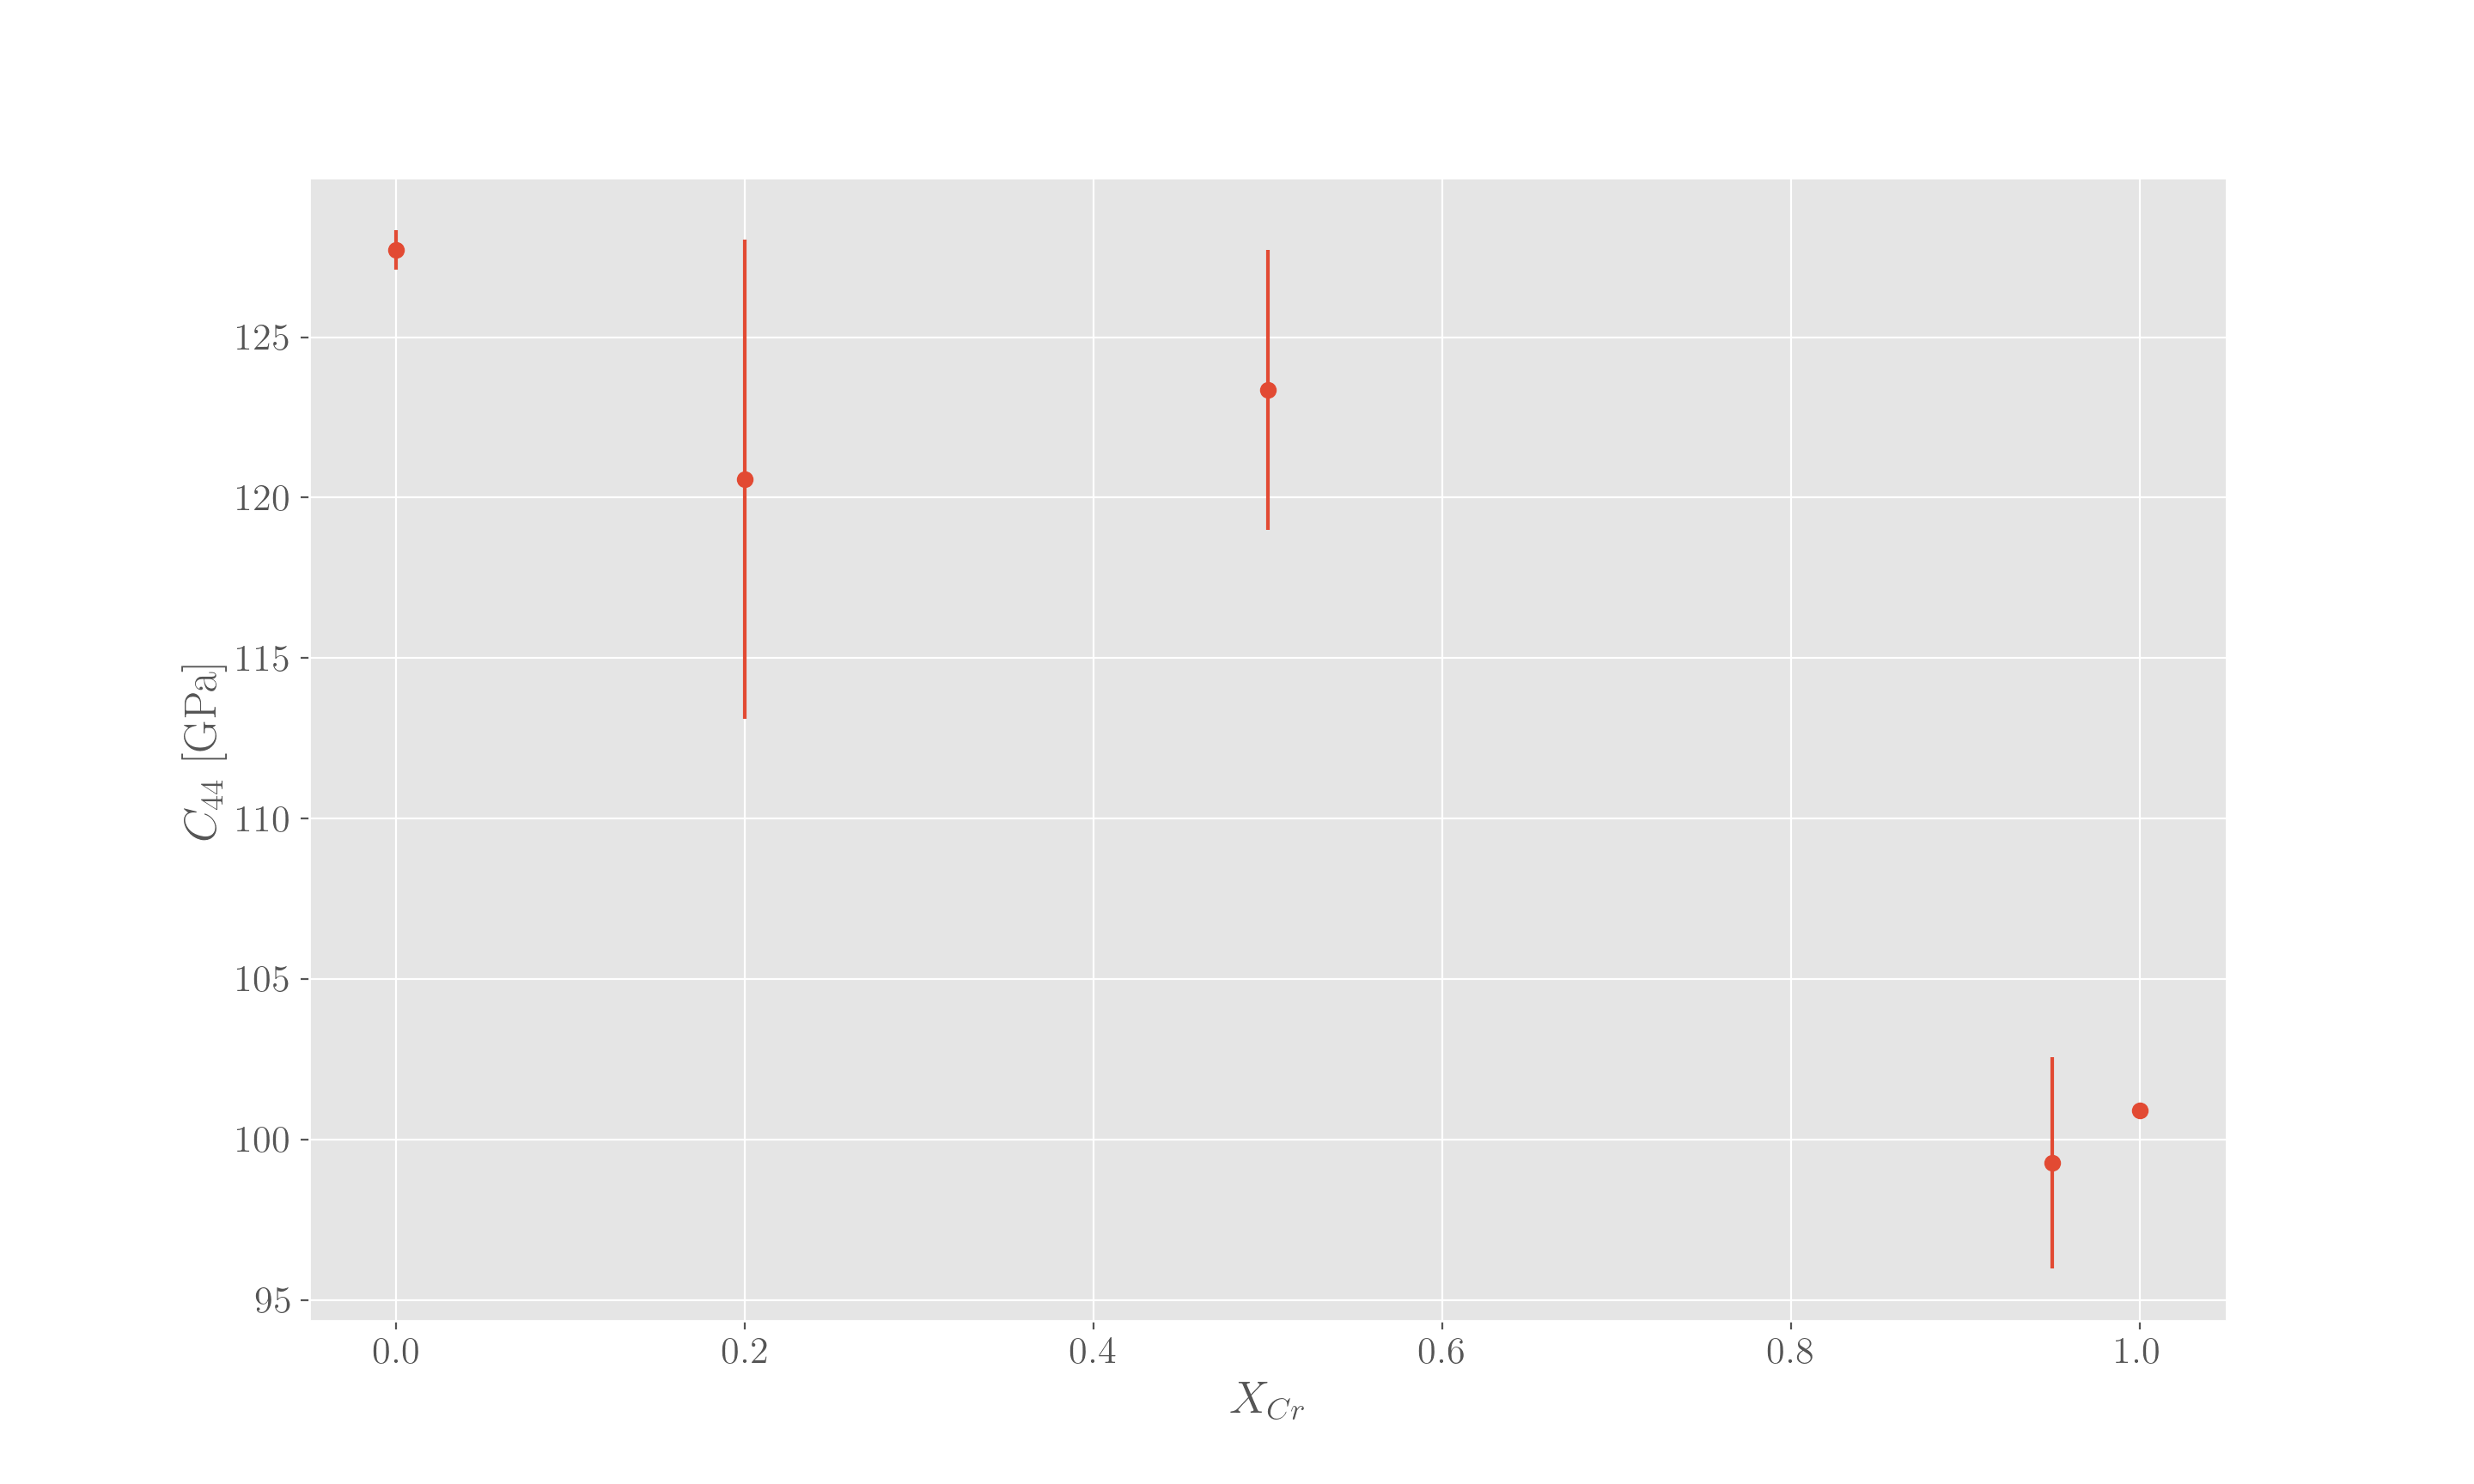
\includegraphics[width=\linewidth]{Parts/Figures/C44.png}
         \caption{Shear constant, \(C_{44}\), representing shear stiffness against deformation without volume change, critical for assessing material's resistance to applied shear stress.}
         \label{fig1c}
     \end{subfigure}
	\caption{Elastic constants of homogeneous bcc FeCr from the present DFT calculations (40-atom SQS) as a function of Cr composition. (a) Shows the longitudinal stiffness parameter \(C_{11}\), important for evaluating the material's response to compressive and tensile stresses. (b) Highlights \(C_{12}\), which is essential for understanding the coupling between different types of strain. (c) Details \(C_{44}\), crucial for evaluating the shear deformation behavior.}
	\label{fig1}
\end{figure}


\begin{figure}[!ht]
	\centering
	\begin{subfigure}{0.9\textwidth}
         \centering
         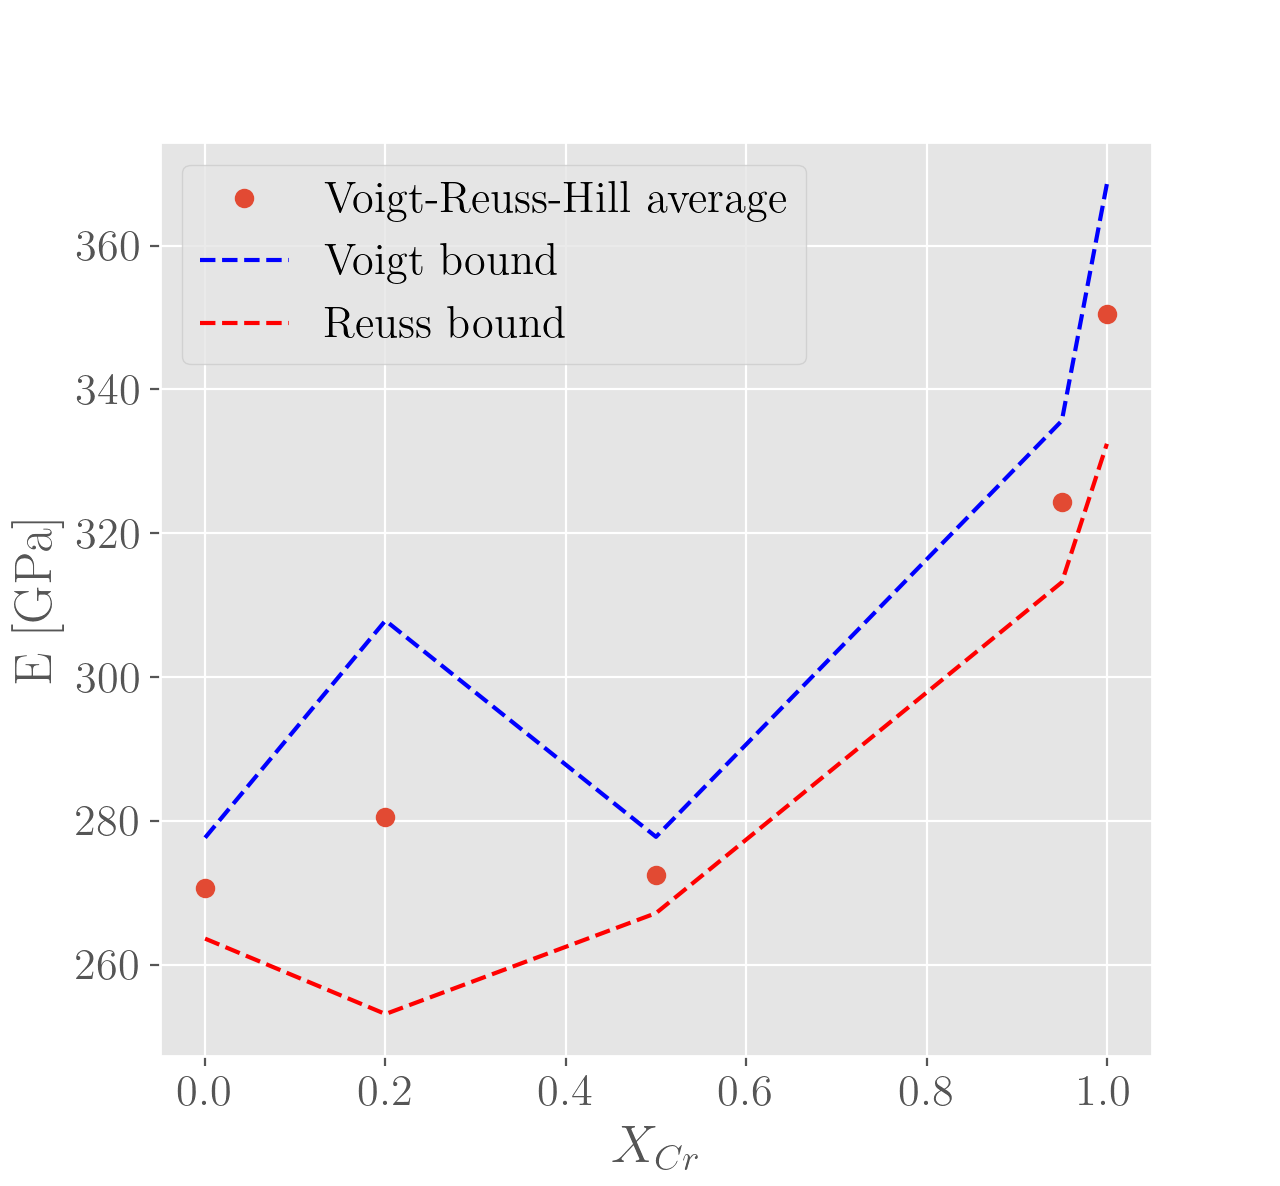
\includegraphics[width=0.9\linewidth]{Parts/Figures/E_VRH.png}
         \caption{Elastic (Young's) Modulus, \(E_{VRH}\), indicating the material's stiffness and its ability to resist deformation under tensile stress.}
         \label{fig2a}
     \end{subfigure}
     \hfill
     \begin{subfigure}{0.45\textwidth}
         \centering
         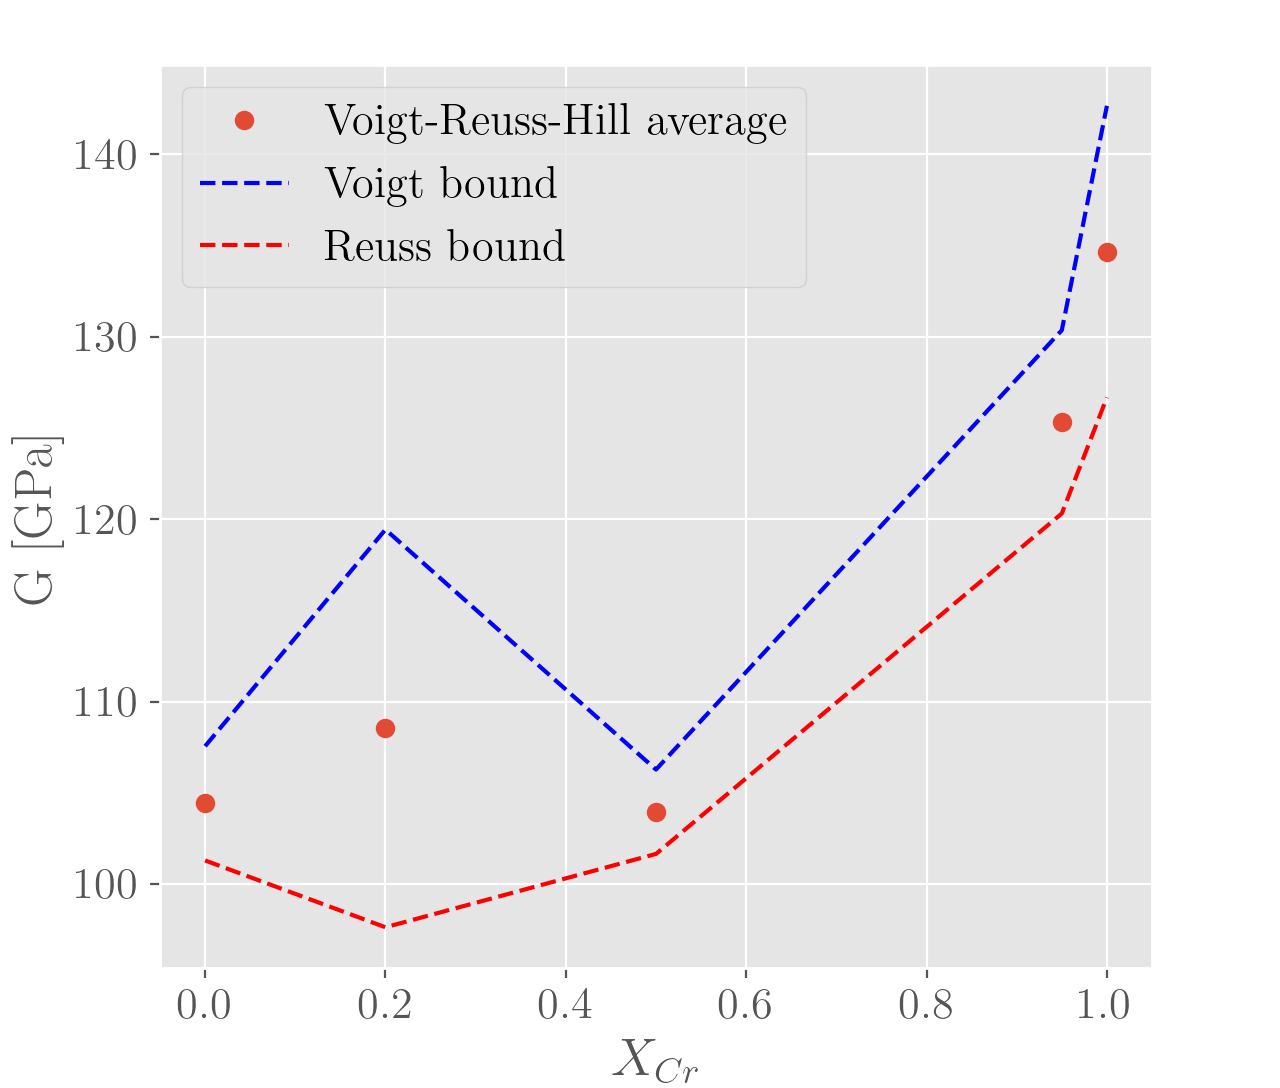
\includegraphics[width=\linewidth]{Parts/Figures/G_VRH.png}
         \caption{Shear modulus, \(G_{VRH}\), reflecting the material's ability to withstand shear deformation.}
         \label{fig2b}
     \end{subfigure}
     \hfill
     \begin{subfigure}{0.45\textwidth}
         \centering
         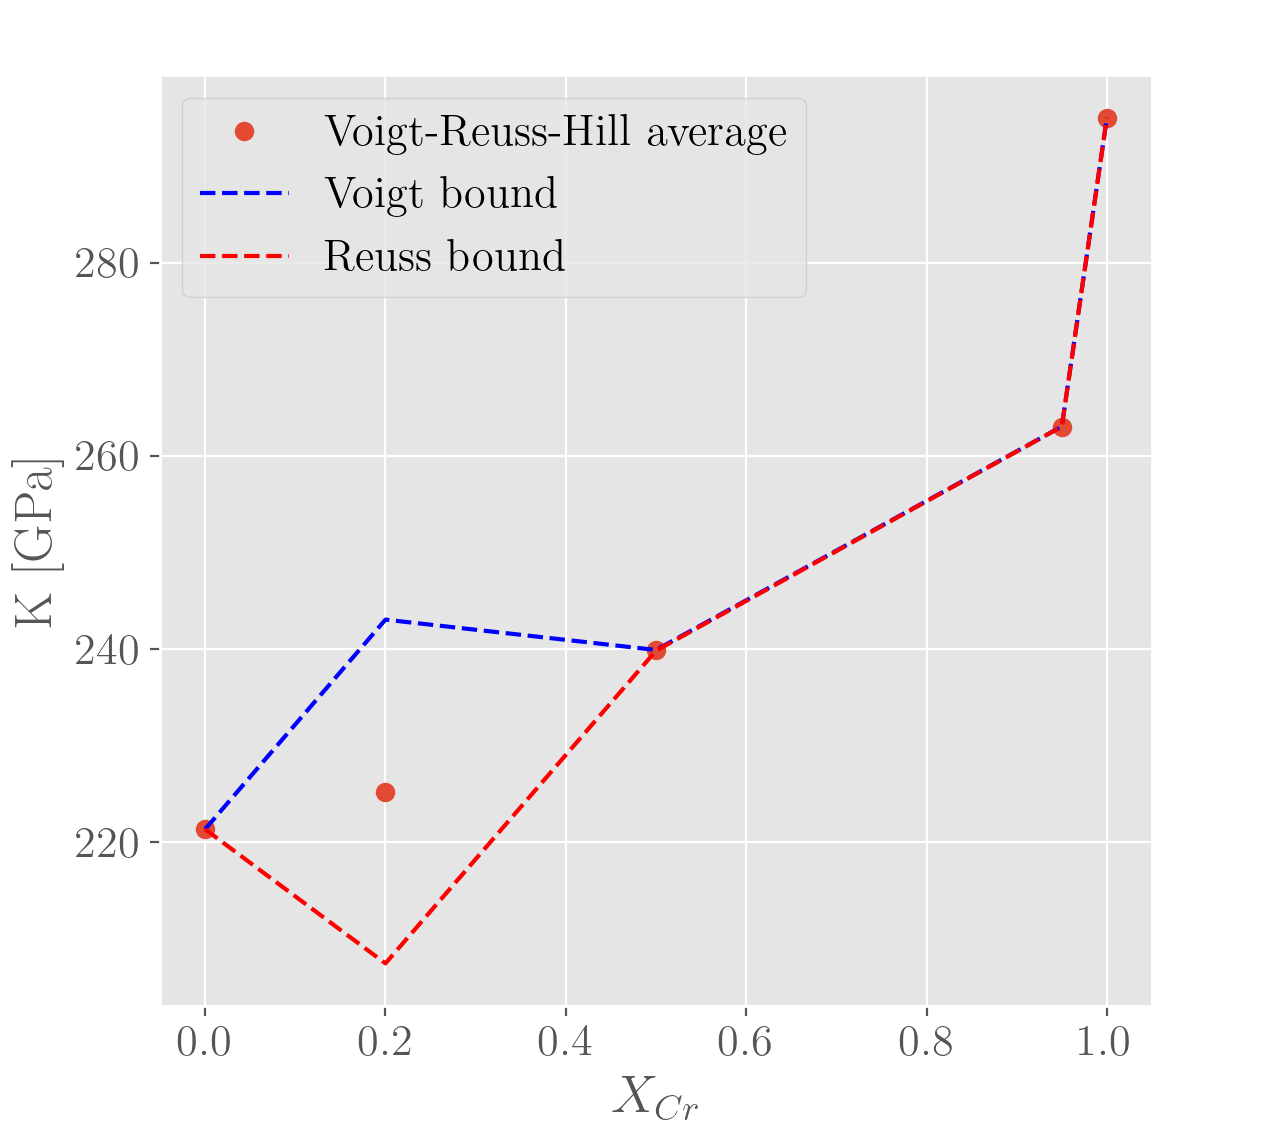
\includegraphics[width=\linewidth]{Parts/Figures/K_VRH.png}
         \caption{Bulk modulus, \(K_{VRH}\), which measures the material's resistance to uniform compression.}
         \label{fig2c}
     \end{subfigure}
	\caption{VRH elastic moduli of homogeneous bcc FeCr from the present DFT calculations as a function of Cr composition. (a) Elastic (Young's) Modulus demonstrates the material's overall stiffness. (b) Shear modulus is a measure of the alloy's rigidity against shear forces. (c) Bulk modulus assesses the material's compressibility under uniform pressure.}
	\label{fig2}
\end{figure}

\begin{sidewaysfigure}[!ht]
	\centering
	\begin{subfigure}{0.7\textwidth}
         \centering
         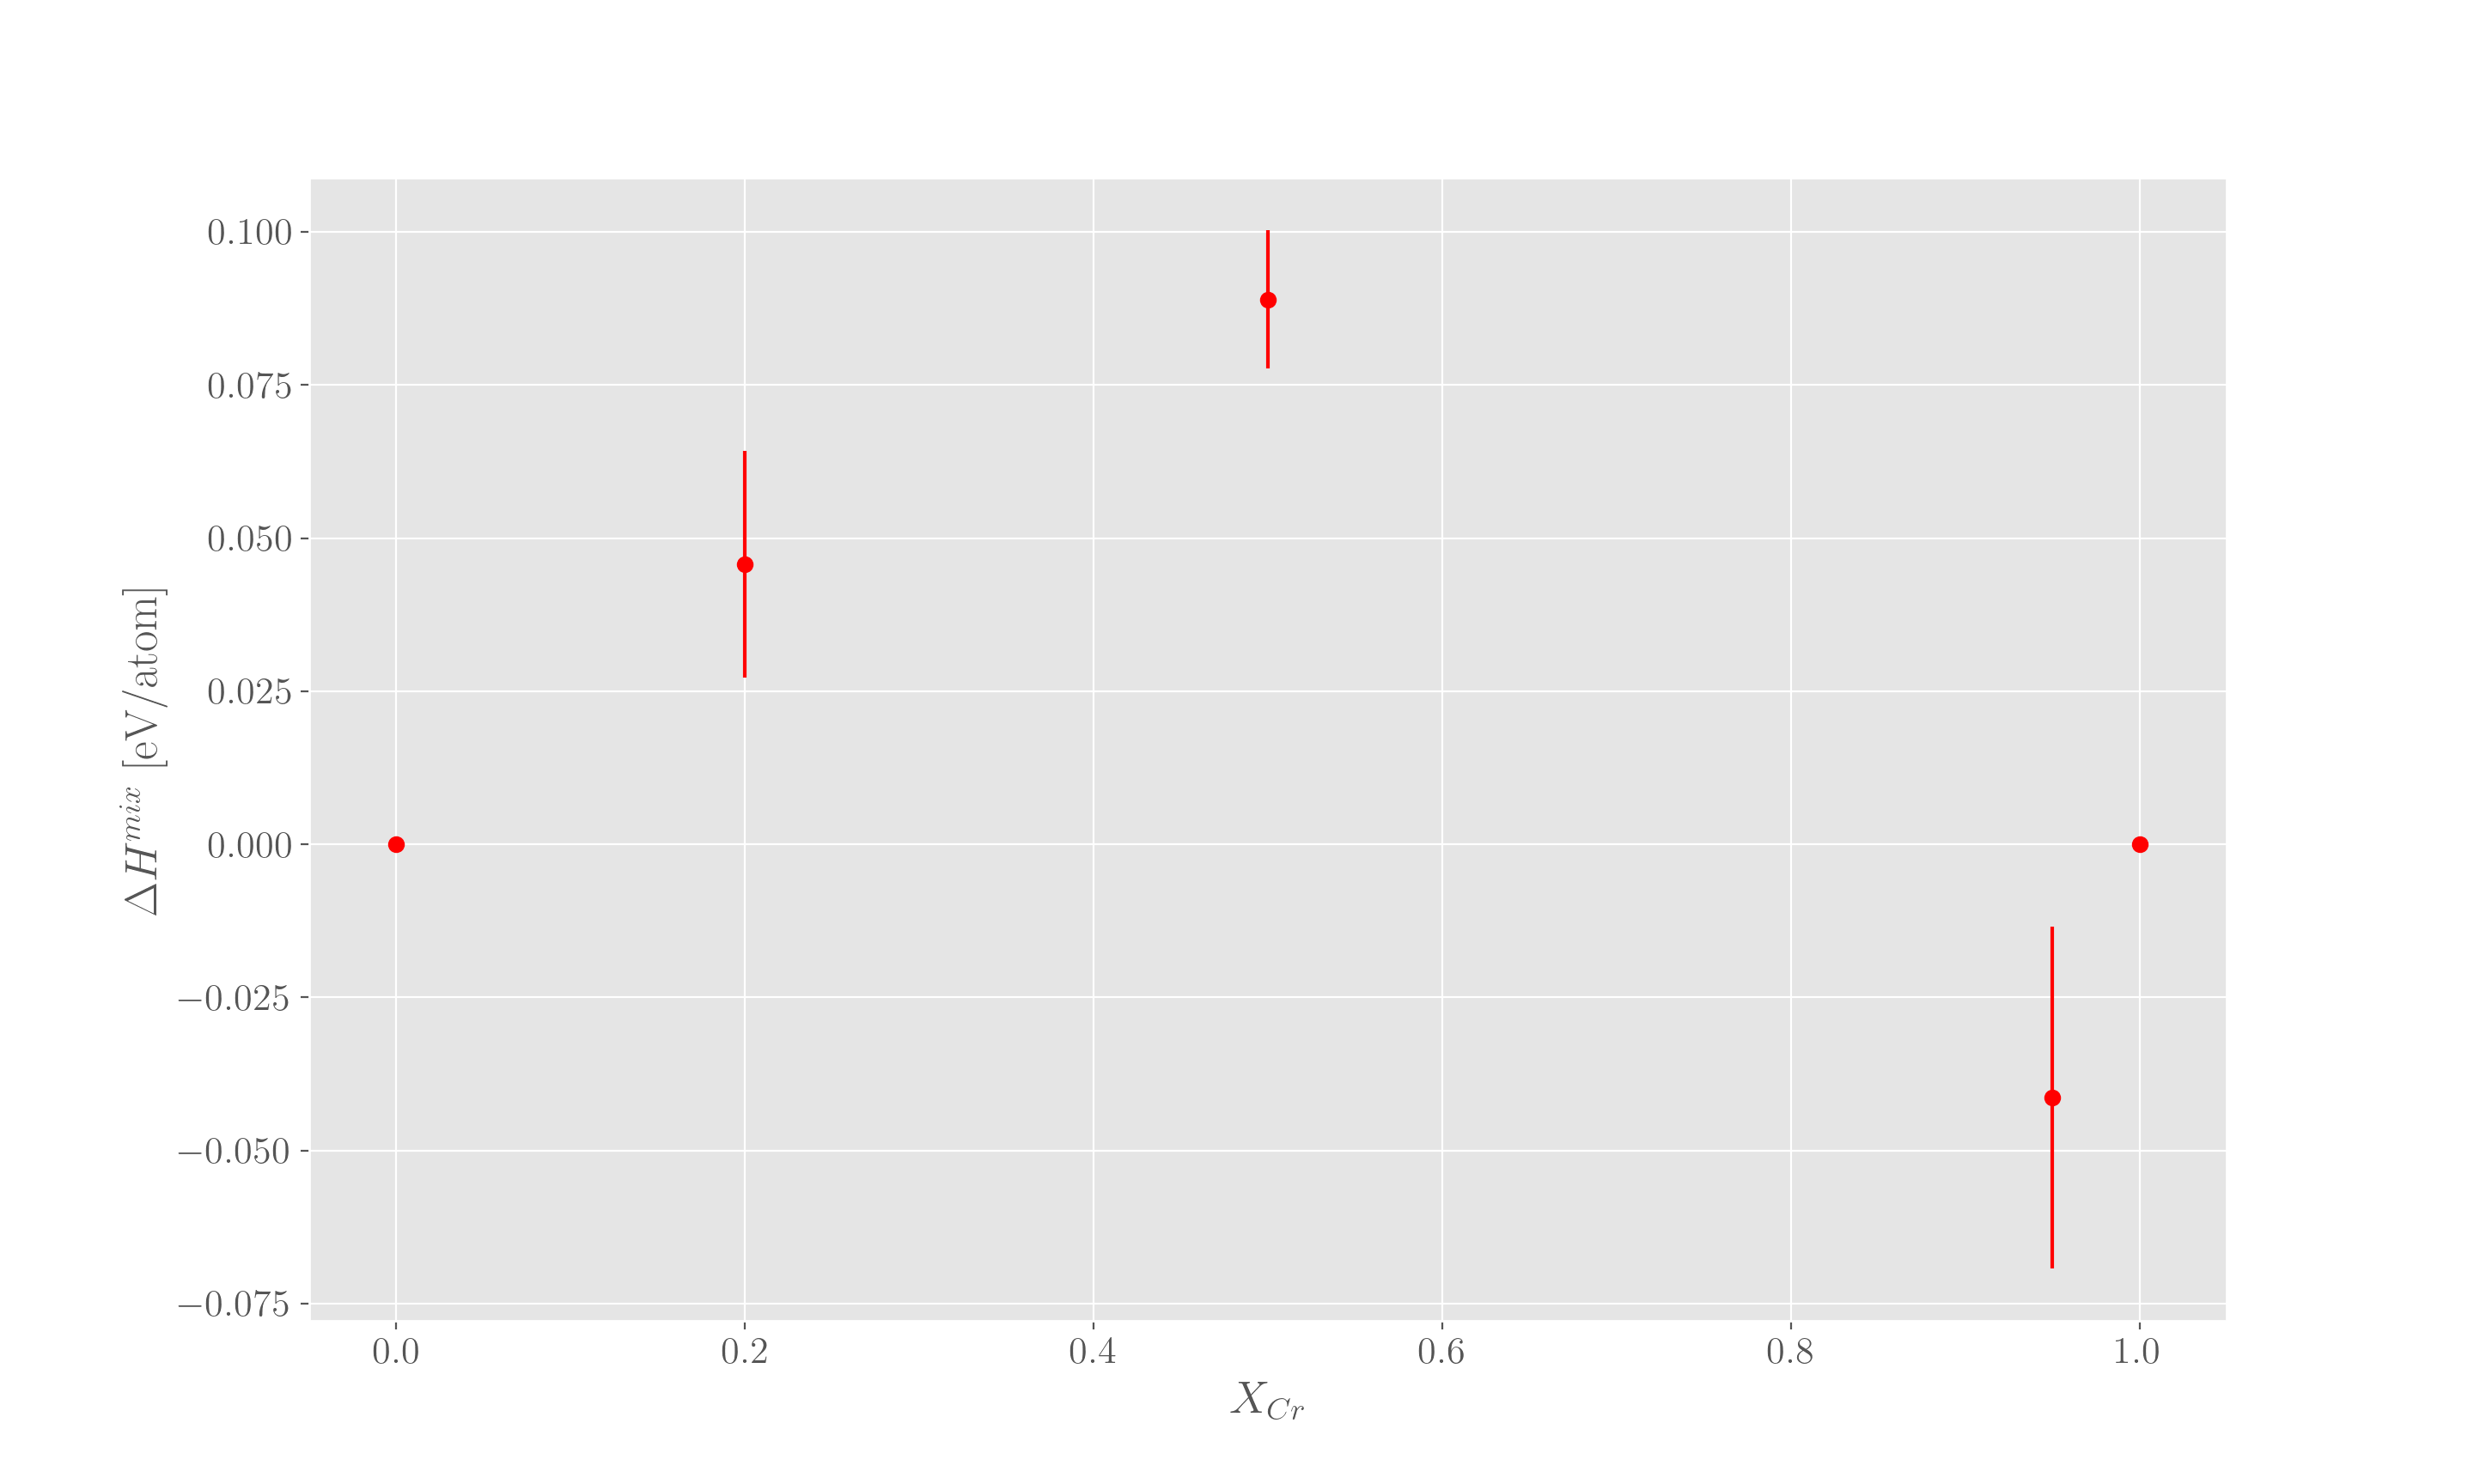
\includegraphics[width=\linewidth]{Parts/Figures/Hmix-vF.png}
         \caption{Enthalpy of mixing, showing the thermodynamic favorability of phase separation in bcc $\delta$-ferrite in cast austenitic stainless steels through spinodal decomposition.}
         \label{fig3a}
     \end{subfigure}
     \begin{subfigure}{0.3\textwidth}
         \centering
         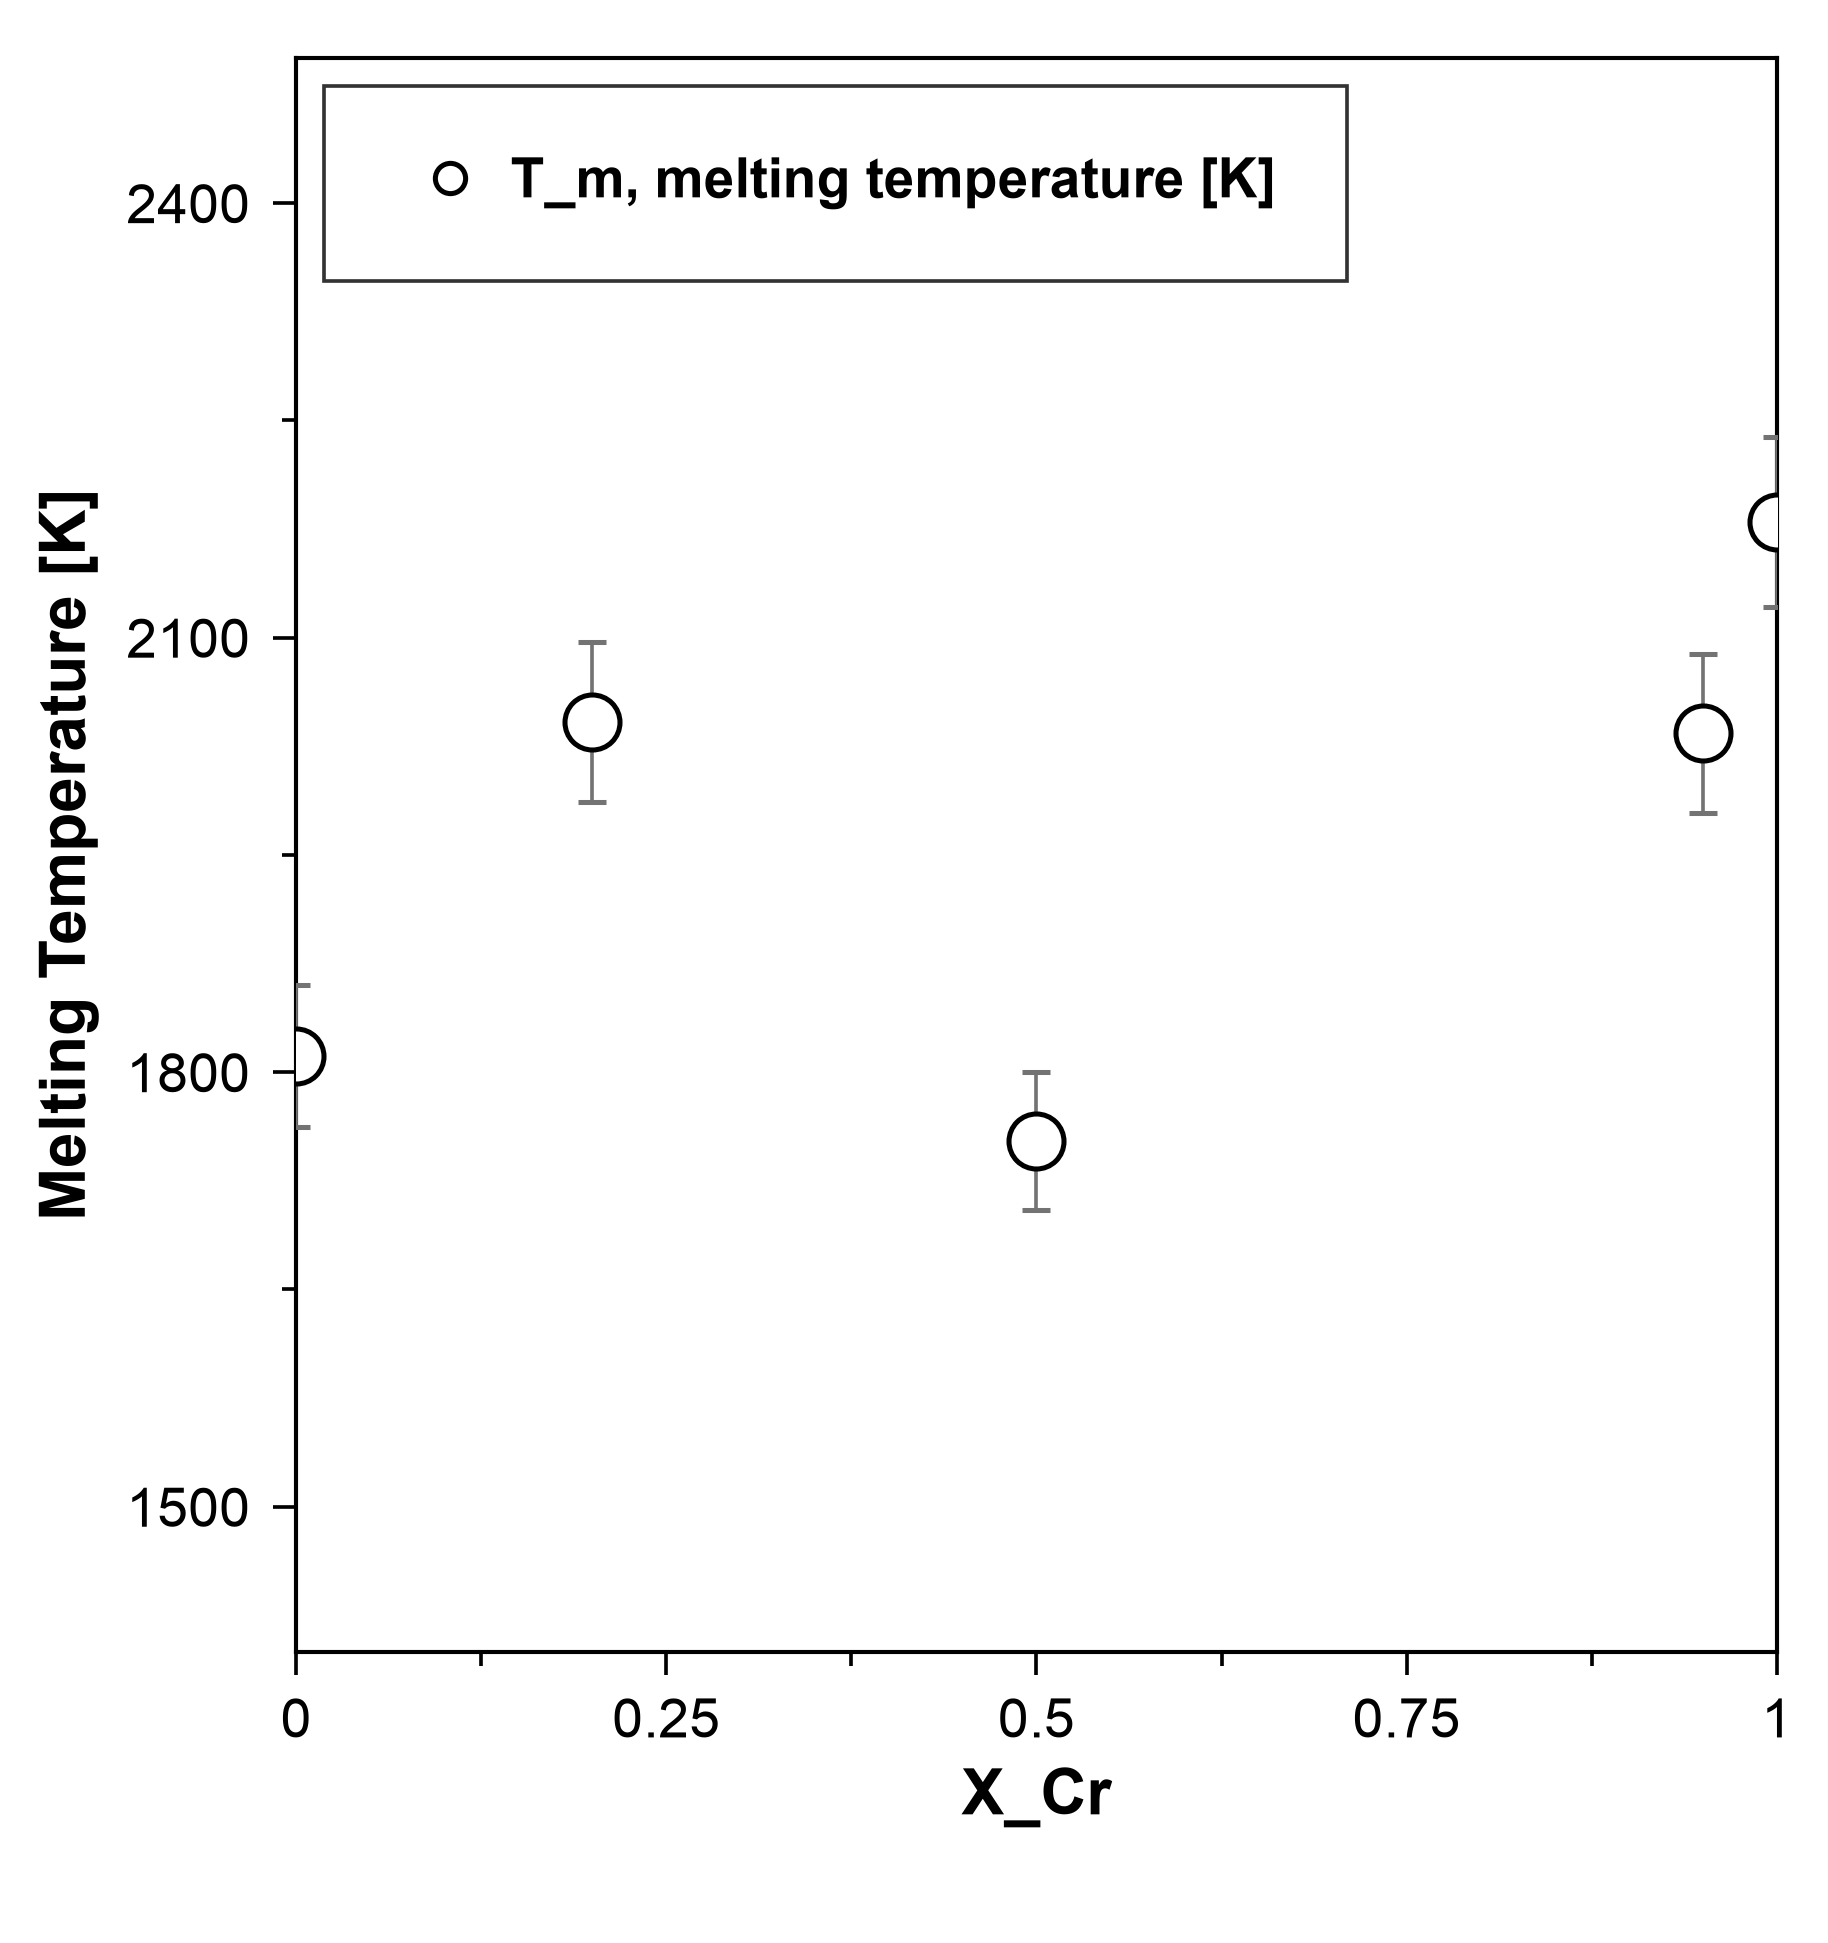
\includegraphics[width=\linewidth]{Parts/Figures/TMvsX_v3.png}
         \caption{\(T_M\), melting temperature, indicating how the thermal stability of the material changes with Cr composition.}
         \label{fig3b}
     \end{subfigure}
     \begin{subfigure}{0.3\textwidth}
         \centering
         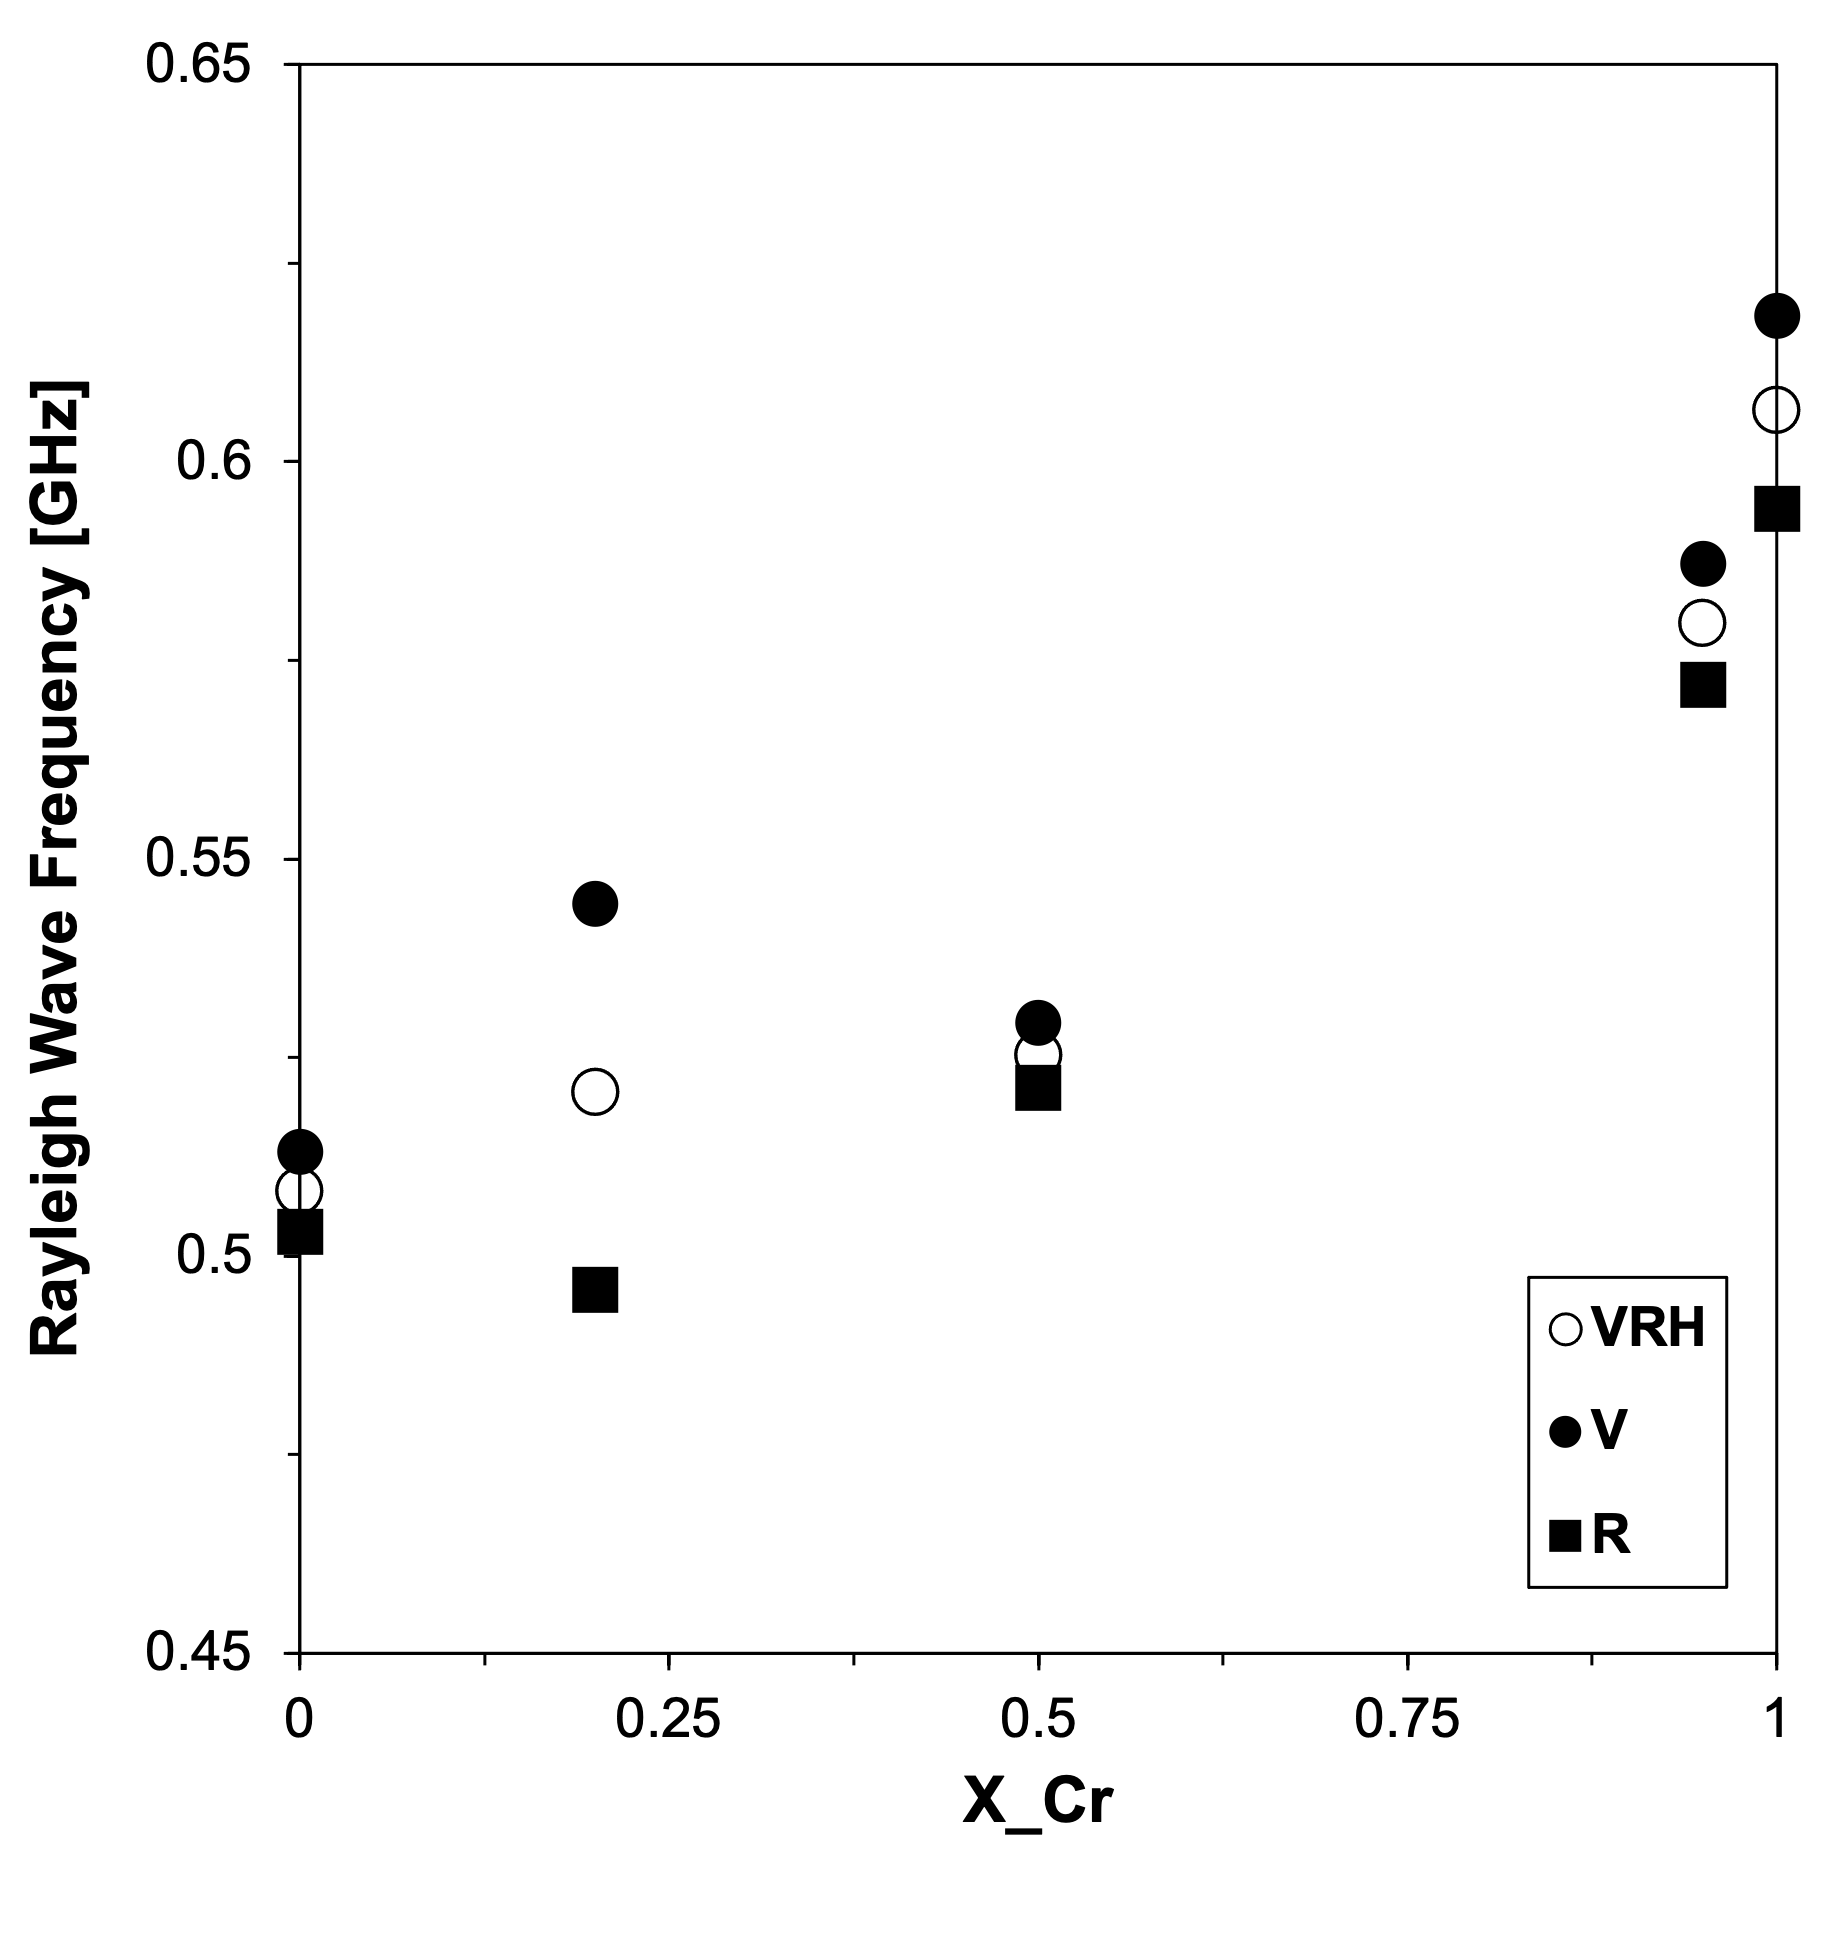
\includegraphics[width=\linewidth]{Parts/Figures/f_rwVsX_vF.png}
         \caption{Rayleigh wave frequencies, illustrating the impact of spinodal decomposition on the material's surface acoustic properties.}
         \label{fig3c}
     \end{subfigure}
     \begin{subfigure}{0.3\textwidth}
         \centering
         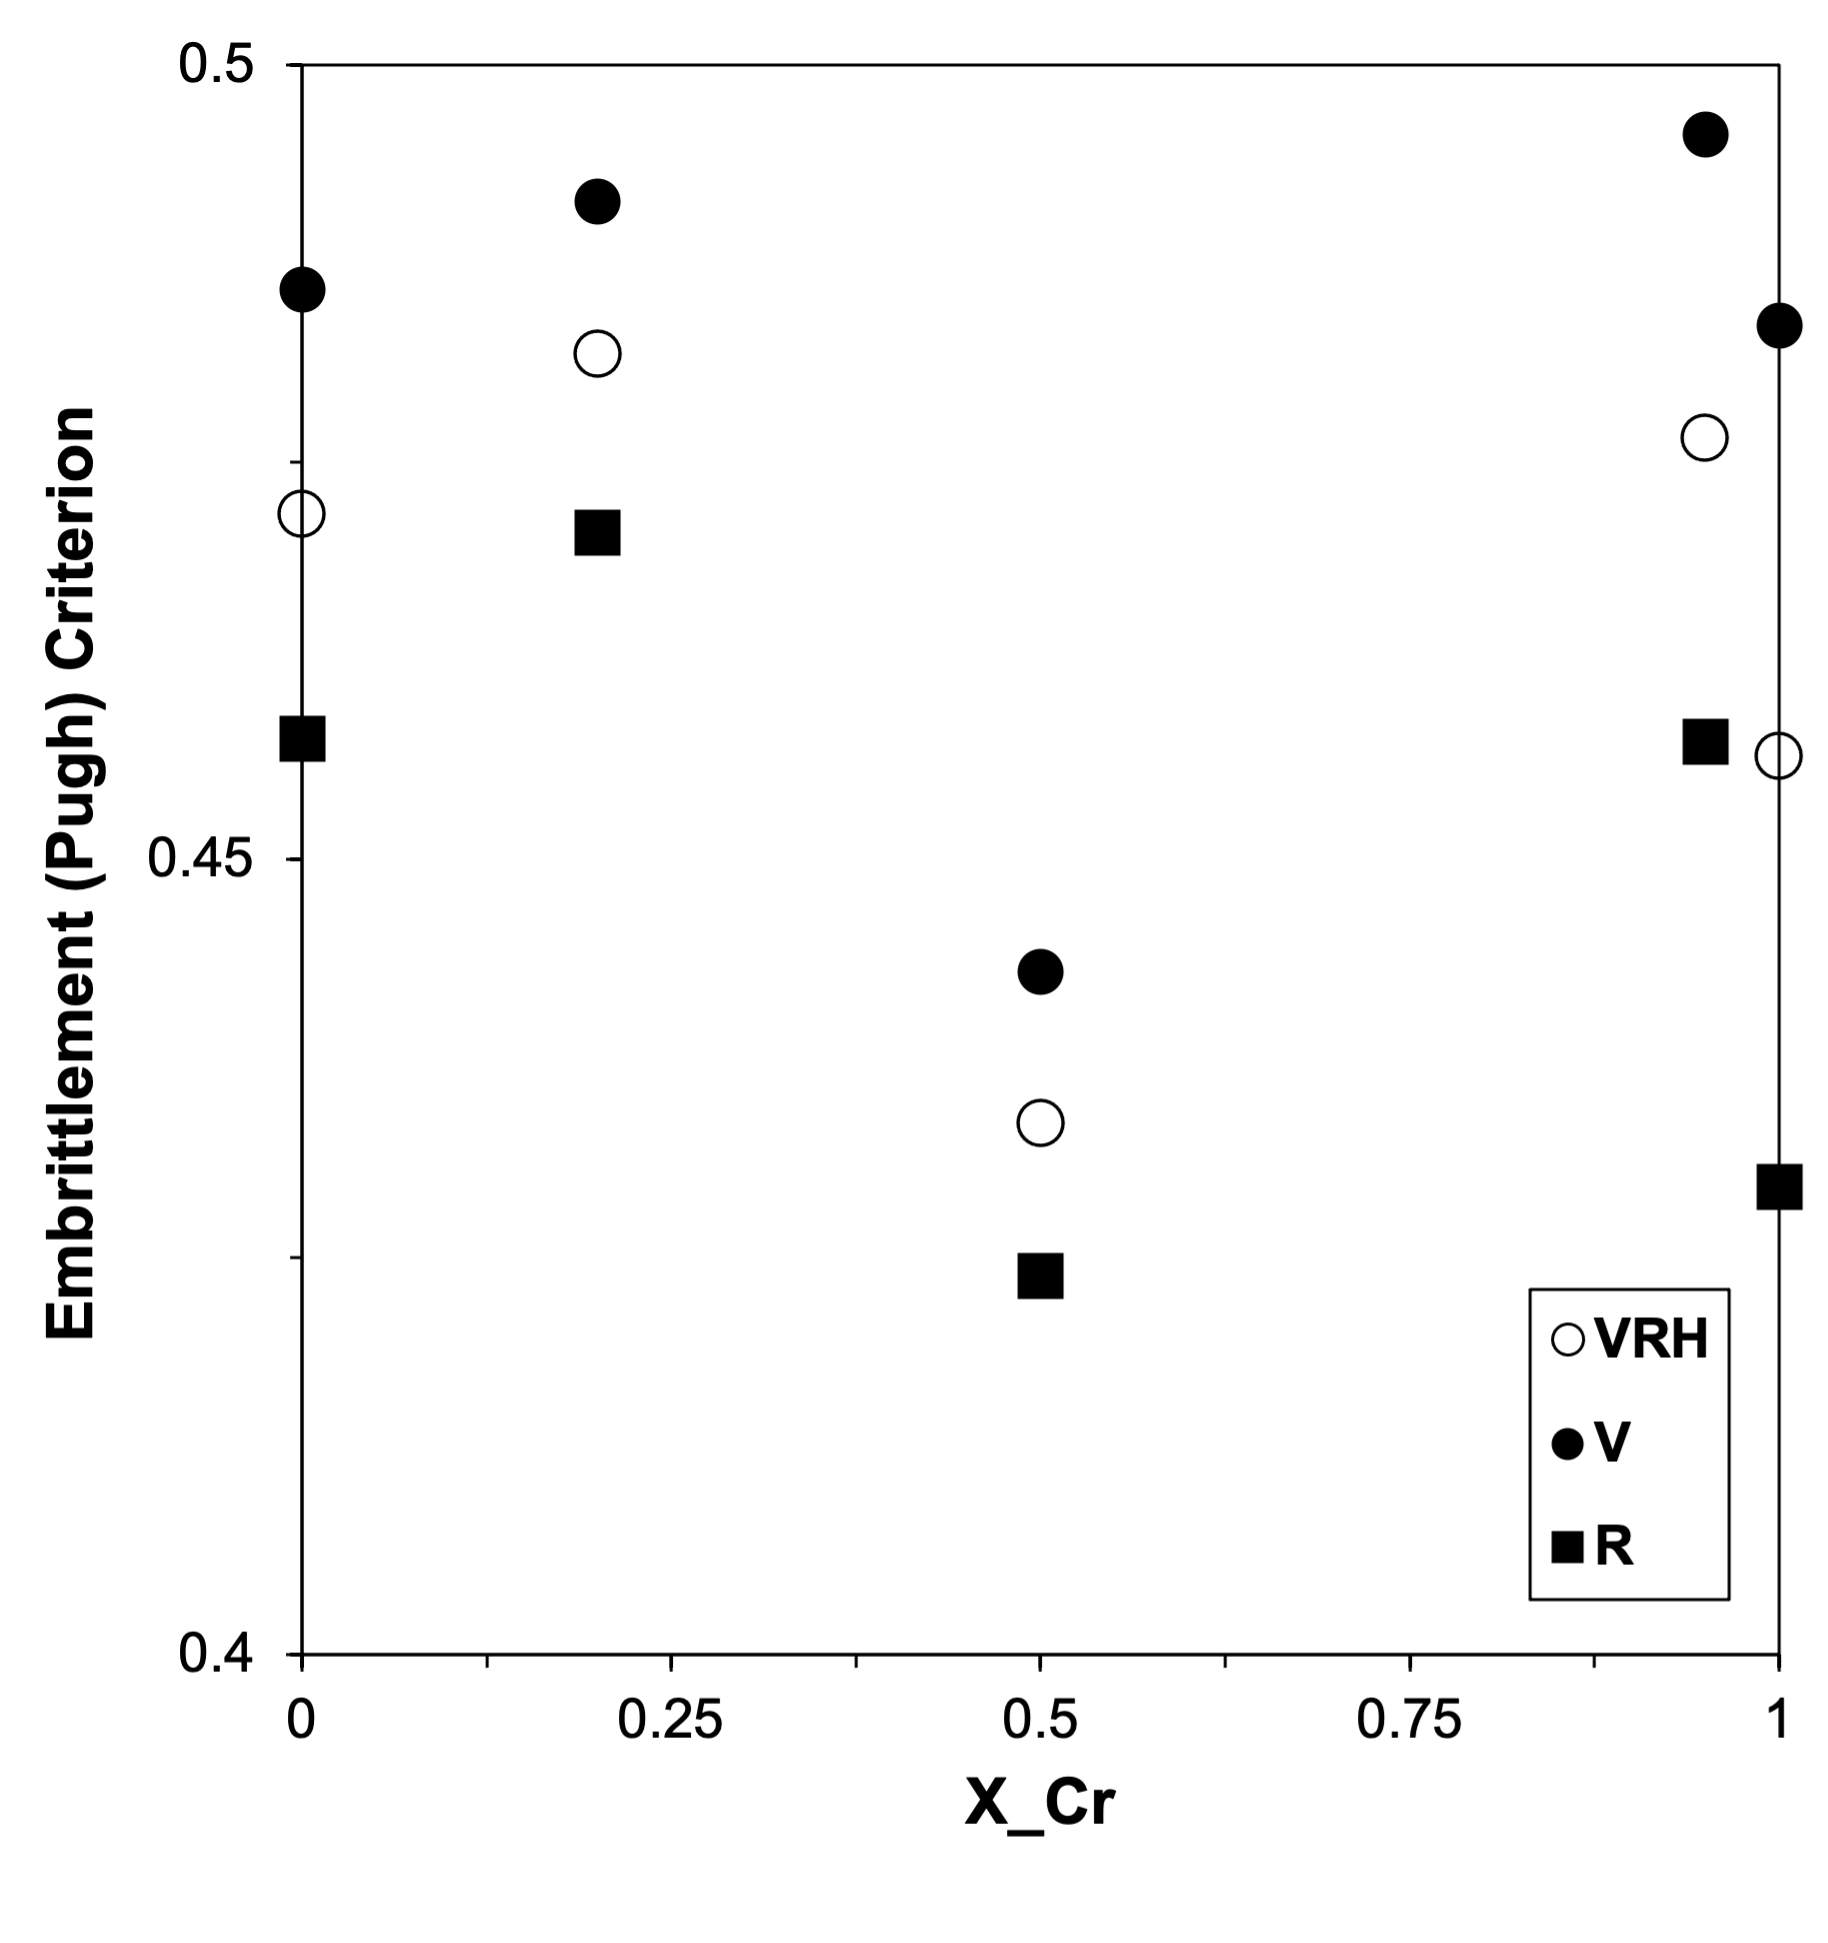
\includegraphics[width=\linewidth]{Parts/Figures/EvsX_vF.png}
         \caption{Embrittlement (Pugh) Criterion, calculated to evaluate the embrittlement risk associated with varying Cr compositions.}
         \label{fig3d}
     \end{subfigure}
	\caption{(a) The enthalpy of mixing demonstrates the thermodynamic drive towards phase separation indicative of spinodal decomposition, affecting the material's mechanical integrity. (b) Variations in the melting temperature as a function of Cr composition offer insights into the thermal stability and potential phase transformations within the alloy. The melting temperature is the Lindemann estimate $T_m=0.00321\,f^2 M V^{2/3}\Theta_D^2$ ($M$ in g/mol, $V$ in cm$^3$/mol) from the present VASP tensors, with $\Theta_D$ from the Debye average of the VRH sound speeds and the Lindemann constant $f$ calibrated on the measured melting points of Fe (1811~K) and Cr (2180~K); this corrects the original panel, which used Planck's constant in place of $k_B$ and the arithmetic mean of the sound speeds. (c) Changes in Rayleigh wave frequencies across compositions highlight alterations in surface acoustic properties, correlating with mechanical behavior. (d) The Embrittlement (Pugh) Criterion allows for assessing the risk of material embrittlement due to changes in composition, crucial for ensuring material reliability in critical applications.}
	\label{fig3}
\end{sidewaysfigure}


\begin{sidewaysfigure}[!ht]
    \centering
    \begin{subfigure}{0.9\textwidth}
        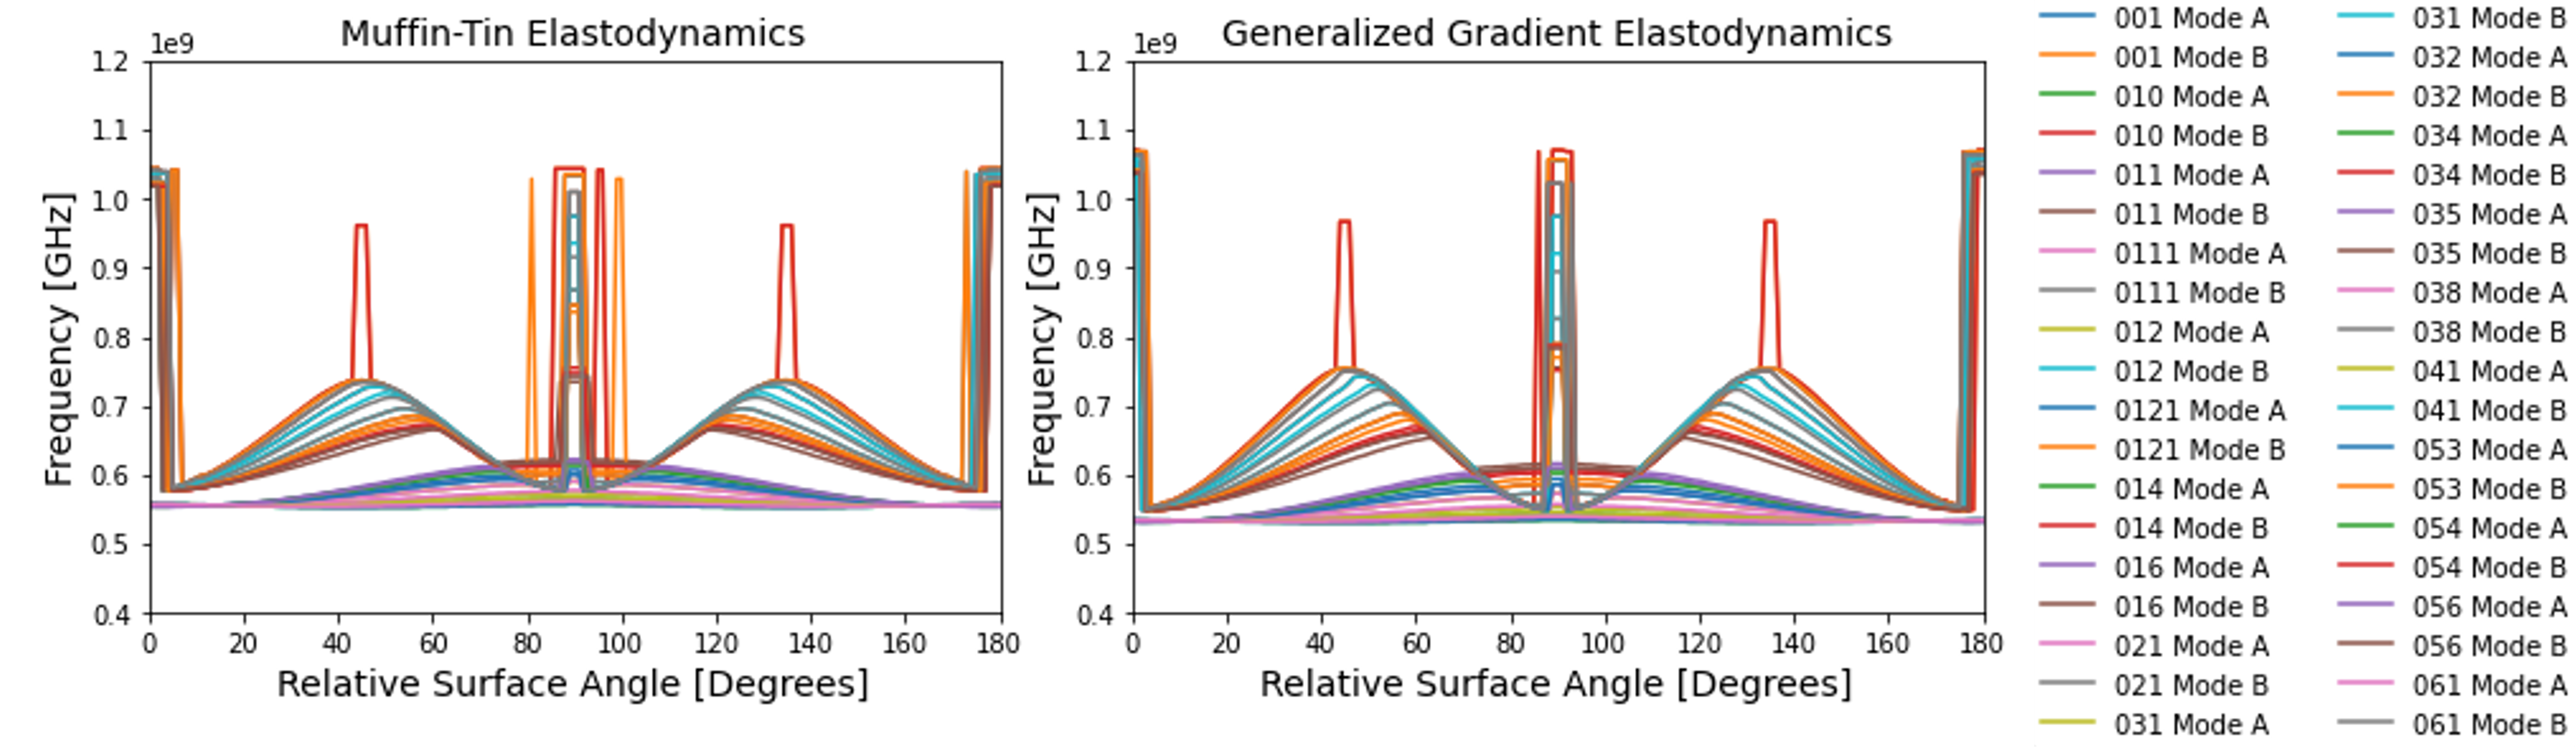
\includegraphics[width=\textwidth]{Parts/Figures/smoking-gun-v2.png}
        \caption{Predicted elastic frequencies showcasing the emergence of new modes within the elastodynamically-unallowed regions, signifying alterations in the material's mechanical properties due to spinodal decomposition.}
        \label{fig4a}
    \end{subfigure}
    \begin{subfigure}{0.35\textwidth}
        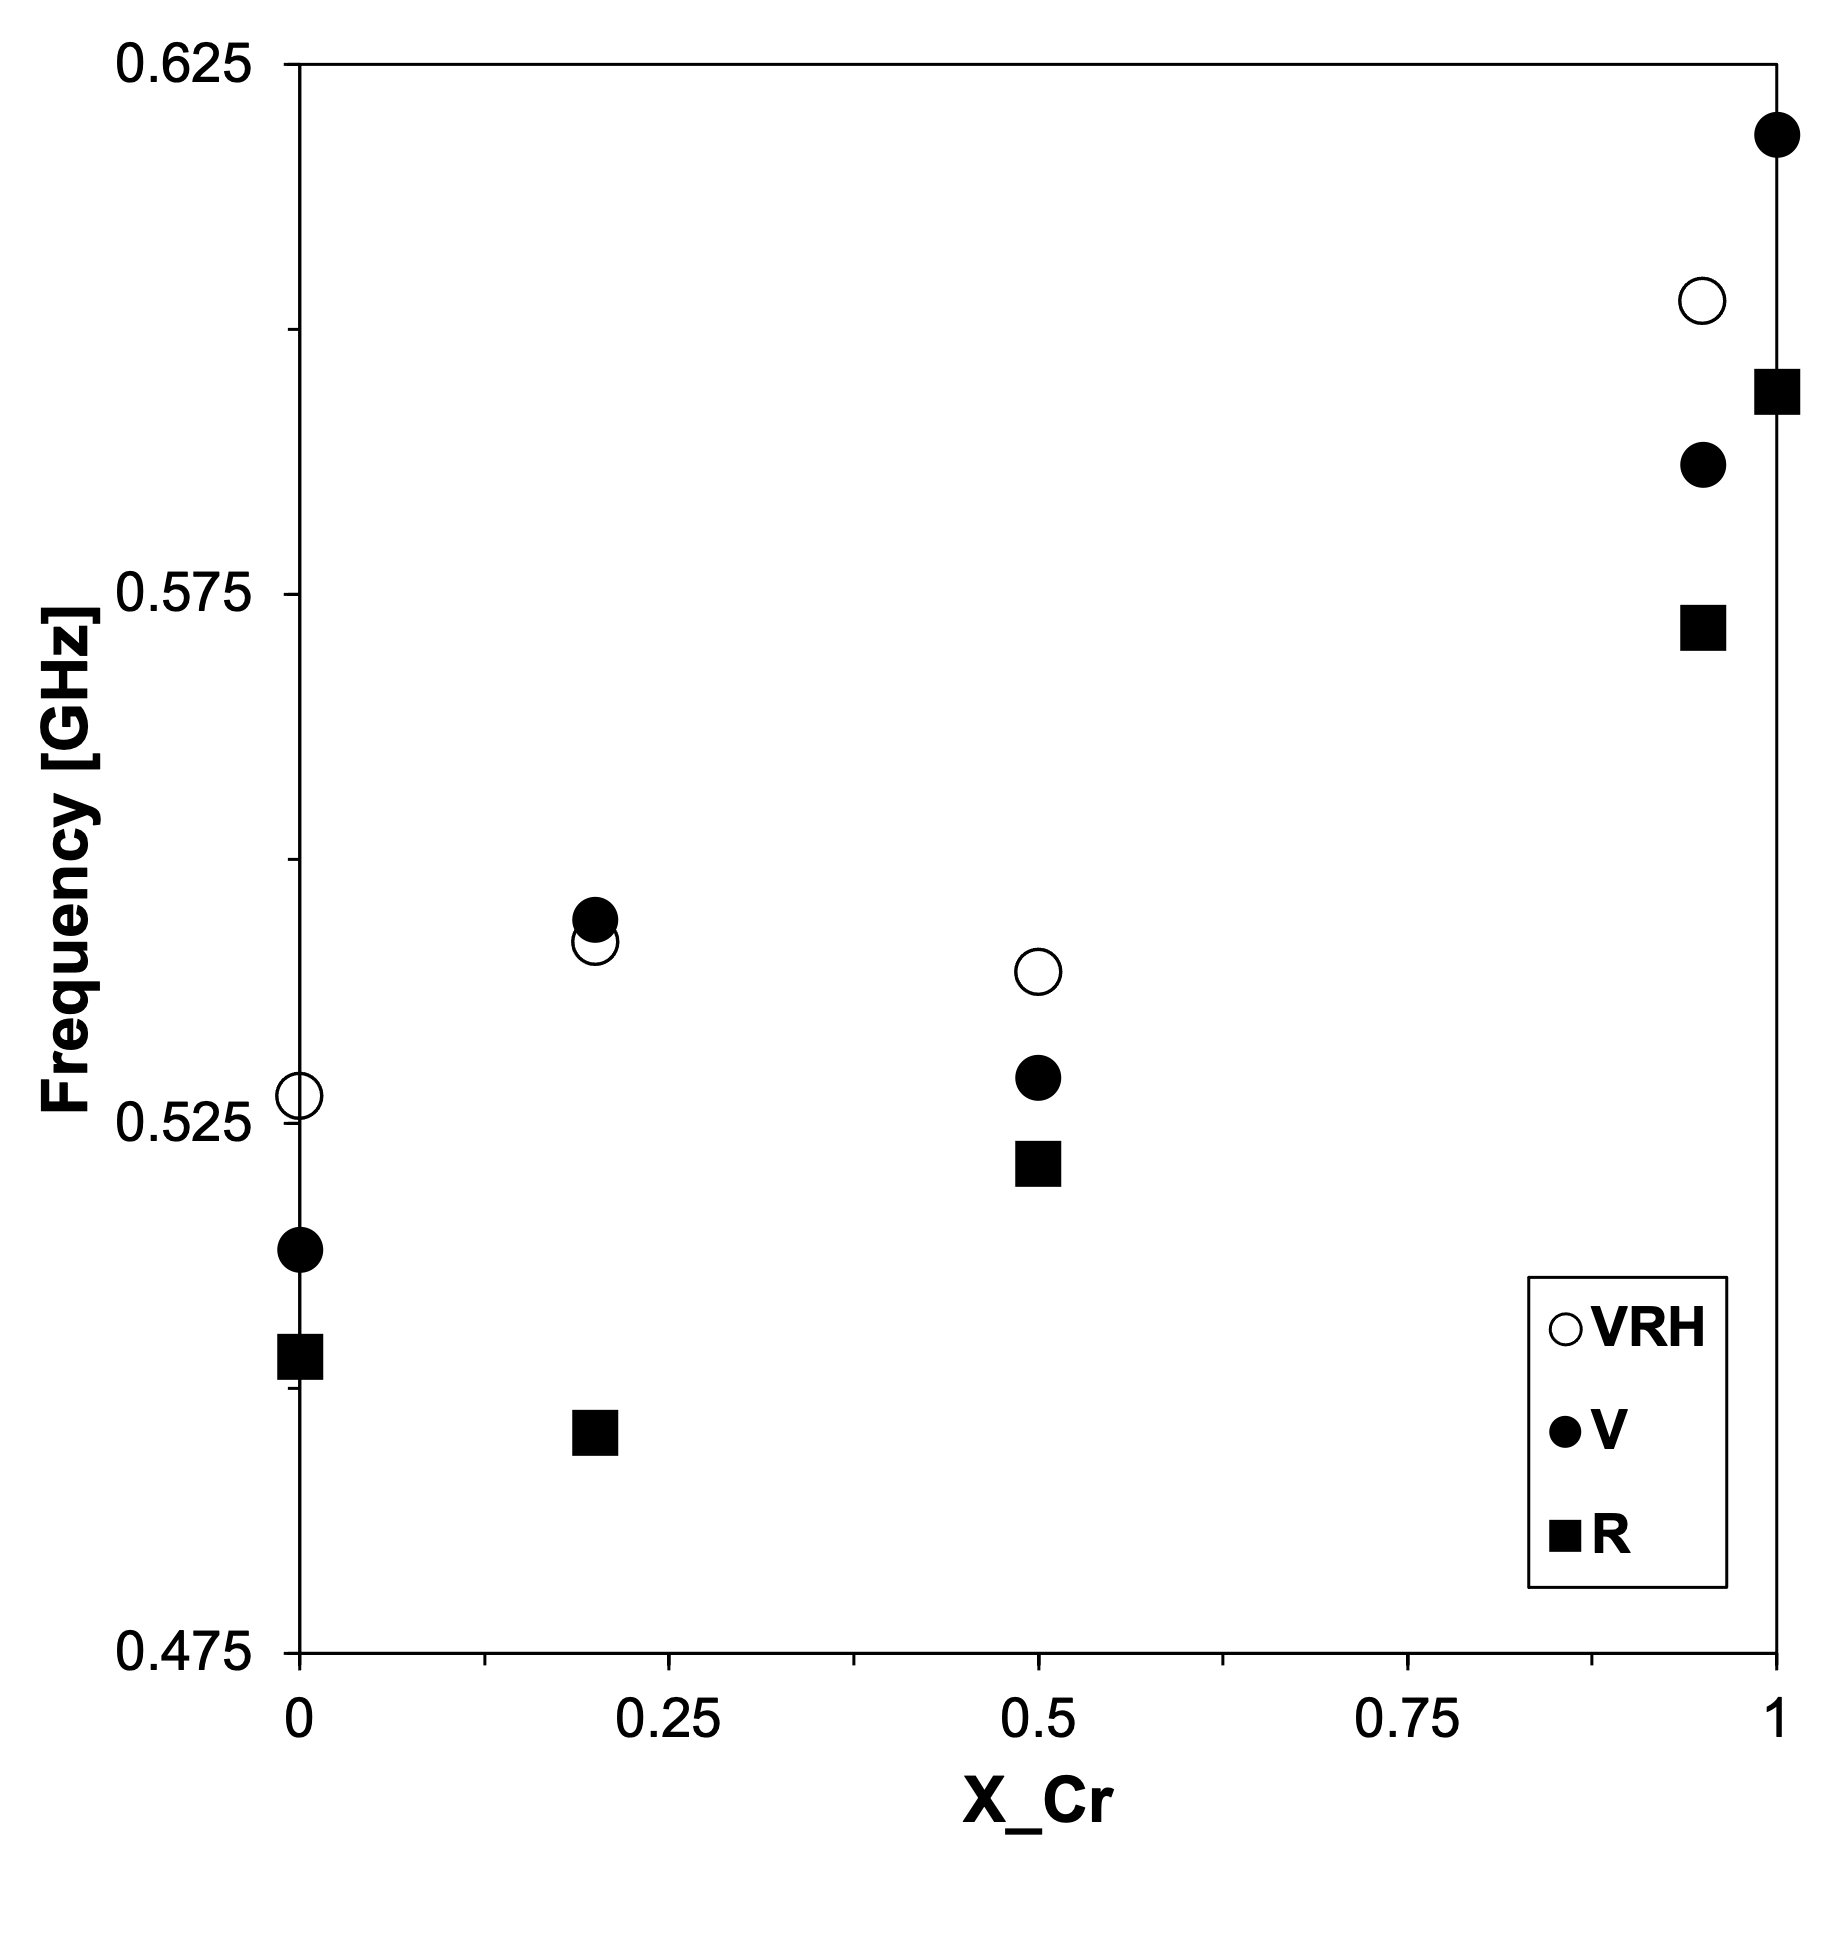
\includegraphics[width=\textwidth]{Parts/Figures/fvsX_v3.png}
        \caption{Calculated acoustic frequencies across different Cr compositions, illustrating the material's acoustic response variability with composition. This graph provides a quantitative measure of the material's mechanical behavior and its dependence on the microstructural characteristics induced by varying chromium content.}
        \label{fig4b}
    \end{subfigure}
    \begin{subfigure}{0.5\textwidth}
        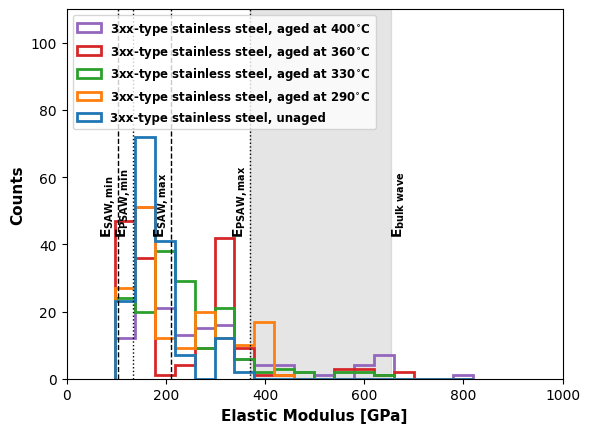
\includegraphics[width=\textwidth]{Parts/Figures/experimental-moduli-hist.png}
        \caption{Measured elastic moduli distribution from experimental data, highlighting the range and variability of material properties within stainless steel samples subjected to different thermal aging processes. The distribution underscores the significant impact of microstructural changes, such as spinodal decomposition, on the material's overall stiffness and mechanical integrity.}
        \label{fig4c}
    \end{subfigure}
    \caption{(a) Quantum elastodynamic frequencies obtained from density functional theory calculations reveal the complex interplay between microstructural evolution and mechanical properties in stainless steels undergoing spinodal decomposition. These findings are corroborated by (b) calculated acoustic frequencies that vary with Cr composition, providing a link between composition, microstructure, and acoustic properties. (c) The distribution of measured elastic moduli further validates the theoretical predictions, illustrating the broad impact of aging and compositional changes on the material's mechanical performance.}
    \label{fig4}
\end{sidewaysfigure}


\begin{sidewaysfigure}[!ht]
	\centering
	\begin{subfigure}{0.3\textwidth}
         \centering
         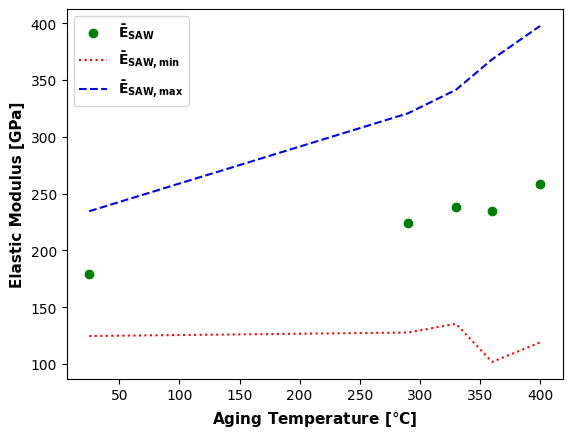
\includegraphics[width=\linewidth]{Parts/Figures/experimental-moduli-trend.png}
         \caption{Experimental elastic moduli of aged steels, displaying how aging temperature influences the material's stiffness. This graph illustrates the correlation between thermal treatment and the increase in elastic moduli, indicative of the material's response to microstructural changes over time.}
         \label{fig5a}
     \end{subfigure}
     \hfill
     \begin{subfigure}{0.3\textwidth}
         \centering
         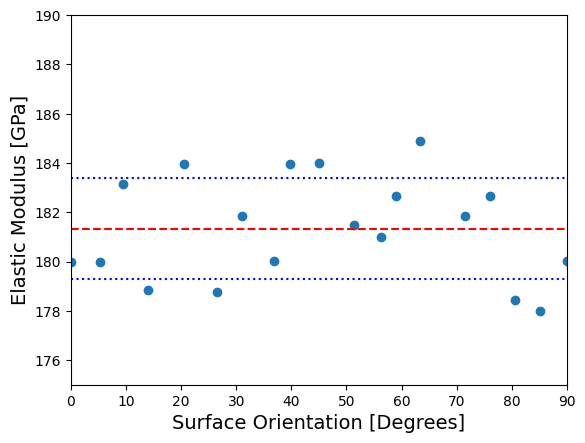
\includegraphics[width=\linewidth]{Parts/Figures/approximate-elastic-moduli-from-SAW-measurements-pristine.png}
         \caption{Theoretical elastic moduli of pristine steels, offering a baseline comparison for understanding how spinodal decomposition affects material properties before and after aging. This comparison elucidates the stiffening effect of microstructural evolution on the alloy's mechanical behavior.}
         \label{fig5b}
     \end{subfigure}
     \hfill
     \begin{subfigure}{0.3\textwidth}
         \centering
         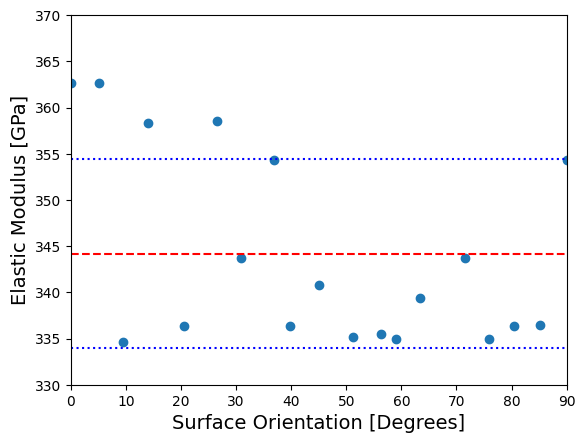
\includegraphics[width=\linewidth]{Parts/Figures/approximate-elastic-moduli-from-SAW-measurements-spindec.png}
         \caption{Theoretical elastic moduli of spinodally decomposed steels, demonstrating the pronounced impact of microstructural evolution on the alloy's stiffness. This direct comparison to pristine conditions highlights the significant role of chromium composition and thermal aging in material performance.}
         \label{fig5c}
     \end{subfigure}
     \hfill
     \begin{subfigure}{0.3\textwidth}
         \centering
         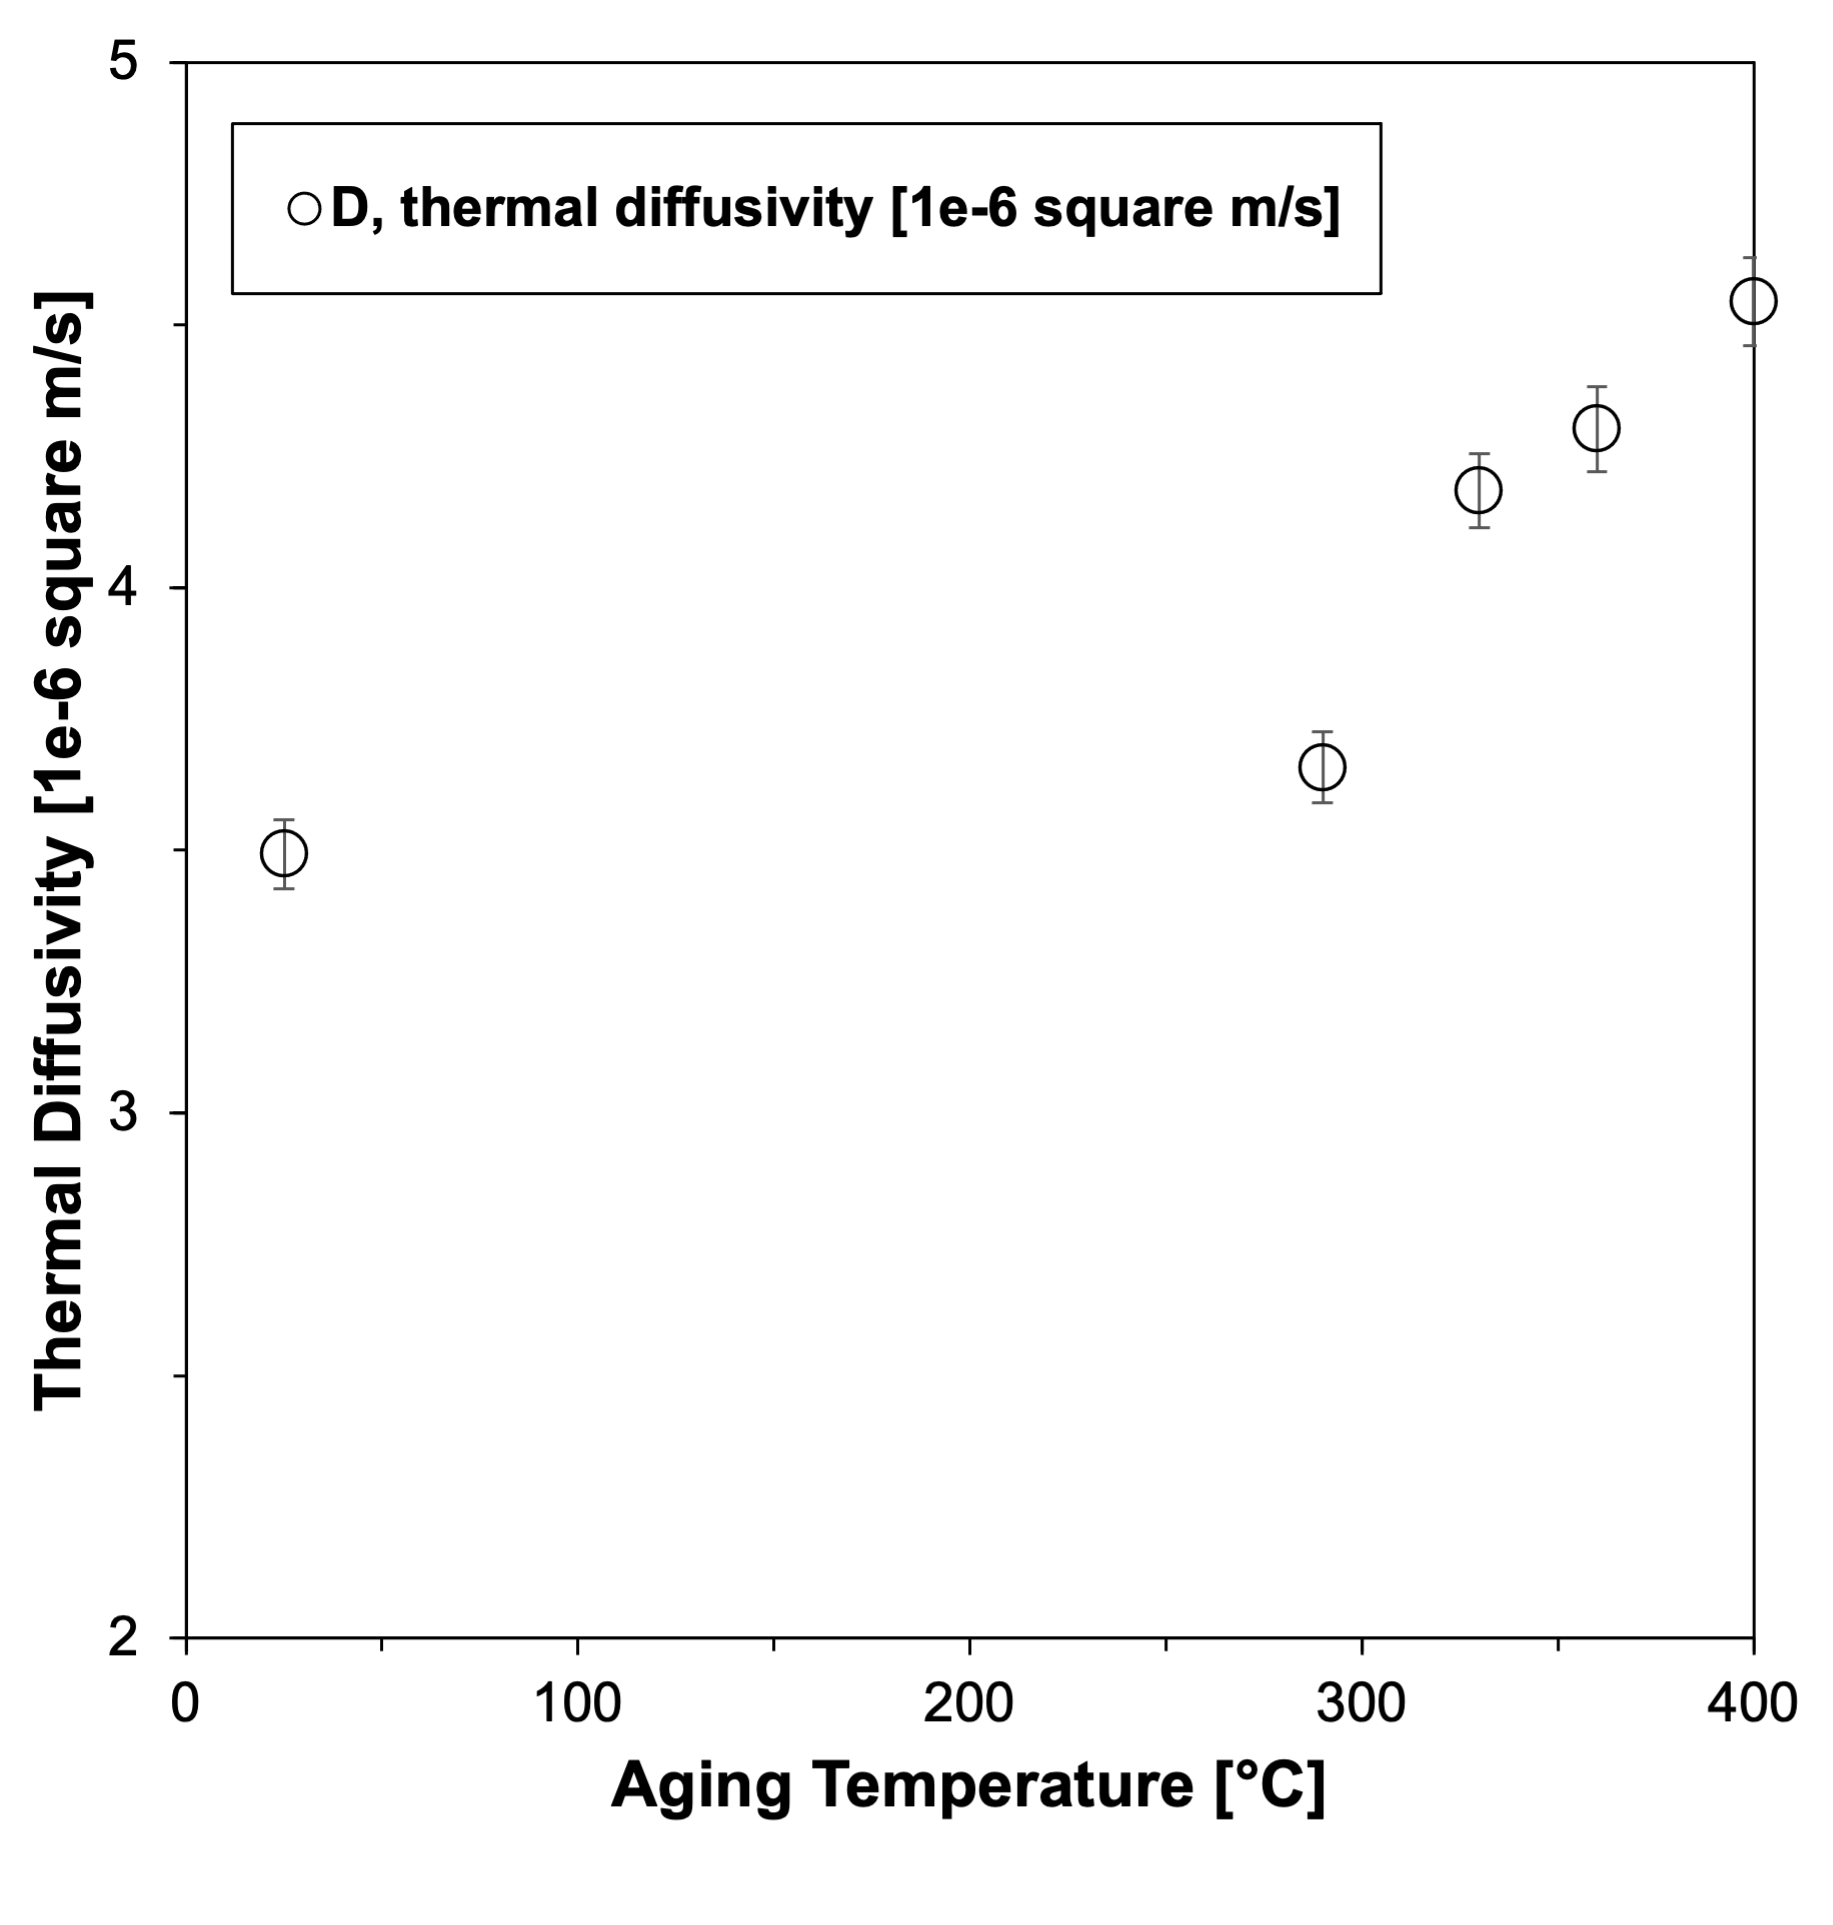
\includegraphics[width=\linewidth]{Parts/Figures/DvsT_CF8_30khrs_v2.png}
         \caption{\(D^{exp}_{thermal}\), experimental thermal diffusivity as measured in aged stainless steel, illustrating the thermal transport characteristics and their variation with temperature. This metric provides insights into the thermal stability and heat dissipation capabilities of the material post-aging.}
         \label{fig5d}
     \end{subfigure}
     \hfill
     \begin{subfigure}{0.3\textwidth}
         \centering
         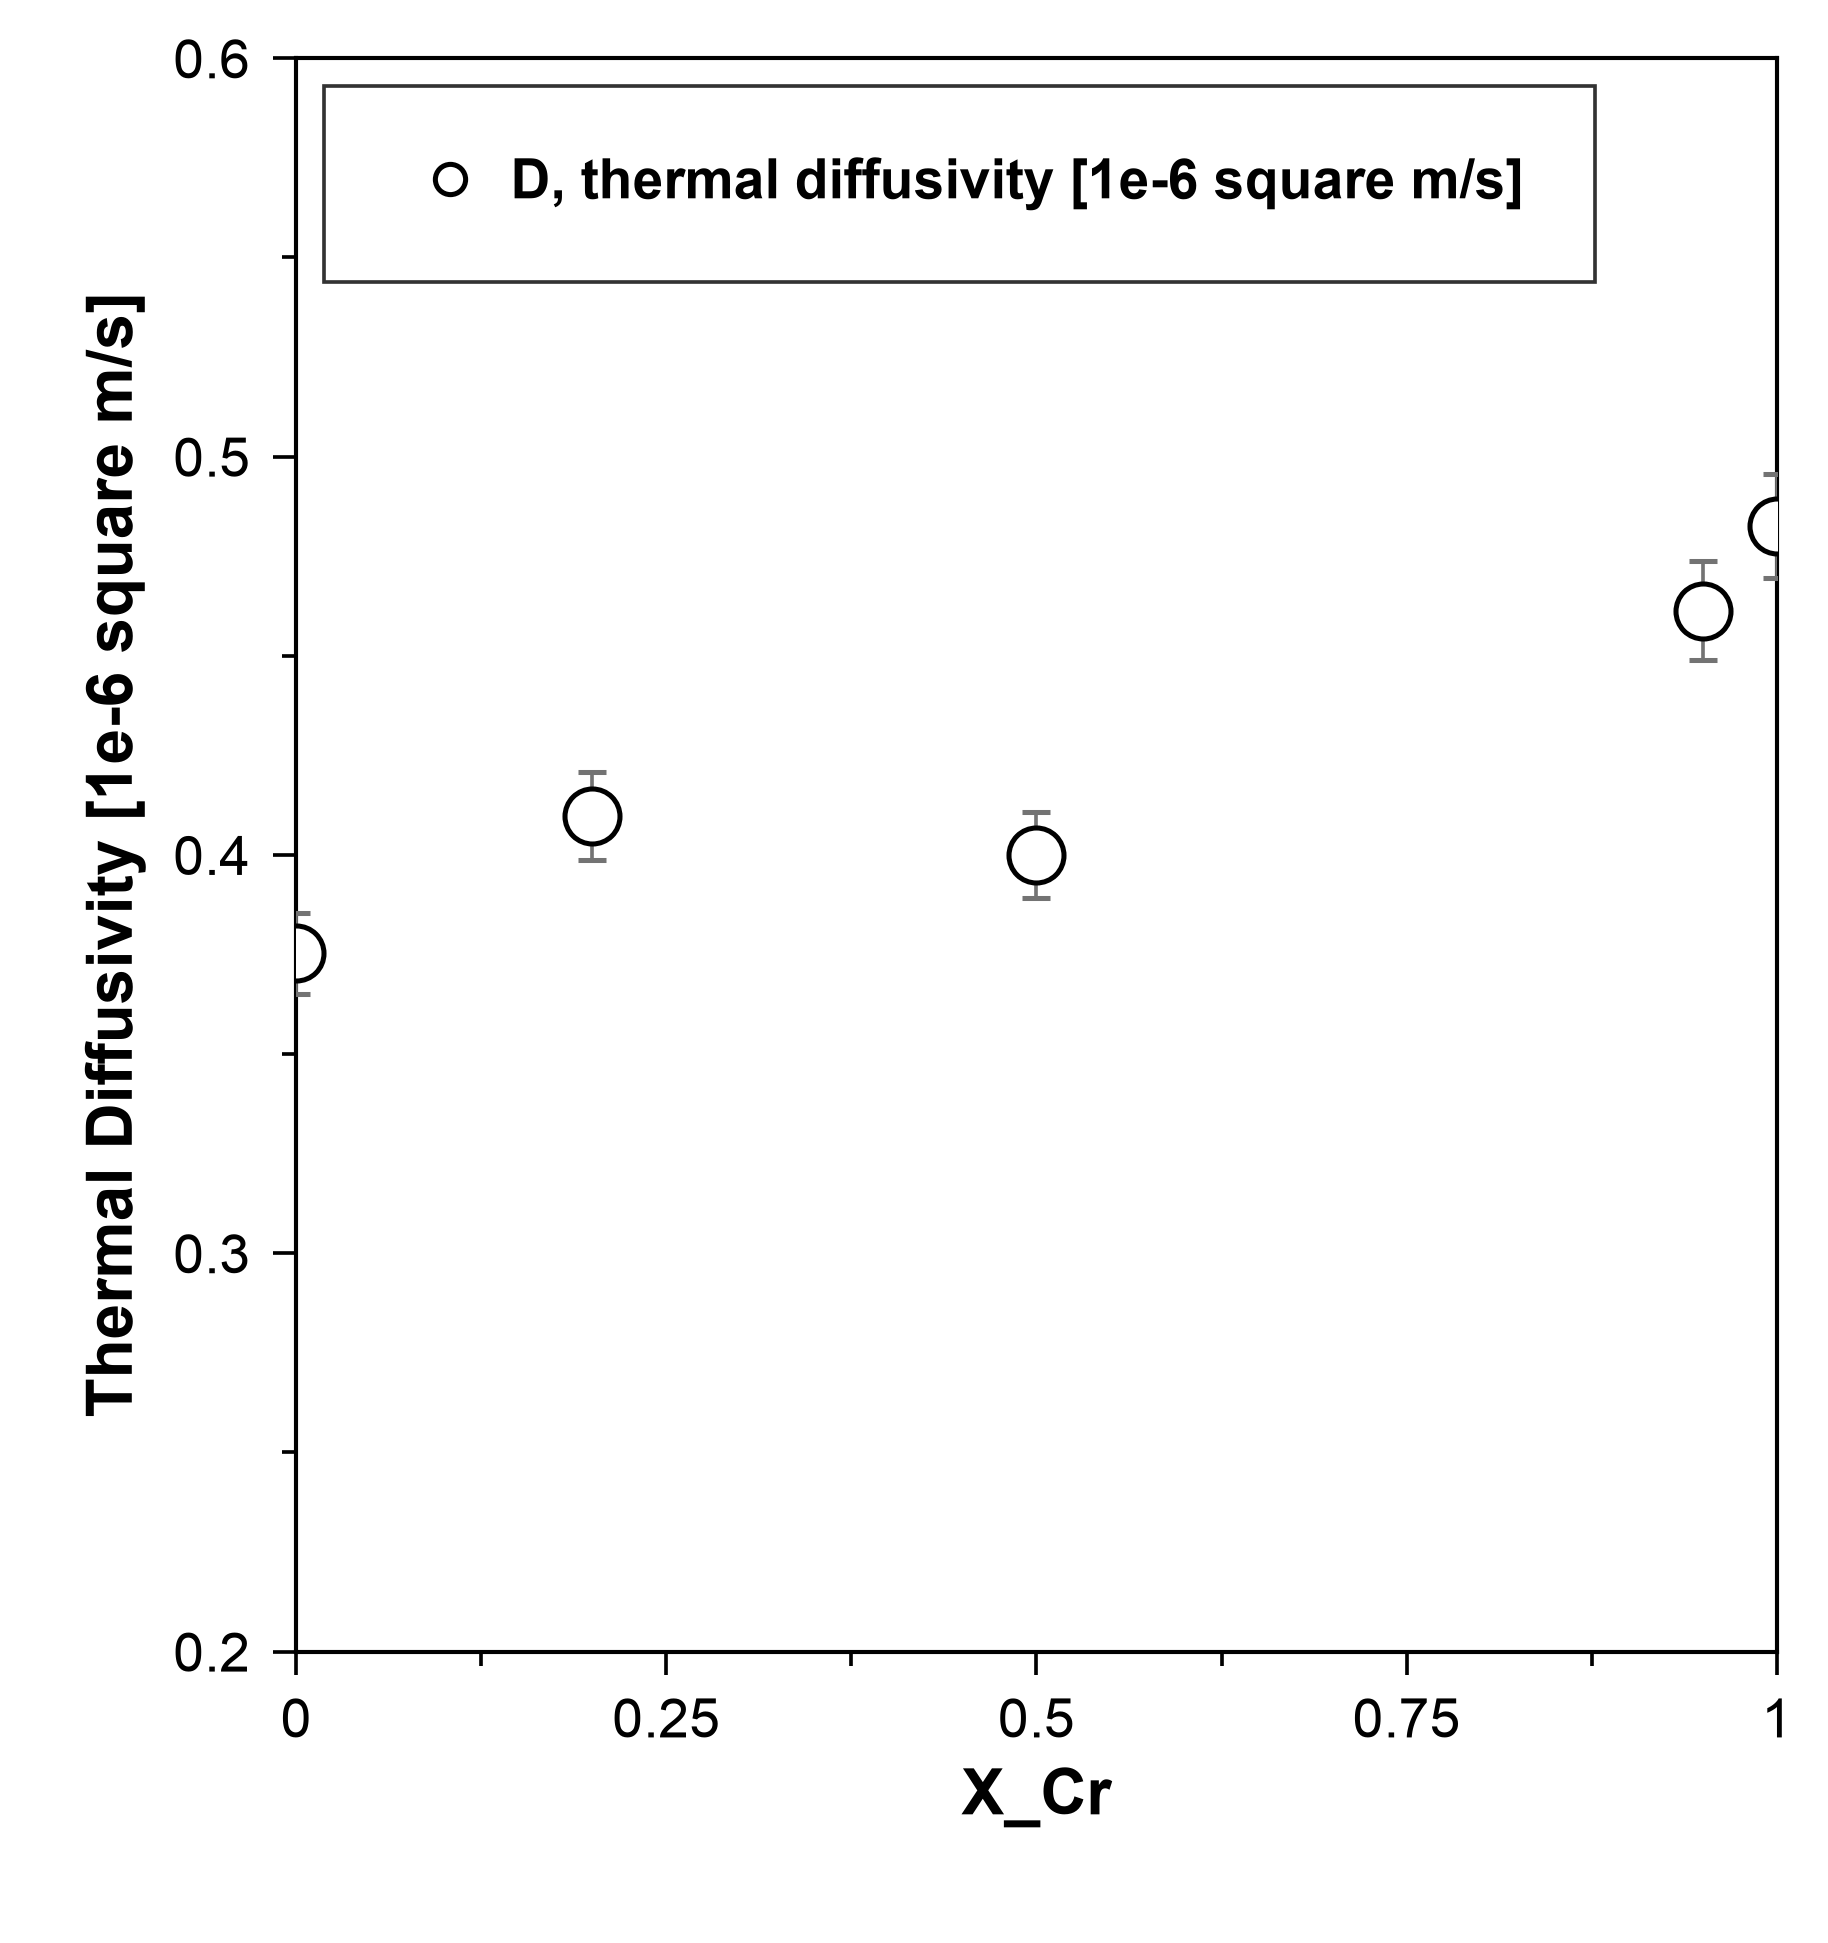
\includegraphics[width=\linewidth]{Parts/Figures/DvsX_v5.png}
         \caption{\(D^{theoretical}_{thermal}\), theoretical thermal diffusivity indicating the expected thermal behavior based on composition and microstructural considerations. This predictive analysis aids in understanding the thermal management potential of the alloy across a range of compositions.}
         \label{fig5e}
     \end{subfigure}
     \hfill
     \begin{subfigure}{0.3\textwidth}
         \centering
         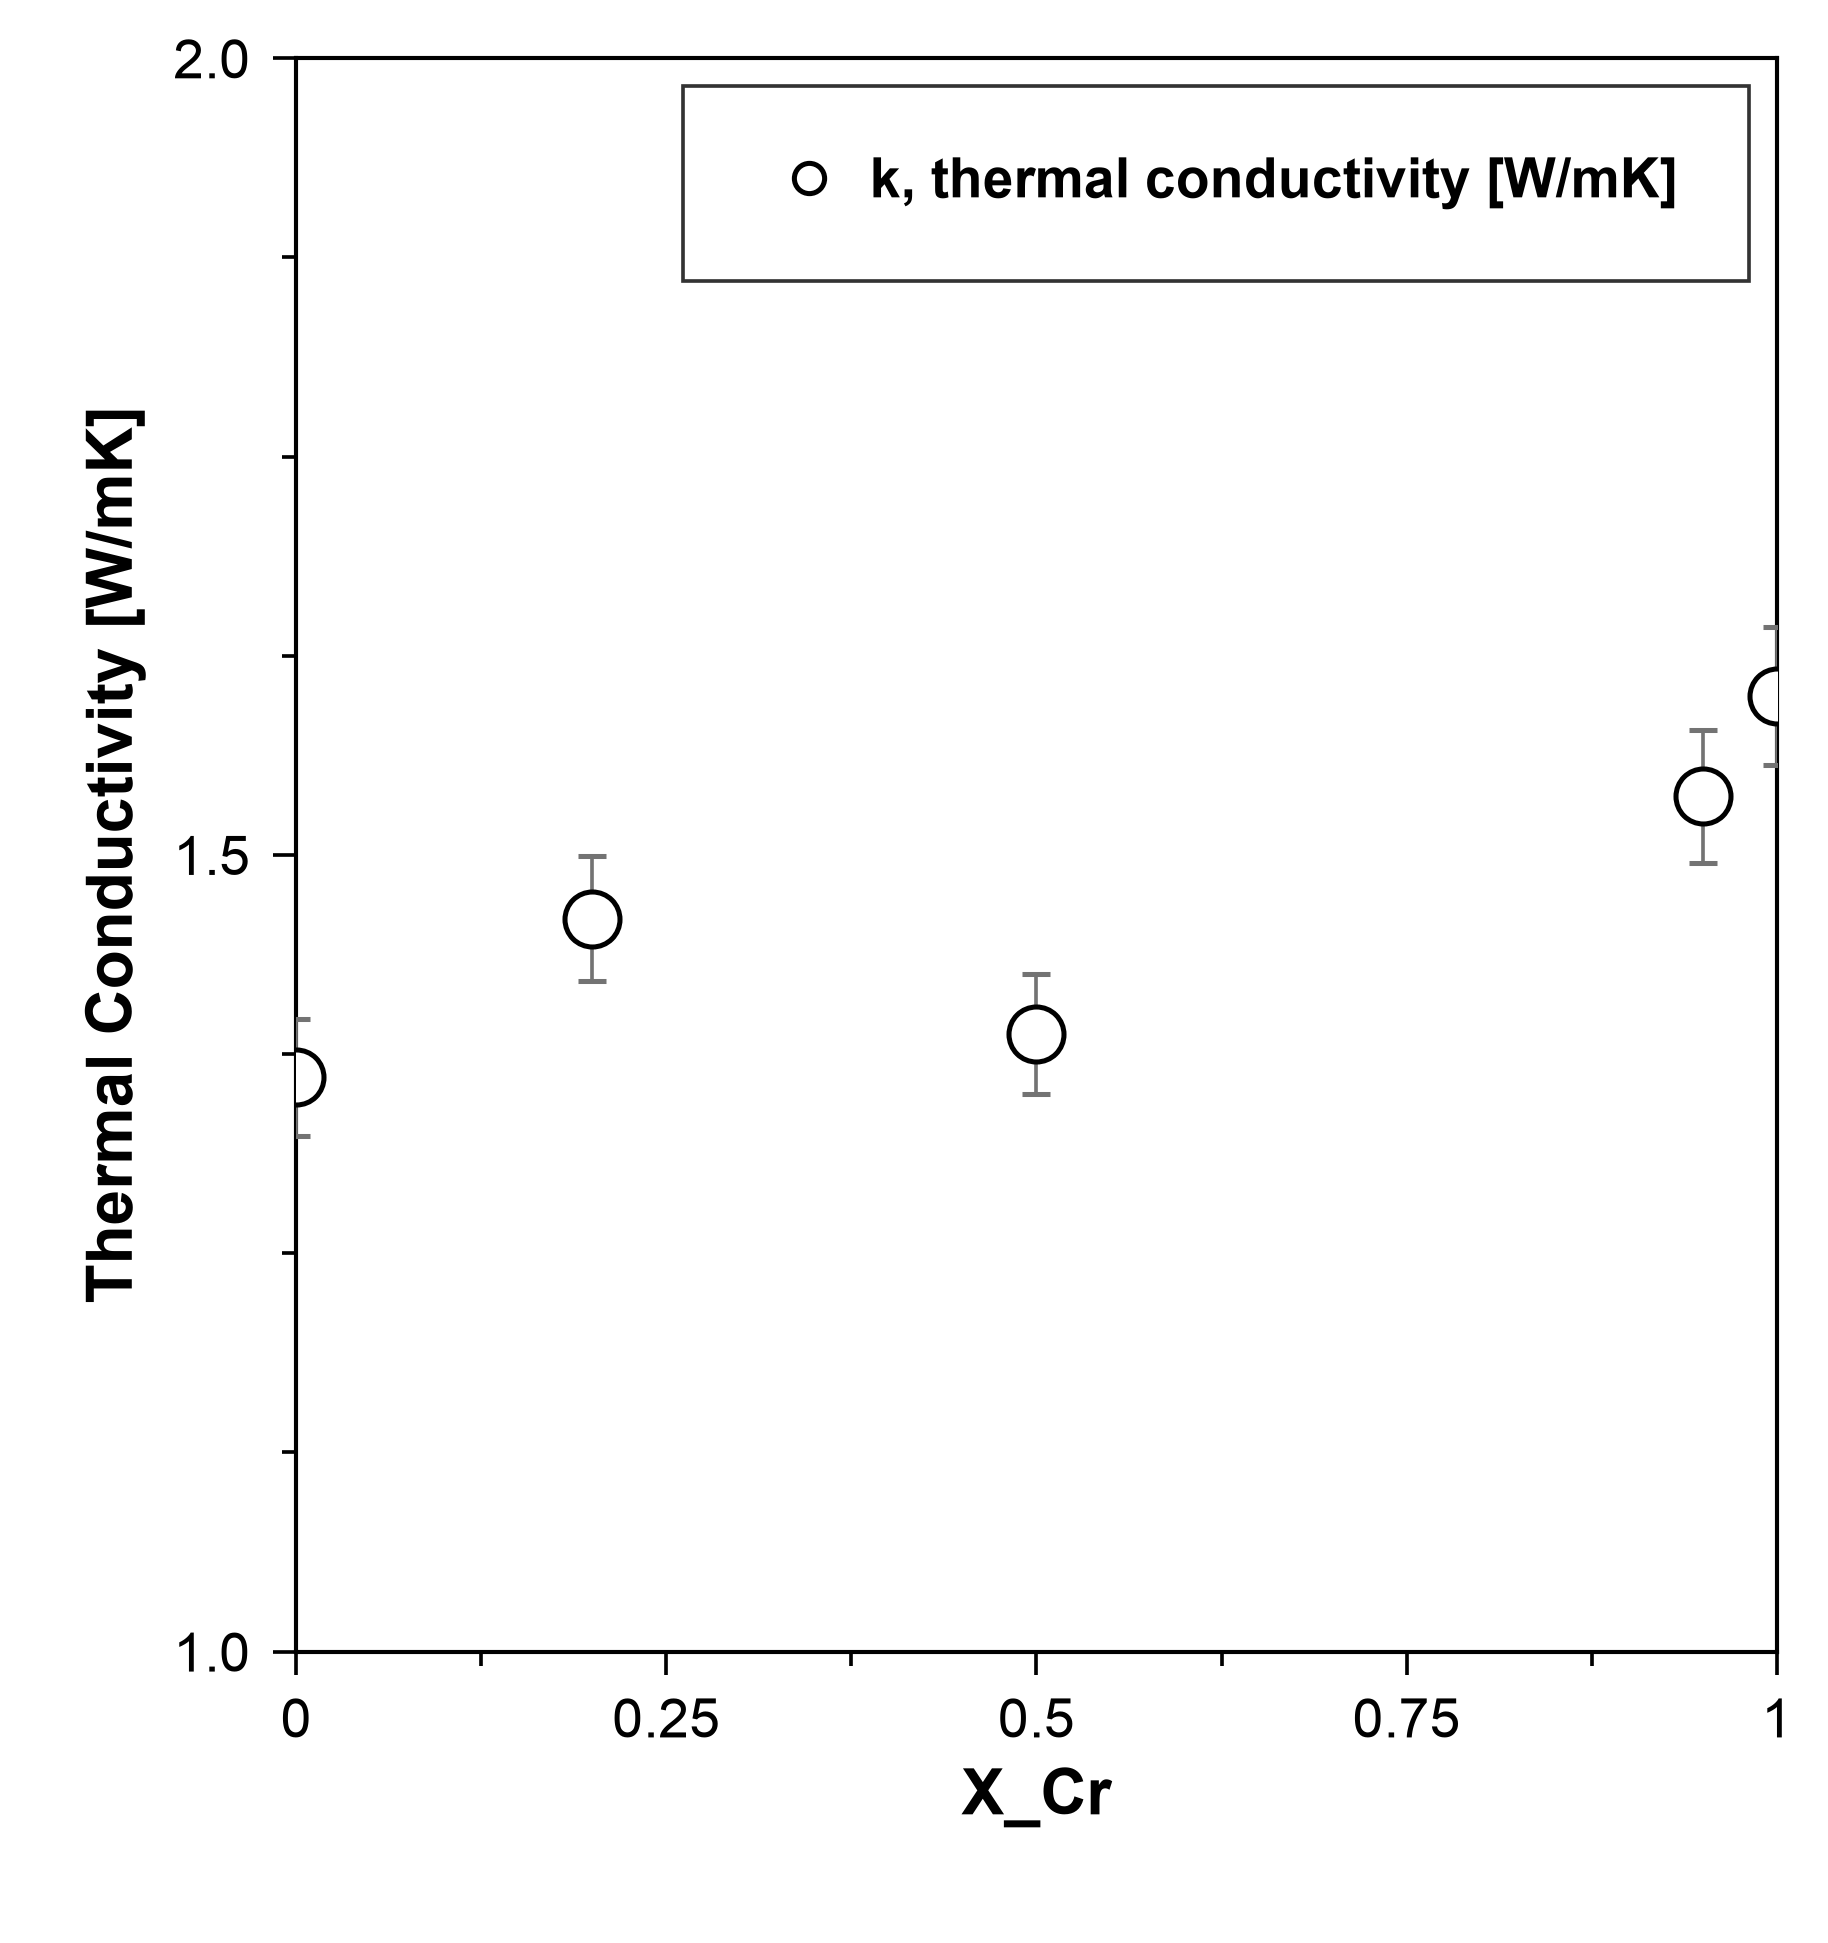
\includegraphics[width=\linewidth]{Parts/Figures/KvsX_v3.png}
         \caption{\(\kappa^{theoretical}_{thermal}\), thermal conductivity, showcasing the theoretical prediction of how efficiently the material conducts heat. This property is crucial for applications where thermal management is key, and it is influenced by the alloy's microstructure and composition.}
         \label{fig5f}
     \end{subfigure}
	\caption{Comprehensive analysis combining experimental and theoretical insights into the thermal and mechanical properties of stainless steels subjected to thermal aging. (a) Experimental elastic moduli trends with aging temperature highlight the stiffening effect of microstructural evolution. (b) and (c) Theoretical predictions for pristine and spinodally decomposed steels provide a comparative framework for assessing the impact of spinodal decomposition on material properties. (d) Experimental thermal diffusivity measurements, alongside (e) theoretical predictions for thermal diffusivity and (f) thermal conductivity, offer a holistic view of the material's thermal and mechanical behavior post-aging, emphasizing the interconnectedness of thermal properties, mechanical performance, and microstructural characteristics.}
	\label{fig5}
\end{sidewaysfigure}

\clearpage


\FloatBarrier
\clearpage
\subsection*{S3. First-principles calculations: methods and overview}
\paragraph{Methods.} An independent set of first-principles calculations was performed with Quantum ESPRESSO 7.5 \cite{giannozzi2009quantum,giannozzi2017advanced} on the MIT Engaging cluster, using PBE \cite{pbe1996} and PAW potentials from pslibrary (Fe 3s3p3d4s, Cr 3s3p3d4s), cutoffs of 60/480 Ry (wavefunctions/density), and Marzari--Vanderbilt smearing of 0.02 Ry. The alloys are 40-atom SQS ($2\times2\times5$ conventional \textit{bcc} cells; pair correlations optimised over three neighbour shells) at $x_{\mathrm{Cr}}$ from 0.05 to 0.95 (Table~\ref{tab:S_structural_convergence}), sampled with a $4\times4\times2$ $k$-mesh. Starting moments are ferromagnetic, except Cr antiparallel to Fe at 80\% Cr and for 65\% Cr at the experimental lattice parameter, which converge more reliably from that start, and each cell is fully relaxed (box lengths and ions). Elastic constants follow from the stress response to strains $\varepsilon_{xx}=\pm0.5\%$ and $\gamma_{yz}=\pm0.5\%$ with ions relaxed at each strain (central differences). For Fe--80Cr the SCF of the $-\varepsilon_{xx}$ step did not converge below $2\times10^{-6}$~Ry, and a rerun at that threshold shifts all diagonal stresses by 3~kbar (measured on the $\gamma_{yz}$ steps, which converged at both thresholds and give the same $C_{44}$ to 0.2~GPa). There $C_{11}$ and $C_{12}$ come from the forward difference between $+\varepsilon_{xx}$ and the relaxed cell. The response is linear: the relaxed shear stress lies at the midpoint of the $\pm\gamma_{yz}$ stresses to 0.005~kbar. Pure Fe (FM) and Cr (NM and commensurate AFM) use 2-atom cells with $16^3$ meshes. Convergence for \textit{bcc} Fe: $C_{ij}$ change by $\leq2$ GPa between 60 and 80 Ry and are converged by a $12^3$ mesh. Electronic structure: atom- and spin-projected DOS from a non-self-consistent $6\times6\times3$ run with the optimised tetrahedron method; Fermi-surface sections on the $k_z=0$ plane; band structures along $\Gamma$--H--N--$\Gamma$--P--H. Phonons: density-functional perturbation theory on a $6^3$ $q$-grid, Fourier-interpolated along the same path.

\paragraph{Overview.} The additional first-principles material is organised by topic: elastic constants at the PBE-relaxed and the room-temperature experimental lattice parameter (Section S4); electronic structure, including the unfolded Fermi surfaces and band structures of the Fe-rich alloys (S5); the electronic topological transition that links them to the Fe-rich elastic anomaly (S6); lattice dynamics (S7); a validation of every computed quantity against published data and experiment, including the thermal-transport estimates of Section S1 (S8); and the proposed mechanism figures (S9). Each section gives its text first and its figures after. The convergence of the elastic constants with Brillouin-zone sampling and cutoff is shown in Fig.~\ref{fig:S_convergence}, and the structural convergence of every relaxation (residual forces and pressures) in Table~\ref{tab:S_structural_convergence} and Fig.~\ref{fig:S_structural_convergence}.


\begin{figure}[!htbp]
\centering
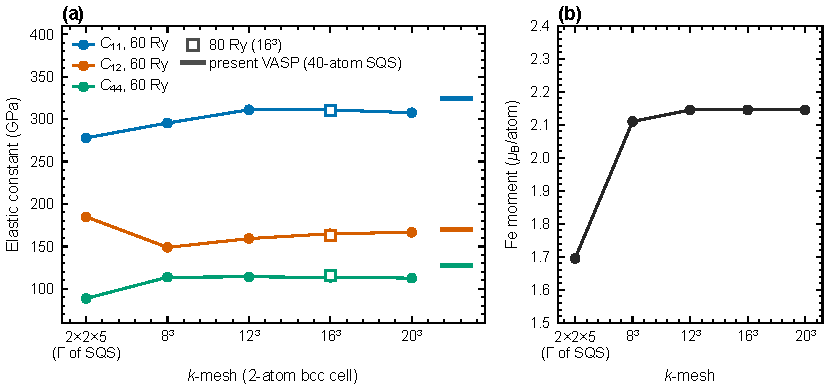
\includegraphics[width=0.85\textwidth]{figures/kdense_scripta/response/R_convergence.pdf}
\caption{Convergence of the Quantum ESPRESSO elastic constants of \textit{bcc} Fe (2-atom cell) with Brillouin-zone sampling. (a) $C_{11}$, $C_{12}$ and $C_{44}$ at 60~Ry from the $2\times2\times5$ mesh, which is equivalent to $\Gamma$-only sampling of the 40-atom SQS, to $20^3$; open squares, 80~Ry at $16^3$; bars at right, the present VASP tensor. (b) Fe moment for the same meshes.}
\label{fig:S_convergence}
\end{figure}

\begin{table}[!htbp]
\centering
\caption{Structural convergence of the Quantum ESPRESSO relaxations (40-atom SQS). Residual total force and pressure at
the last ionic step, and number of ionic (BFGS) steps. Thresholds: energy change $10^{-5}$~Ry, force components
$10^{-3}$~Ry/bohr, pressure 0.2~kbar for the PBE-relaxed cells; at the experimental lattice parameter the cell is fixed
and only the ions relax, hence the non-zero pressure. The SCF threshold is $10^{-8}$~Ry, except $3\times10^{-6}$~Ry for
the last 19 of the 21 ionic steps of Fe--65Cr at the experimental lattice parameter, where the SCF reached a $10^{-6}$~Ry noise floor (energy error below
1~$\mu$eV/atom). Every SCF of every ionic step converged.}
\label{tab:S_structural_convergence}
\small
\begin{tabular}{rlrrr}
\hline
$x_{\mathrm{Cr}}$ & lattice & force (Ry/bohr) & $P$ (kbar) & ionic steps \\
\hline
0.05 & relaxed & 0.0006 & -0.11 & 11 \\
0.10 & relaxed & 0.0013 & 0.00 & 9 \\
0.20 & relaxed & 0.0019 & 0.04 & 12 \\
0.30 & relaxed & 0.0008 & -0.12 & 16 \\
0.35 & relaxed & 0.0015 & 0.12 & 12 \\
0.40 & relaxed & 0.0020 & 0.12 & 9 \\
0.45 & relaxed & 0.0011 & -0.07 & 16 \\
0.475 & relaxed & 0.0010 & -0.08 & 16 \\
0.50 & relaxed & 0.0021 & -0.10 & 13 \\
0.65 & relaxed & 0.0014 & -0.10 & 15 \\
0.70 & relaxed & 0.0011 & -0.07 & 16 \\
0.95 & relaxed & 0.0006 & 0.05 & 9 \\
0.05 & exp. & 0.0014 & -63.05 & 9 \\
0.10 & exp. & 0.0016 & -66.28 & 9 \\
0.20 & exp. & 0.0017 & -59.98 & 14 \\
0.30 & exp. & 0.0010 & -71.41 & 17 \\
0.35 & exp. & 0.0017 & -74.33 & 11 \\
0.40 & exp. & 0.0023 & -75.47 & 9 \\
0.45 & exp. & 0.0013 & -80.61 & 17 \\
0.50 & exp. & 0.0017 & -83.82 & 15 \\
0.65 & exp. & 0.0030 & -91.64 & 21 \\
0.80 & exp. & 0.0020 & -69.40 & 12 \\
0.95 & exp. & 0.0008 & -101.31 & 8 \\
\hline
\end{tabular}
\end{table}


\begin{figure}[!htbp]
\centering
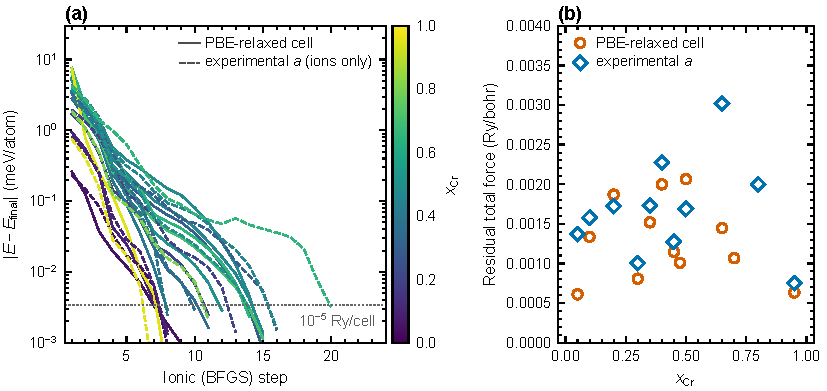
\includegraphics[width=0.85\textwidth]{figures/kdense_scripta/response/R_structural_convergence.pdf}
\caption{Structural convergence of the Quantum ESPRESSO relaxations of Table~\ref{tab:S_structural_convergence}. (a) Total energy relative to its final value against ionic (BFGS) step, coloured by $x_{\mathrm{Cr}}$; solid, PBE-relaxed cell; dashed, experimental lattice parameter with ions relaxed. Dotted line: the $10^{-5}$~Ry energy threshold per 40-atom cell. Resumed runs are shown as one continuous sequence. (b) Residual total force at the last ionic step.}
\label{fig:S_structural_convergence}
\end{figure}

\FloatBarrier
\clearpage
\subsection*{S4. Elastic constants}
Figure~\ref{fig:S_fe_rich} compares the Fe-rich elastic constants with EMTO-CPA and MD. Figure~\ref{fig:S_qe_aexp} repeats the QE calculations at the room-temperature experimental lattice parameter (Vegard between Fe 2.8665 and Cr 2.8846~\AA; cubic cell fixed, ions relaxed), the convention of the EMTO-CPA reference data \cite{razumovskiy2011first}. PBE relaxes all compositions to about 11.4~\AA$^3$/atom, about 4\% below experiment; the bulk modulus is the property most sensitive to this (Section S8).

At the experimental lattice parameter $f_{\mathrm{SAW}}$ rises from 446~MHz for Fe (EMTO-CPA: 449~MHz) to 485 at 20\%, flattens at 497, 500 and 499~MHz between 30 and 40\%~Cr (EMTO-CPA: 503, 488, 490~MHz), and reaches 513 at 50\% (513), 542 at 80\% and 580~MHz for AFM Cr (602). The bulk modulus has a local minimum at 40\%~Cr (163~GPa) where the Cr moments collapse, and the shear modulus flattens there. The experimental lattice parameter thus reproduces the magnitude of $f_{\mathrm{SAW}}$ and a magnetic anomaly near Fe--36Cr, but not the Fe-rich maximum near 20\%~Cr of the EMTO-CPA curve, so it gives a plateau rather than a minimum. At the PBE-relaxed volume $f_{\mathrm{SAW}}$ rises steadily from 504 to 591~MHz. The bulk-modulus drops at 80\% and 100\%~Cr reflect antiferromagnetic (Cr) and ferrimagnetic (Fe--80Cr, Cr antiparallel to Fe, net 0.31~$\mu_{\mathrm B}$/atom) order, which collapses $C_{12}$ as in pure Cr.

\begin{figure}[!htbp]
\centering
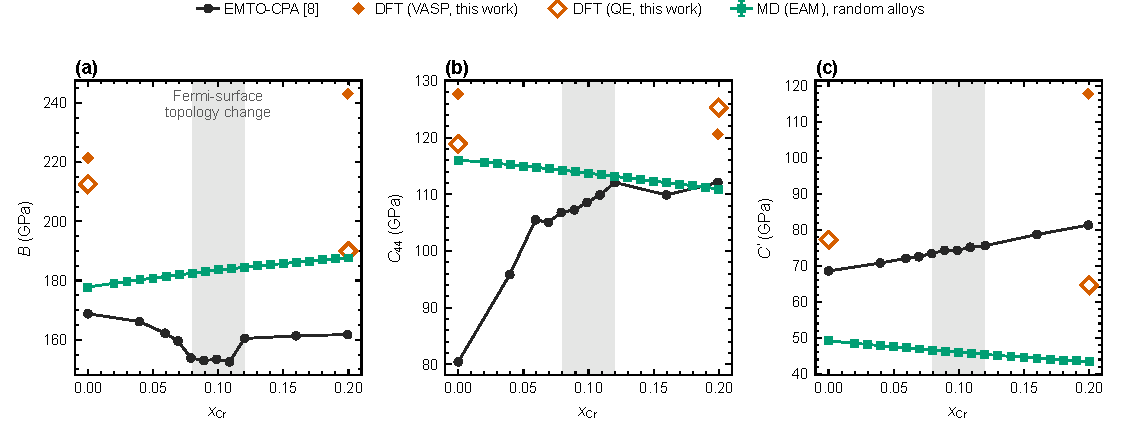
\includegraphics[width=\textwidth]{figures/kdense_scripta/supplementary/S_fe_rich_elastic.pdf}
\caption{Fe-rich elastic constants ($x_{\mathrm{Cr}}\leq0.2$): bulk modulus $B$, $C_{44}$ and $C'$ from EMTO-CPA \cite{razumovskiy2011first}, MD (EAM) random alloys on a 1\% composition grid, and the present VASP and Quantum ESPRESSO calculations. Validation against measured bulk moduli (compiled in Ref.~\cite{korzhavyi2009electronic}): at the relaxed PBE volume both DFT codes overestimate $B$ (VASP: Fe 221 vs 168 GPa, $+32\%$; QE SQS at 95\% Cr: $+31\%$ against the paramagnetic value), the usual consequence of the too-small PBE volume of Fe--Cr; at the room-temperature experimental lattice parameter the QE value at 95\% Cr is within 7\%. The shaded band (0.08--0.12) marks the composition range of the Fermi-surface topology change reported in Ref.~\cite{razumovskiy2011first}; the classical potential has no electronic structure and does not reproduce it.}
\label{fig:S_fe_rich}
\end{figure}

\begin{figure}[!htbp]
\centering
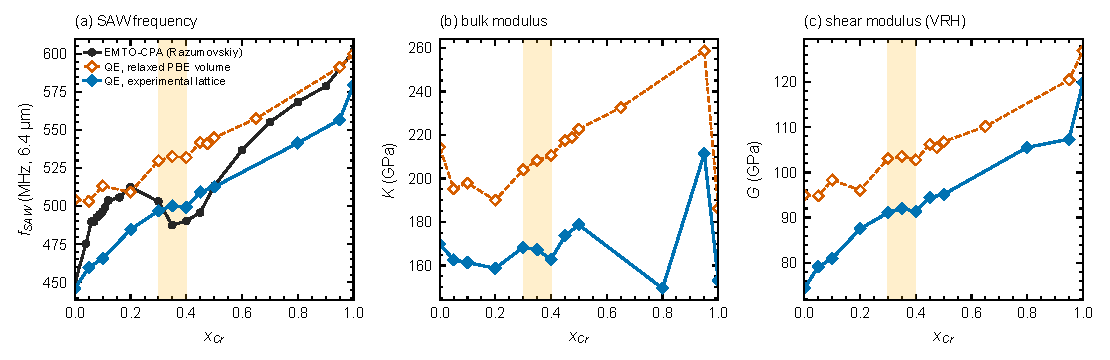
\includegraphics[width=\textwidth]{figures/kdense_scripta/supplementary/S_qe_aexp_progress.pdf}
\caption{QE 40-atom SQS and pure elements at the PBE-relaxed (open, dashed) and the room-temperature experimental (filled) lattice parameter, against EMTO-CPA \cite{razumovskiy2011first}: (a) $f_{\mathrm{SAW}}$ at $\lambda=6.4\,\mu$m, (b) bulk modulus, (c) VRH shear modulus. The shaded band marks 30--40\%~Cr. Pure Cr is AFM; Fe--80Cr at the experimental lattice parameter converged to a ferrimagnetic state.}
\label{fig:S_qe_aexp}
\end{figure}

\textit{Spinodal window from the QE enthalpies.} The complete QE enthalpies of mixing (Fig.~\ref{fig:free_energy}a) can be fitted with Redlich--Kister polynomials, $\Delta H_{\mathrm{mix}}=x(1-x)\sum_k L_k(1-2x)^k$, and combined with the ideal configurational entropy to give the demixing curvature (Fig.~\ref{fig:S_qe_spinodal}). With four terms (RMS 2.3 and 4.2 meV/atom at the PBE-relaxed and experimental lattice parameters) the alloy is unstable at 748~K for $0.24\leq x_{\mathrm{Cr}}\leq0.99$ and $0.23\leq x_{\mathrm{Cr}}\leq0.99$, respectively. With three terms (RMS 3.8 and 6.2 meV/atom) the window is 0.34--0.96 and 0.36--0.97, which places Fe--36Cr on its lower edge. The lower edge therefore depends on the fit and is not determined by the present data to better than about 0.1. The upper edge lies far above the CALPHAD value of 0.71 \cite{xiong2011improved} because these are 0~K ferromagnetic energies, which omit the paramagnetism of Cr-rich alloys at the aging temperature. We therefore keep the CALPHAD window (0.30--0.71 at 748~K) as the reference in the main text and use the QE enthalpies only for the shape of $\Delta G_{\mathrm{demix}}$ in Fig.~\ref{fig:free_energy}a.

\begin{figure}[!htbp]
\centering
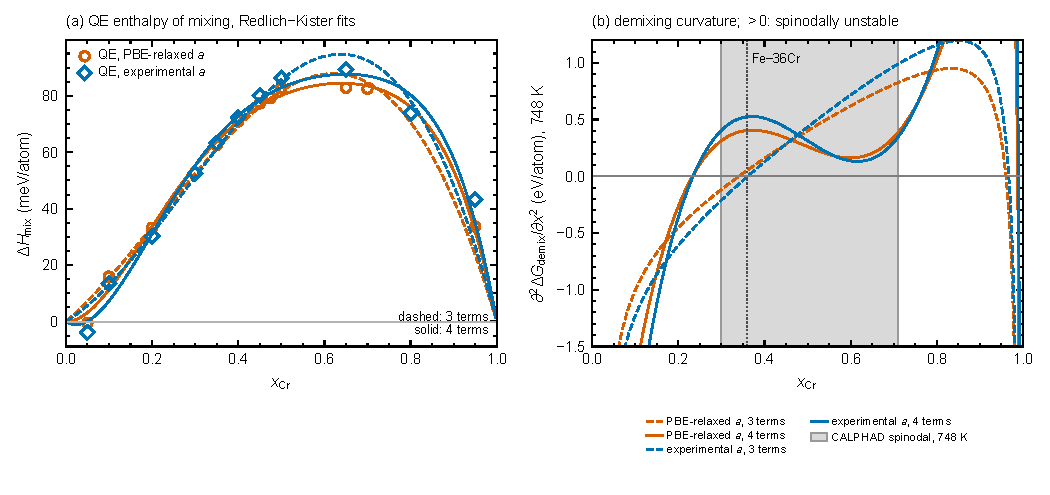
\includegraphics[width=\textwidth]{figures/kdense_scripta/supplementary/S_qe_spinodal.pdf}
\caption{Spinodal window implied by the QE enthalpies of mixing. (a) QE $\Delta H_{\mathrm{mix}}$ of the 40-atom SQS at the PBE-relaxed (circles) and experimental (diamonds) lattice parameter, with three-term (dashed) and four-term (solid) Redlich--Kister fits. (b) Demixing curvature $\partial^2\Delta G_{\mathrm{demix}}/\partial x^2$ at 748~K from each fit with the ideal configurational entropy; positive values are spinodally unstable. Grey band: CALPHAD chemical spinodal at 748~K \cite{xiong2011improved}; dotted line: Fe--36Cr. The lower edge of the QE window moves from 0.23 to 0.34--0.37 with the fit order; the upper edge (0.96--0.99) reflects the 0~K ferromagnetic reference. Script: \texttt{scripts/make\_qe\_spinodal\_sm.py}.}
\label{fig:S_qe_spinodal}
\end{figure}

\paragraph{MD checks.} The $25^3$-cell MD procedure reproduces the published $50^3$ series at Fe$_{50}$Cr$_{50}$, and the new random alloys reproduce its random-alloy $C_{11}$ (Fig.~\ref{fig:S_md_validation}). Full decomposition stiffens the MD alloys most inside the spinodal window, and no MD tensor, random or decomposed, reaches the unallowed band (Fig.~\ref{fig:S_md_decomposition}).

\begin{figure}[!htbp]
\centering
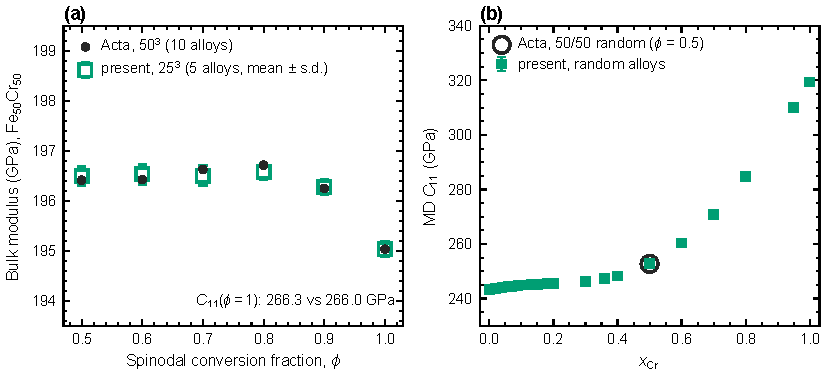
\includegraphics[width=0.85\textwidth]{figures/kdense_scripta/response/R_md_validation_v2.pdf}
\caption{Validation of the MD procedures against Ref.~\cite{al2023detecting}. (a) Bulk modulus of Fe$_{50}$Cr$_{50}$ against spinodal conversion fraction: the published $50^3$ series (10 alloys) and the present $25^3$ series (5 alloys, mean $\pm$ s.d.); $C_{11}$ at $\phi=1$ is 266.3 against 266.0~GPa. (b) $C_{11}$ of the present MD random alloys across composition, with the published equiatomic random-alloy value.}
\label{fig:S_md_validation}
\end{figure}

\begin{figure}[!htbp]
\centering
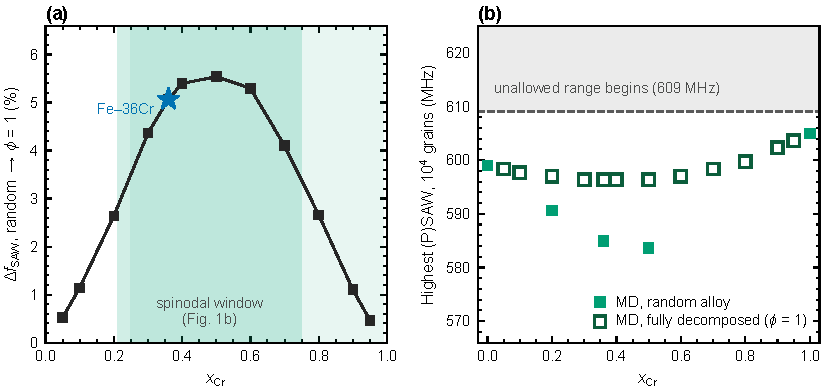
\includegraphics[width=0.85\textwidth]{figures/kdense_scripta/response/R_decomposition.pdf}
\caption{MD stiffening on full decomposition across composition ($25^3$ cells, five alloys per composition). (a) Relative change of $f_{\mathrm{SAW}}$ between the random ($\phi=0.5$) and fully decomposed ($\phi=1$) states at twelve compositions, with the spinodal windows shaded. (b) Highest (P)SAW frequency over $10^4$ grains for the random and decomposed MD tensors: decomposition never reaches the unallowed band.}
\label{fig:S_md_decomposition}
\end{figure}

\FloatBarrier
\clearpage
\subsection*{S5. Electronic structure}
Fermi surfaces and band structures of the pure metals (Figs.~\ref{fig:S_fermi_Fe}--\ref{fig:S_bands_aexp}) set the reference for the alloys. The unfolded Fermi surfaces and band structures of the Fe-rich SQS (Figs.~\ref{fig:S_fermi_unfolded} and \ref{fig:S_bands_unfolded}) follow how Cr changes the spin-up Fermi surface; the projected densities of states of the SQS (Fig.~\ref{fig:S_dos}) show the composition dependence of the Fe and Cr states and of the Fermi-level DOS.

\begin{figure}[!htbp]
\centering
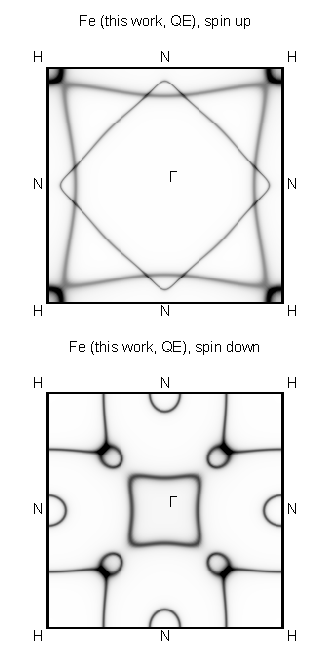
\includegraphics[width=0.42\textwidth]{figures/kdense_scripta/supplementary/S_fermi_Fe.pdf}
\caption{Fermi surface of ferromagnetic \textit{bcc} Fe in the (001) plane through $\Gamma$ (square with H at the corners), spin up and spin down, shown as a broadened spectral function in the layout of Korzhavyi \textit{et al.}\ \cite{korzhavyi2009electronic} (their Fig.~6).}
\label{fig:S_fermi_Fe}
\end{figure}

\begin{figure}[!htbp]
\centering
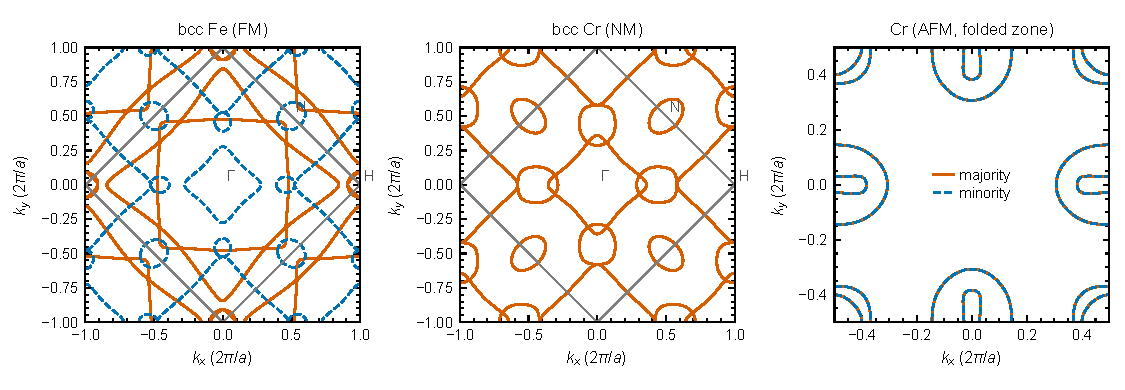
\includegraphics[width=\textwidth]{figures/kdense_scripta/supplementary/S_fermi_pure.pdf}
\caption{Fermi-surface sections ($k_z=0$) of \textit{bcc} Fe (FM; solid, majority; dashed, minority), \textit{bcc} Cr (NM) and commensurate AFM Cr (folded simple-cubic zone; both spin channels coincide). The nested electron and hole sheets of Cr are responsible for its incommensurate spin-density wave.}
\label{fig:S_fermi_pure}
\end{figure}

\begin{figure}[!htbp]
\centering
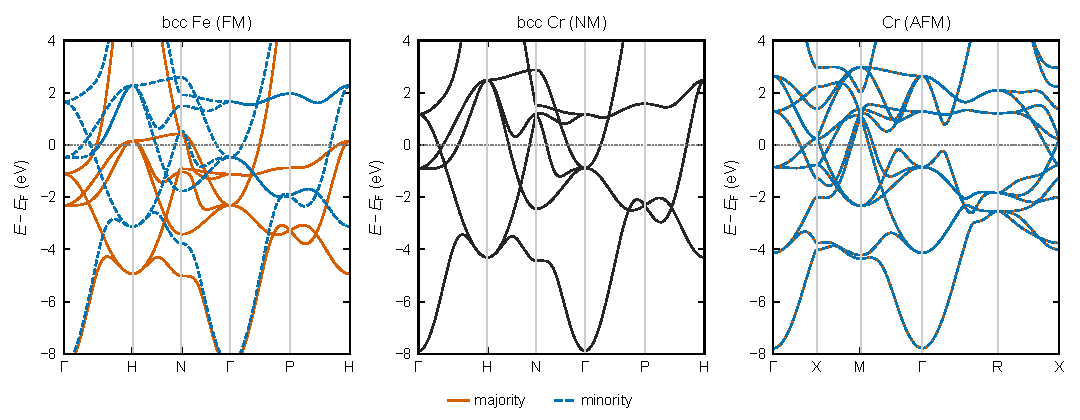
\includegraphics[width=\textwidth]{figures/kdense_scripta/supplementary/S_bands_pure_v2.pdf}
\caption{Electronic band structures of \textit{bcc} Fe (FM), \textit{bcc} Cr (NM) and AFM Cr (simple-cubic path), Quantum ESPRESSO. Validation: along $\Gamma$--H the Fe bands within $\pm2.7$ eV of $E_{\mathrm F}$ agree with the EMTO-CPA spectrum of pure Fe (Korzhavyi \textit{et al.}\ \cite{korzhavyi2009electronic}, Fig.~7) to an RMS of 0.22 eV (spin up) and 0.17 eV (spin down); the band crossings at $E_{\mathrm F}$ and the H-point level 0.15 eV above $E_{\mathrm F}$ in the majority channel coincide.}
\label{fig:S_bands_pure}
\end{figure}

\begin{figure}[!htbp]
\centering
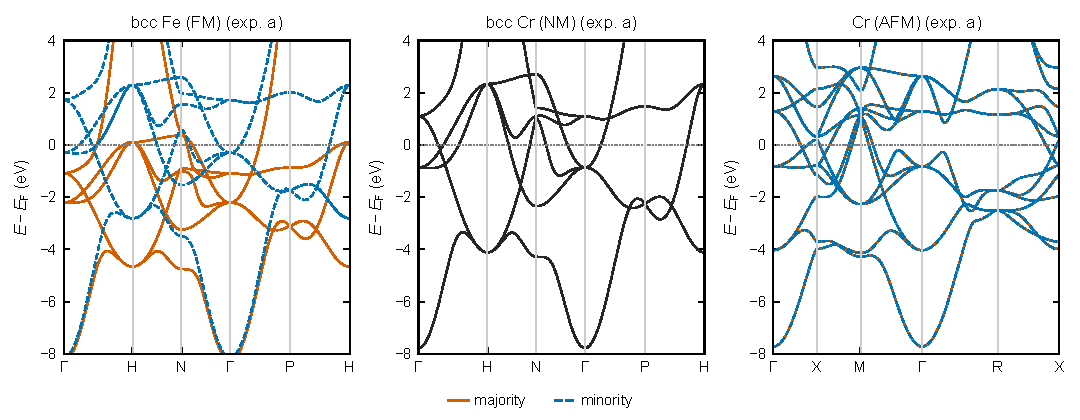
\includegraphics[width=\textwidth]{figures/kdense_scripta/supplementary/S_bands_pure_aexp_v2.pdf}
\caption{Electronic band structures of \textit{bcc} Fe (FM), \textit{bcc} Cr (NM) and AFM Cr at the room-temperature experimental lattice parameters (Fe 2.8665 \AA, Cr 2.8846 \AA), for comparison with Fig.~\ref{fig:S_bands_pure} at the relaxed PBE lattice parameters. Validation: the Fe $\Gamma$--H bands agree with EMTO-CPA \cite{korzhavyi2009electronic} to an RMS of 0.18 eV (spin up) and 0.14 eV (spin down), slightly better than at the relaxed lattice parameter.}
\label{fig:S_bands_aexp}
\end{figure}

\begin{figure}[!htbp]
\centering
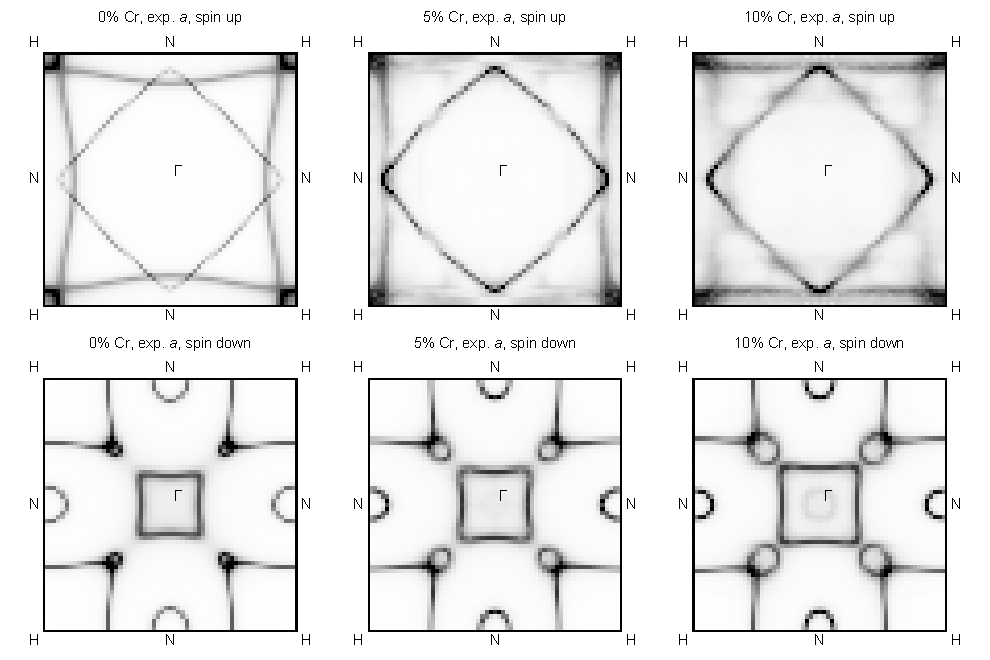
\includegraphics[width=0.76\textwidth]{figures/kdense_scripta/supplementary/S_fermi_unfolded_aexp_v2.pdf}\\[2pt]
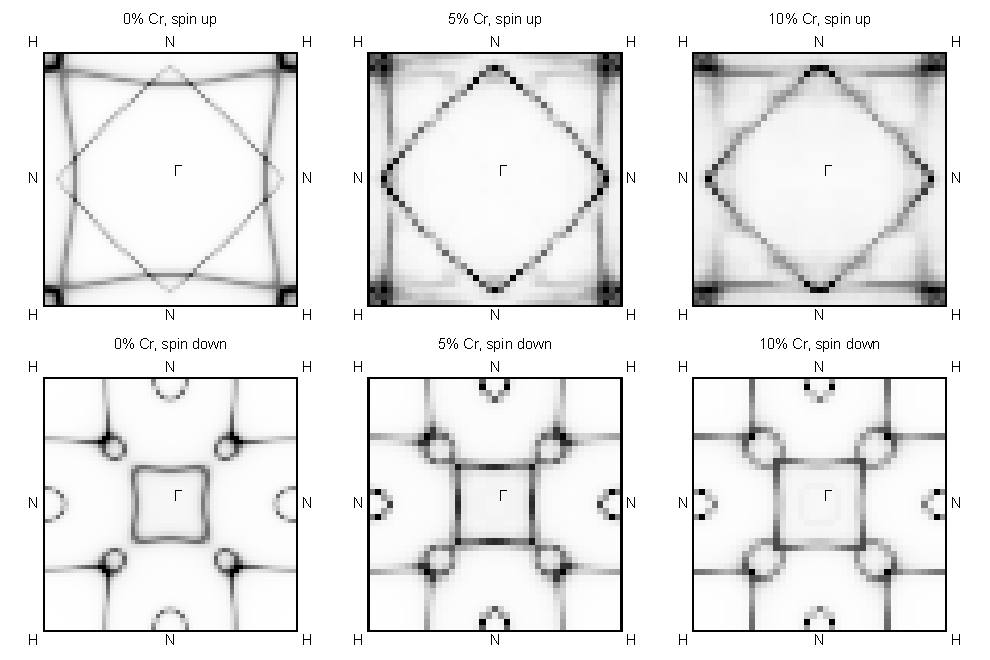
\includegraphics[width=0.76\textwidth]{figures/kdense_scripta/supplementary/S_fermi_unfolded_relaxed_v3.pdf}
\caption{Unfolded Fermi surfaces (Bloch spectral function at $E_{\mathrm F}$, $k_z=0$; spin up top, spin down bottom) of the 40-atom SQS, in the layout of Korzhavyi \textit{et al.}\ \cite{korzhavyi2009electronic} (their Fig.~6). Top: 0, 5 and 10\% Cr at the experimental lattice parameter. Bottom: 0, 5 and 10\% Cr at the PBE-relaxed lattice parameter. The supercell bands were unfolded onto the \textit{bcc} zone with BandUPpy (band step with ParO diagonalisation), on a 61$\times$61 grid except for the relaxed 5 and 10\% Cr panels (41$\times$41, hence coarser pixels). Pure Fe reproduces the Fermi surface of the primitive cell (Fig.~\ref{fig:S_fermi_Fe}) at both lattice parameters. With Cr the spin-up sheet changes topology: the arms that connect the H pockets through N lose their weight and the $\Gamma$-centred sheet reaches N. The change is already clear at 5\% Cr at both lattice parameters, and 10\% Cr looks the same with more disorder broadening, while the spin-down sheets barely change. This is the spin-up topology change that Ref.~\cite{korzhavyi2009electronic} places between 5 and 10\% Cr, the electronic origin of the Fe-rich elastic anomaly (Fig.~\ref{fig:S_fe_rich}); in our SQS it sets in slightly earlier, consistent with the critical level of Fig.~\ref{fig:S_ett}a reaching $E_{\mathrm F}$ at 5\% Cr.}
\label{fig:S_fermi_unfolded}
\end{figure}

\begin{figure}[!htbp]
\centering
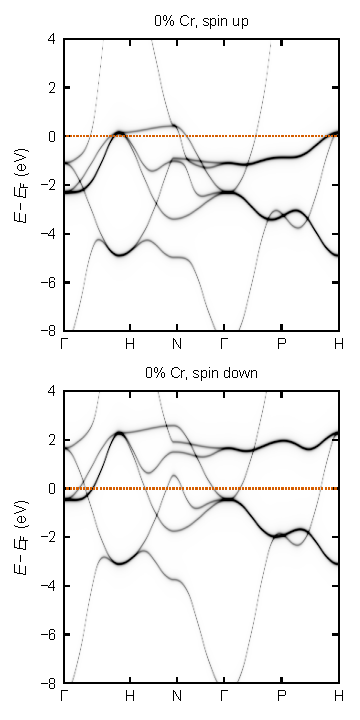
\includegraphics[width=0.36\textwidth]{figures/kdense_scripta/supplementary/S_bands_unfolded.pdf}
\caption{Unfolded (effective) band structure of the 40-atom SQS of pure Fe along $\Gamma$--H--N--$\Gamma$--P--H, spin up (top) and down (bottom), Lorentzian-broadened by 0.06 eV. It reproduces the primitive-cell bands (Fig.~\ref{fig:S_bands_pure}), including the majority H level 0.15 eV above $E_{\mathrm F}$, which validates the unfolding before it is applied to the alloys (Fig.~\ref{fig:S_bands_unfolded_aexp}).}
\label{fig:S_bands_unfolded}
\end{figure}

\begin{figure}[!htbp]
\centering
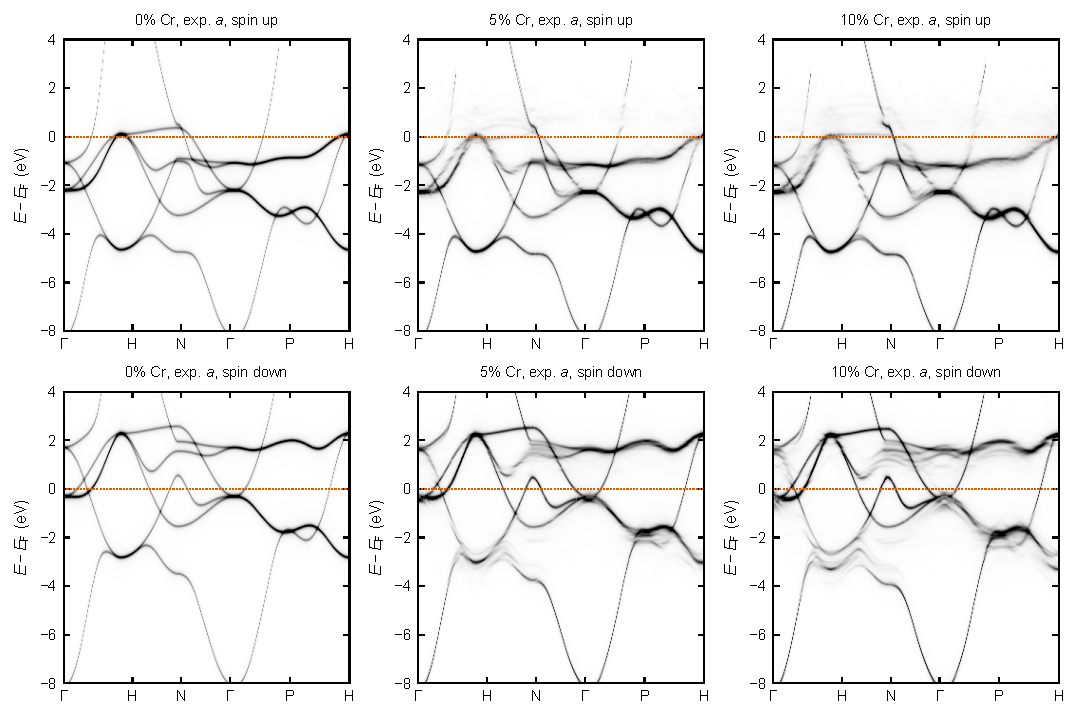
\includegraphics[width=0.9\textwidth]{figures/kdense_scripta/supplementary/S_bands_unfolded_aexp_v2.pdf}
\caption{Unfolded band structures of the 40-atom SQS at 0, 5 and 10\% Cr at the experimental lattice parameter, spin up (top) and down (bottom), as in Fig.~\ref{fig:S_bands_unfolded}. The 0\% Cr cell reproduces the primitive-cell bands of Fig.~\ref{fig:S_bands_aexp}. Cr broadens the bands (disorder) and moves the majority level at H from 0.104 eV above $E_{\mathrm F}$ (0\%) to 0.005 eV above (5\%) and 0.009 eV below (10\%), with a disorder spread of about 0.1 eV; these are the points of Fig.~\ref{fig:S_ett}a.}
\label{fig:S_bands_unfolded_aexp}
\end{figure}

\begin{figure}[!htbp]
\centering
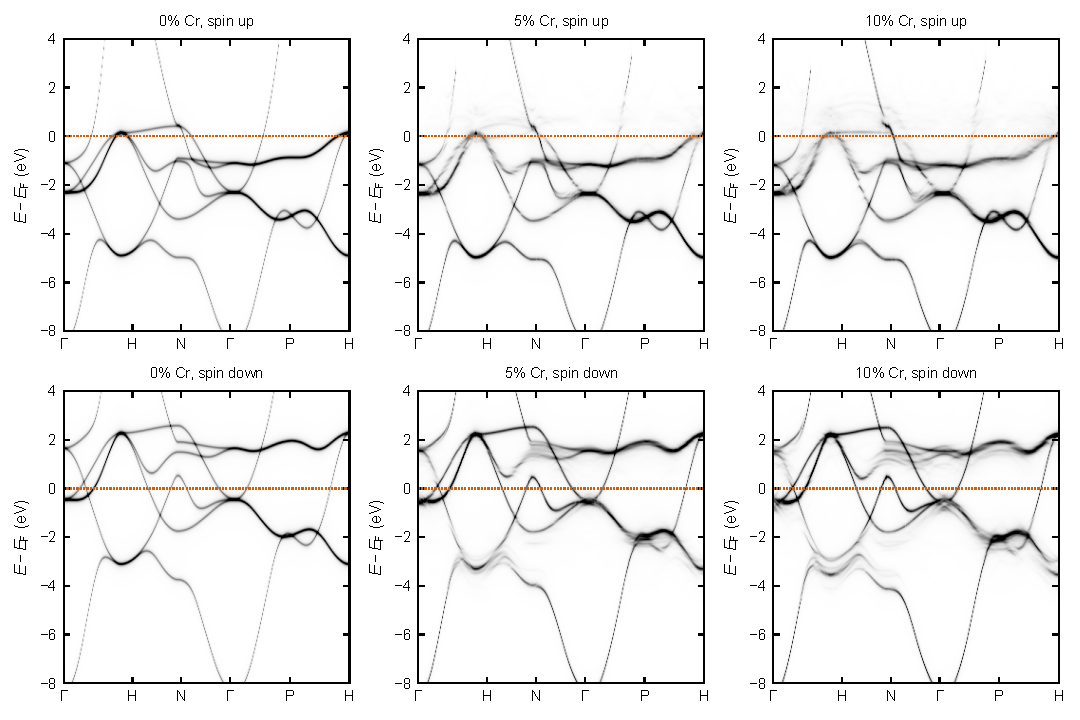
\includegraphics[width=0.9\textwidth]{figures/kdense_scripta/supplementary/S_bands_unfolded_relaxed.pdf}
\caption{Unfolded band structures of the 40-atom SQS at 0, 5 and 10\% Cr at the PBE-relaxed lattice parameter, spin up (top) and down (bottom), as in Fig.~\ref{fig:S_bands_unfolded_aexp}. The majority level at H lies 0.149 eV above $E_{\mathrm F}$ at 0\%~Cr and 0.065 and 0.068 eV above it at 5 and 10\%~Cr, with disorder spreads of 0.12 and 0.11 eV; these are the relaxed-lattice points of Fig.~\ref{fig:S_ett}a.}
\label{fig:S_bands_unfolded_relaxed}
\end{figure}

\begin{figure}[!htbp]
\centering
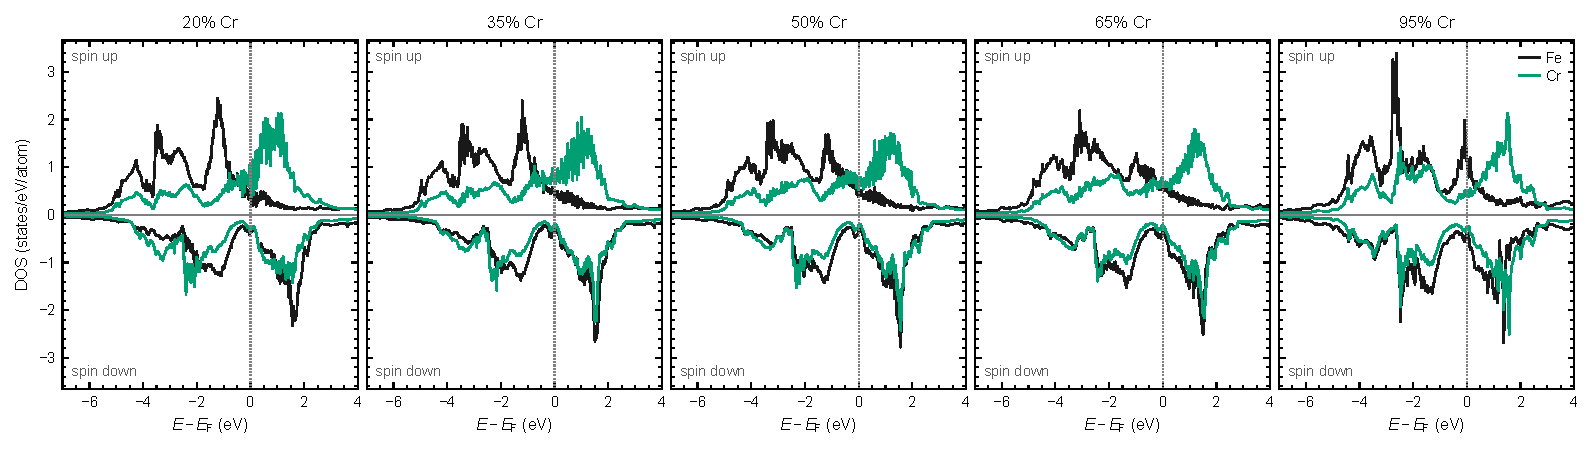
\includegraphics[width=\textwidth]{figures/kdense_scripta/supplementary/S_dos_sqs_wide_v2.pdf}
\caption{Fe- and Cr-projected densities of states per atom of the relaxed 40-atom SQS (spin up above, spin down below the axis), in the layout of Korzhavyi \textit{et al.}\ \cite{korzhavyi2009electronic} (their Fig.~4). Validation: the Fermi-level DOS, 0.79--0.98 states/eV/atom at 20--95\% Cr, lies 9--21\% below the EMTO-CPA ferromagnetic values of Ref.~\cite{korzhavyi2009electronic} (their Fig.~3d) and follows the same composition trend; the average site moments agree with EMTO-CPA (their Fig.~8) to 0.08 $\mu_{\mathrm B}$ for Fe and 0.07 $\mu_{\mathrm B}$ for Cr, and lie within the spread of VASP supercell values of Klaver \textit{et al.}\ \cite{klaver2006magnetism}. The energy window extends to 4 eV above $E_{\mathrm F}$ (1.6 times the occupied bands).}
\label{fig:S_dos}
\end{figure}
\FloatBarrier
\clearpage
\subsection*{S6. Electronic topological transition and the Fe-rich elastic anomaly}
The Fe-rich anomaly of the elastic constants (Fig.~\ref{fig:S_fe_rich}) coincides with a change of the spin-up Fermi-surface topology (Fig.~\ref{fig:S_fermi_unfolded}; Ref.~\cite{korzhavyi2009electronic}). It can be described quantitatively as an electronic topological transition (ETT) in the sense of Lifshitz \cite{lifshitz1960anomalies,varlamov1989kinetic}. Let $E_c$ be the energy of the critical point, here the triply degenerate majority-spin level at H, and $z=E_{\mathrm F}-E_c$. When $z$ changes sign, the electronic grand potential acquires a non-analytic term,
\begin{equation}
\delta\Omega(z) = -c_L\,|z|^{5/2}\,\theta(z), \qquad \delta N(E_{\mathrm F}) \propto z^{1/2}\theta(z),
\label{eq:ett_omega}
\end{equation}
so that the singular part of an elastic constant, a second strain derivative of the energy, is
\begin{equation}
\delta C_{ij} = \frac{\partial^2 \delta\Omega}{\partial\varepsilon_i\,\partial\varepsilon_j} \simeq -\tfrac{15}{4}\,c_L\,\frac{\partial z}{\partial\varepsilon_i}\frac{\partial z}{\partial\varepsilon_j}\, z^{1/2}\,\theta(z) + O\!\left(z^{3/2}\right).
\label{eq:ett_c}
\end{equation}
This is the band term $C_{\rm band}\propto-\sum_k(\partial\varepsilon_k/\partial\eta)^2\delta(\varepsilon_k-E_{\mathrm F})$ of the new Fermi-surface sheet. Alloying shifts the critical level approximately linearly, $z\simeq\kappa(x-x_c)$, and substitutional disorder broadens it. Every modulus and the SAW frequency therefore follow
\begin{equation}
Q(x) = a + b\,x + A\left[\mathrm{Re}\sqrt{x-x_c+i\Gamma}-\mathrm{Re}\sqrt{-x_c+i\Gamma}\right],
\label{eq:ett_fit}
\end{equation}
a smooth background plus a square-root anomaly whose onset $x_c$ and width $\Gamma$ are common to all quantities; $a$, $b$ and $A$ differ between them. The sign of $A$ depends on the modulus, because at fixed electron number the shift of $E_{\mathrm F}$ also enters. The test of this description is whether one onset, fixed independently by the electronic structure, accounts for every data set (Fig.~\ref{fig:S_ett}).

\textit{Onset from our electronic structure.} In ferromagnetic Fe the critical level lies $0.149$ eV above $E_{\mathrm F}$ at the PBE-relaxed lattice parameter and $0.104$ eV above it at the experimental one, so $\partial z/\partial\ln V\simeq1.07$ eV. In the unfolded bands of the SQS at the experimental lattice parameter (Fig.~\ref{fig:S_bands_unfolded_aexp}), the weight of this level at H is centred $0.005$ eV above $E_{\mathrm F}$ at 5\%~Cr ($z=-0.005$ eV) and $0.009$ eV below it at 10\%~Cr ($z=+0.009$ eV), with disorder spreads of $0.11$ and $0.10$ eV. A straight line through the three experimental-lattice points gives $\kappa=1.13$ eV and $x_c=0.079$, with the spread corresponding to $\pm0.10$ in composition (Fig.~\ref{fig:S_ett}a). The level reaches $E_{\mathrm F}$ already at 5\%~Cr, so the onset may lie nearer 0.05--0.07 than the linear estimate. At the PBE-relaxed lattice parameter (Fig.~\ref{fig:S_bands_unfolded_relaxed}) the level lies 0.065 and 0.068 eV above $E_{\mathrm F}$ at 5 and 10\%~Cr and approaches it more slowly. A straight line through the three relaxed-lattice points gives $\kappa=0.81$ eV and $x_c=0.17$ ($\pm0.15$), an extrapolation beyond the composition range of the bands. The experimental-lattice estimate is the one compared with the measured moduli below.

\textit{Onset from the elastic constants.} A joint fit of Eq.~(\ref{eq:ett_fit}) to the EMTO-CPA $C_{44}$, $B$, $C'$ and $f_{\mathrm{SAW}}$ of Ref.~\cite{razumovskiy2011first} ($0\le x\le0.2$), with one shared $x_c$ and $\Gamma$, gives $x_c=0.102$ (0.093--0.108 at $\Delta\chi^2\le1$) and $\Gamma=0.056$. The RMS residuals are 1.2, 2.9 and 0.19 GPa and 1.8 MHz (Fig.~\ref{fig:S_ett}b--e). Fixing $x_c$ and $\Gamma$ to the electronic-structure values instead fits all four quantities nearly as well: RMS 1.2, 3.3 and 0.19 GPa and 1.5 MHz, $\Delta\chi^2=3.1$ (within two standard deviations of the best fit). The model-independent markers fall in the same window: the knee of the EMTO-CPA $C_{44}$ at $x=0.059$, the minimum of the EMTO-CPA bulk modulus at 0.109, and the minimum of the \emph{measured} room-temperature bulk modulus at 0.068 \cite{korzhavyi2009electronic}. A secondary minimum of the profile near $x_c\approx0.02$ ($\Delta\chi^2=1.7$), driven by the initial rise of $C_{44}$, is disfavoured. Our QE $C_{44}$ and $f_{\mathrm{SAW}}$ show the same rise and flattening between 0 and 10\%~Cr (Fig.~\ref{fig:S_ett}b,d). Only the onset is tested. The amplitudes $A$ are not interpreted, because over this window the background and the singular term are not uniquely separable.

\textit{Link to the stiffening on decomposition.} The Fe-rich $\alpha$ phase of decomposed Fe--36Cr ($x_\alpha=0.12$ in MD, 0.14 by CALPHAD at 748~K \cite{xiong2011improved}) lies beyond $x_c$ in the experimental-lattice and elastic-constant estimates (0.08--0.10), though not in the relaxed-lattice extrapolation (0.17), so decomposition carries the Fe-rich phase across the transition. Splitting the lever-rule gain of Fe--36Cr into the two phases (CALPHAD compositions) gives $+7.8\%$ for the electronic EMTO-CPA $f_{\mathrm{SAW}}(x)$, of which $\alpha$ contributes 2.4 and $\alpha'$ 5.4 percentage points, and $+5.0\%$ for the classical MD $f_{\mathrm{SAW}}(x)$ (1.4 and 3.6 points; Fig.~\ref{fig:S_ett}f). With the MD phase compositions the totals are $+7.7\%$ and $+4.0\%$, the $\alpha$ terms 2.0 and 1.4 points. The Fe-rich side, where the ETT sits, thus accounts for about 1.0 (0.6) of the 2.8 (3.7) percentage points by which the electronic stiffening exceeds the classical one; the remainder comes from the Cr-rich side. The ETT is therefore a measurable but secondary contributor to the stiffening that TGS detects.

\begin{figure}[!htbp]
\centering
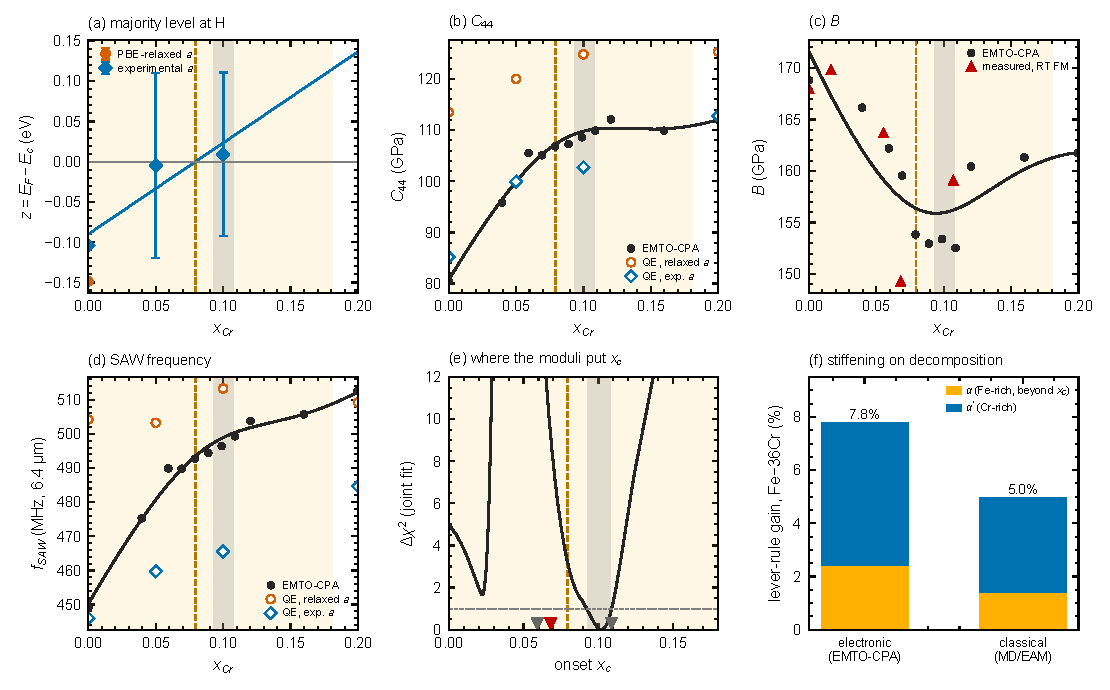
\includegraphics[width=\textwidth]{figures/kdense_scripta/supplementary/S_ett.pdf}
\caption{Electronic topological transition on the Fe-rich side. (a) Critical level $z=E_{\mathrm F}-E_c$ (majority level at H) from our band structures: pure Fe at both lattice parameters and the unfolded 5 and 10\%~Cr SQS at the experimental lattice parameter (error bars: disorder spread of the spectral weight). The line through the experimental-lattice points gives $x_c=0.079$ (dashed; light band: $\pm$ spread). (b--d) $C_{44}$, $B$ and $f_{\mathrm{SAW}}$: EMTO-CPA \cite{razumovskiy2011first} (black) with the joint fit of Eq.~(\ref{eq:ett_fit}), measured bulk moduli (red triangles, \cite{korzhavyi2009electronic}) and our QE SQS (open symbols). The grey band is the joint-fit range of $x_c$. (e) $\Delta\chi^2$ of the joint fit against the onset $x_c$; triangles mark the model-independent anomaly positions (red: measured). (f) Lever-rule stiffening of Fe--36Cr (CALPHAD phase compositions at 748~K), split into the Fe-rich $\alpha$ and Cr-rich $\alpha'$ terms, for the electronic and classical $f_{\mathrm{SAW}}(x)$. Script: \texttt{dft\_qe/ett\_analysis.py}.}
\label{fig:S_ett}
\end{figure}
\FloatBarrier
\clearpage
\subsection*{S7. Lattice dynamics}
Phonon dispersions of Fe, non-magnetic Cr and antiferromagnetic Cr are shown in Fig.~\ref{fig:S_phonons}, the $k$-point convergence that removes spurious imaginary modes of non-magnetic Cr in Fig.~\ref{fig:S_phonon_conv}, and the comparison with neutron and nuclear inelastic scattering in Fig.~\ref{fig:S_phonons_exp}. Cr is computed with density-functional perturbation theory; Fe by finite displacements, for the reason given in the captions.

\begin{figure}[!htbp]
\centering
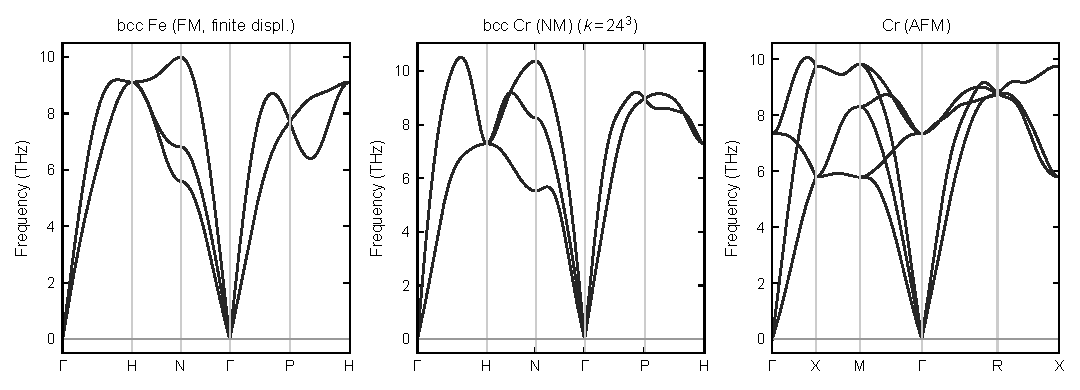
\includegraphics[width=\textwidth]{figures/kdense_scripta/supplementary/S_phonons_v2.pdf}
\caption{Phonon dispersions of \textit{bcc} Fe (FM), \textit{bcc} Cr (NM, DFPT, $k=24^3$) and commensurate AFM Cr (DFPT, $k=12^3$, simple-cubic path), at the PBE-relaxed lattice parameters. All frequencies are real. Fe phonons are computed by finite displacements (phonopy; 0.01 \AA\ displacement in a cubic $3\times3\times3$ conventional supercell of 54 atoms, same PBE-PAW settings, $k=5^3$), because density-functional perturbation theory (QE \texttt{ph.x}) gave frequencies about 60\% too high for ferromagnetic Fe while a frozen phonon with identical settings agreed with neutron scattering to 2\% (4.40 vs 4.31 THz for the transverse mode at $\zeta=1/3$ along $\Gamma$--H). A $2\times2\times5$ supercell was not used: its tetragonal shape made the symmetrised force constants inconsistent and produced a spurious imaginary branch. Cr is computed with DFPT, which agrees with neutron scattering (Fig.~\ref{fig:S_phonons_exp}); its non-magnetic phase needs $k=24^3$ (Fig.~\ref{fig:S_phonon_conv}).}
\label{fig:S_phonons}
\end{figure}

\begin{figure}[!htbp]
\centering
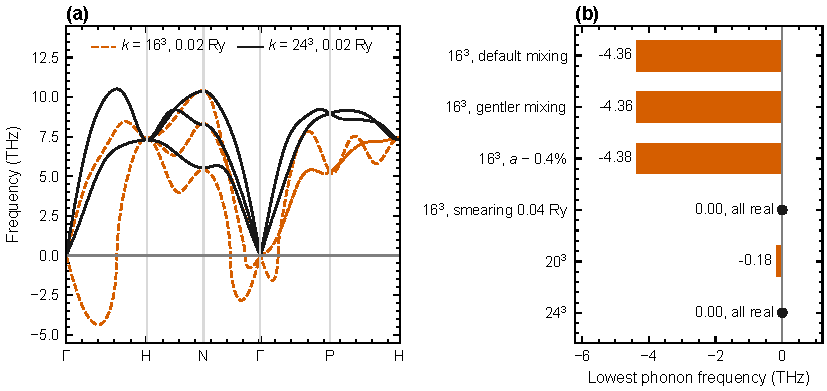
\includegraphics[width=0.85\textwidth]{figures/kdense_scripta/response/R_phonon_convergence.pdf}
\caption{Brillouin-zone sampling of the NM Cr phonons. (a) Dispersion at an electronic $k$-mesh of $16^3$ (imaginary branches plotted below zero) and $24^3$ (all real). (b) Lowest frequency along the path for each setting: SCF mixing and a 0.4\% change of the lattice parameter have no effect, whereas a denser mesh or wider smearing removes the imaginary modes. They are an artefact of under-sampling the nested Fermi surface of Cr, not a dynamical instability.}
\label{fig:S_phonon_conv}
\end{figure}

\begin{figure}[!htbp]
\centering
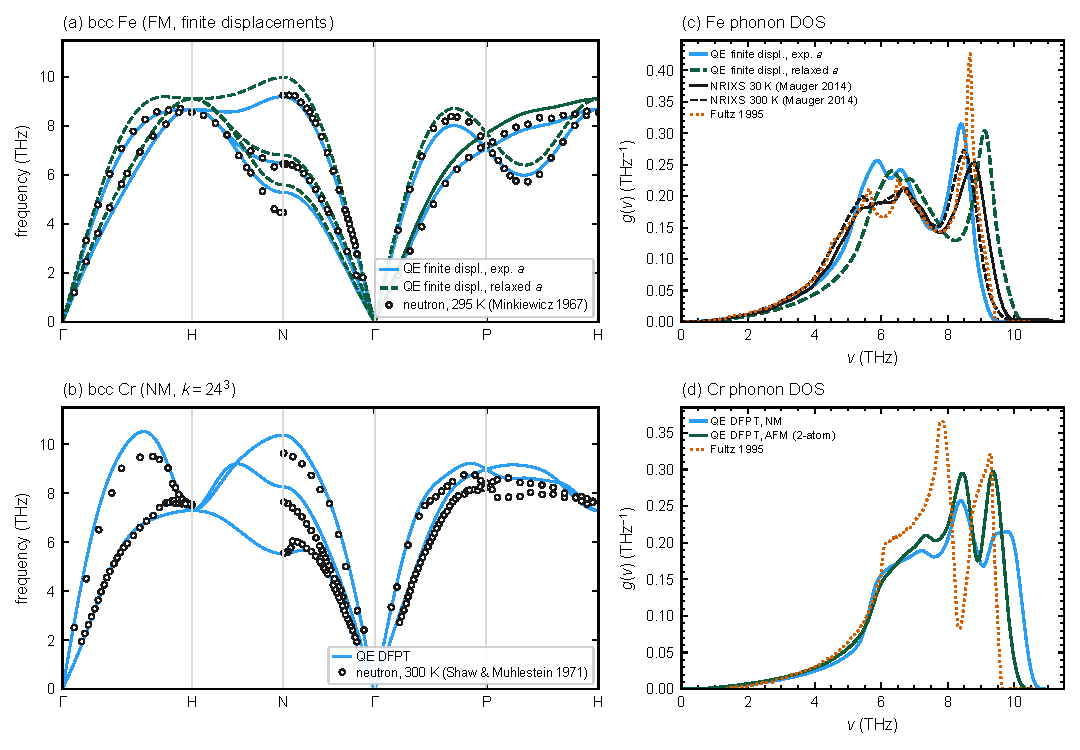
\includegraphics[width=\textwidth]{figures/kdense_scripta/supplementary/S_phonons_vs_exp_v2.pdf}
\caption{Our phonons against experiment. (a) Fe by finite displacements at the experimental (solid) and PBE-relaxed (dashed) lattice parameter, with the room-temperature neutron dispersion of Minkiewicz \textit{et al.}\ \cite{minkiewicz1967phonon}; (b) non-magnetic Cr (DFPT, $k=24^3$) with the 300 K neutron data of Shaw and Muhlestein \cite{shaw1971investigation}; (c) Fe phonon DOS against nuclear inelastic scattering at 30 and 300 K (Mauger \textit{et al.}\ \cite{mauger2014nonharmonic}) and the force-constant DOS of Fultz \textit{et al.}\ \cite{fultz1995phonon}; (d) Cr phonon DOS (NM and AFM) against Fultz \textit{et al.} Agreement (nearest-branch RMS deviation from the neutron data; mean frequency against the reference DOS): Fe 0.23 THz and $-0.1\%$ at the experimental lattice parameter, 0.46 THz and $+7.8\%$ at the relaxed one; Cr 0.41 THz (NM) and 0.35 THz (AFM), $+6\%$ and $+3\%$. Fe phonons are computed by finite displacements (phonopy; 0.01 \AA\ displacement in a cubic $3\times3\times3$ conventional supercell of 54 atoms, same PBE-PAW settings, $k=5^3$), because density-functional perturbation theory (QE \texttt{ph.x}) gave frequencies about 60\% too high for ferromagnetic Fe while a frozen phonon with identical settings agreed with neutron scattering to 2\% (4.40 vs 4.31 THz for the transverse mode at $\zeta=1/3$ along $\Gamma$--H). A $2\times2\times5$ supercell was not used: its tetragonal shape made the symmetrised force constants inconsistent and produced a spurious imaginary branch.}
\label{fig:S_phonons_exp}
\end{figure}
\FloatBarrier
\clearpage
\subsection*{S8. Validation against literature and experiment}
Every quantity shown in Sections S4--S7 was replotted on top of published data it should reproduce (Figs.~\ref{fig:V_bulk}--\ref{fig:V_phdos_Cr}). Literature curves were digitized from the published figures (raster images; the uncertainty of each digitization is given with the data in the repository, and each was checked by overlaying it on the original figure). Deviations are summarised in Table~\ref{tab:validation}; the full list, including every composition, is in \texttt{validation\_summary.csv}.

\begin{table}[!htbp]
\centering
\caption{Validation of the first-principles calculations. RMS: root-mean-square deviation; for dispersions, the deviation of each experimental point from the nearest calculated branch. ``Relaxed'': PBE-relaxed lattice parameter; ``exp.\ $a$'': room-temperature experimental lattice parameter.}
\label{tab:validation}
\small
\begin{tabular}{@{}p{3.0cm}p{4.2cm}p{6.6cm}@{}}
\toprule
Quantity & Reference & Agreement \\
\midrule
Bulk modulus & measured, compiled in Ref.~\cite{korzhavyi2009electronic} & relaxed: $+28\%$ (QE Fe), $+31\%$ (QE, 95\% Cr), $+32\%$ (VASP Fe); exp.\ $a$: $+1\%$ (QE Fe), $-7\%$ (QE AFM Cr), $+7\%$ (QE, 95\% Cr) \\
Site moments & EMTO-CPA FM \cite{korzhavyi2009electronic}; VASP supercells \cite{klaver2006magnetism} & mean $|\Delta m|$: Fe 0.08, Cr 0.07 $\mu_{\mathrm B}$ (relaxed); Fe 0.18, Cr 0.03 $\mu_{\mathrm B}$ (exp.\ $a$); within the supercell spread \\
$N(E_{\mathrm F})$ & EMTO-CPA FM \cite{korzhavyi2009electronic} & 9--21\% lower, same composition trend \\
Fe bands, $\Gamma$--H & EMTO-CPA, pure Fe \cite{korzhavyi2009electronic} & RMS 0.22/0.17 eV (spin up/down, relaxed); 0.18/0.14 eV (exp.\ $a$) \\
Cr phonons & neutron, 300 K \cite{shaw1971investigation} & RMS 0.35--0.41 THz, bias $-0.05$ to $+0.17$ THz (NM and AFM, both lattice parameters) \\
Cr phonon DOS & force-constant DOS \cite{fultz1995phonon} & mean frequency $+6\%$ (NM), $+3\%$ (AFM); exp.\ $a$: $-0.4\%$, $+1.0\%$ \\
Fe phonons & neutron, 295 K \cite{minkiewicz1967phonon} & finite displacements: RMS 0.23 THz (exp.\ $a$), 0.46 THz (relaxed); DFPT: 1.1--1.4 THz (not used) \\
Fe phonon DOS & NRIXS, 30 and 300 K \cite{mauger2014nonharmonic} & mean frequency $-0.1\%$ (exp.\ $a$), $+7.8\%$ (relaxed); DFPT $+19$ to $+27\%$ \\
\bottomrule
\end{tabular}
\end{table}

The electronic structure and magnetism agree well with the literature, and the Cr lattice dynamics agree with neutron scattering. The bulk modulus is the important exception. At the PBE-relaxed volume both DFT codes overestimate the measured bulk modulus by about 30\%, the usual consequence of the too-small PBE volume of Fe--Cr; at the room-temperature experimental lattice parameter the QE value at 95\% Cr is within 7\% of experiment. The same setting reproduces the minimum of the bulk modulus and the plateau of $f_{\mathrm{SAW}}$ near 40\% Cr reported with EMTO-CPA at experimental lattice parameters \cite{razumovskiy2011first}, which argues for basing the QE elastic constants on the experimental-lattice-parameter series. For Fe, density-functional perturbation theory is too stiff at both lattice parameters (Figs.~\ref{fig:V_phdisp_Fe} and \ref{fig:V_phdos_Fe}), whereas finite displacements with the same pseudopotential, cutoff and $k$-point density agree with neutron and NRIXS data; the Fe phonons are therefore taken from finite displacements (Fig.~\ref{fig:S_phonons}). The pure-metal electronic DOS (Fig.~\ref{fig:S_dos_pure}) reproduces the EMTO-CPA DOS of the Fe site in Fe$_{98}$Cr$_2$ \cite{korzhavyi2009electronic}, with $N(E_{\mathrm F})$ within 0.05 states/eV per spin.

\begin{figure}[!htbp]
\centering
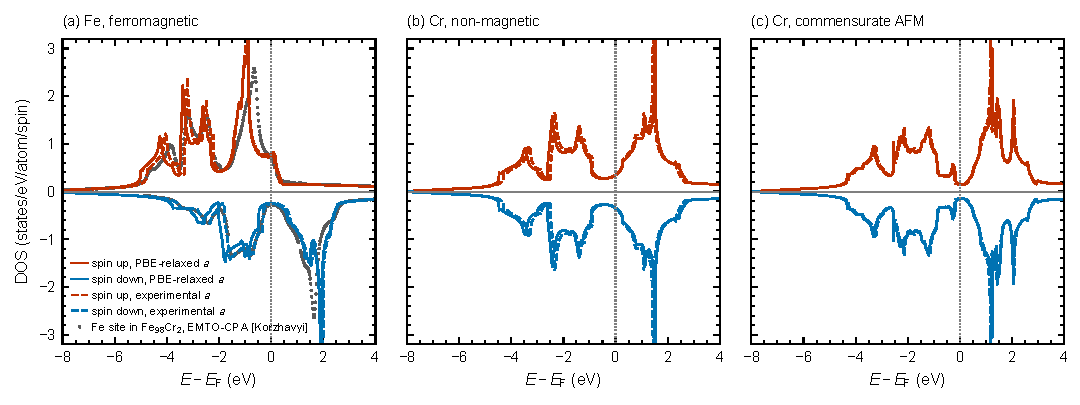
\includegraphics[width=\textwidth]{figures/kdense_scripta/supplementary/S_dos_pure.pdf}
\caption{Spin-resolved total density of states of the pure metals (QE, optimised tetrahedra, $36^3$ mesh for the \textit{bcc} cells and $24^3$ for the 2-atom AFM Cr cell) at the PBE-relaxed (solid) and experimental (dashed) lattice parameter; spin down is plotted downwards, and the two channels of non-magnetic Cr are equal. (a) Fe, with the EMTO-CPA DOS of the Fe site in Fe$_{98}$Cr$_2$ (dots, digitized from Fig.~4 of Ref.~\cite{korzhavyi2009electronic}). $N(E_{\mathrm F})$ of Fe is 0.74 (spin up) and 0.24 (spin down) states/eV against 0.69 and 0.29 there, and the main majority and minority peaks lie 0.2--0.3 eV further from $E_{\mathrm F}$ in PBE than in the LDA of Ref.~\cite{korzhavyi2009electronic}. Total $N(E_{\mathrm F})$: 0.98 (Fe), 0.68 (non-magnetic Cr) and 0.30 (AFM Cr) states/eV/atom at the PBE-relaxed lattice parameter, within 0.07 at the experimental one. With the measured electronic specific-heat coefficients (Fe 4.98, Cr 1.40 mJ\,mol$^{-1}$\,K$^{-2}$ \cite{kittel2005introduction}) these imply a mass enhancement $1+\lambda\approx2.0$--2.2 for FM Fe and AFM Cr, whereas non-magnetic Cr would require $1+\lambda<1$.}
\label{fig:S_dos_pure}
\end{figure}

\paragraph{Thermal transport (Section S1).} The estimates of Section S1 depend only on $E$, $\rho$ and the molar mass and were evaluated for every tensor of this work (Fig.~\ref{fig:S_thermal}). The elastic Debye temperature of Fe is 450~K (QE, experimental lattice parameter), 453~K (EMTO-CPA) and 472~K (MD), against 470~K from calorimetry \cite{kittel2005introduction}; for Cr, 585--605~K against 630~K. Debye temperatures from the second moment of the phonon DOS, a definition that runs lower, agree with experiment on the same definition: 415~K for our Fe against 417--431~K from NRIXS, and 466~K for our AFM Cr against 460~K from the neutron-based DOS of Fultz \textit{et al.} The minimum thermal conductivity of Eq.~(S2), $\kappa_{\min}=1.15$--1.6~W/(m\,K), gives $D_{\min}=\kappa_{\min}/\rho c_p=0.32$--$0.48\times10^{-6}$~m$^2$/s, an order of magnitude below the thermal diffusivity measured by TGS in CF8 ($3.5\times10^{-6}$~m$^2$/s, Fig.~\ref{fig5}d). This is expected, since $\kappa_{\min}$ is a lower bound on the lattice contribution and electrons carry most of the heat in a metal. The relative changes do not depend on the prefactor. On full decomposition of MD Fe--36Cr, $E$ rises by 9.5\% and the S1 scaling $D\propto E^{1/2}$ gives $\Delta D/D=+4.6\%$, close to the $+4.0\%$ measured after aging at 290~$^\circ$C. The larger increases measured after aging at 330--400~$^\circ$C ($+20$ to $+29\%$) exceed what lattice stiffening alone can produce; they point to the electronic contribution, which the S1 estimate does not include. Panels (e) and (f) of Fig.~\ref{fig5} now follow Eq.~(S2) as printed; the earlier version of the working sheet had evaluated $\kappa$ with Planck's constant ($\times10^{11}$) in place of $k_B$ and with $m=2$, which overstated $\kappa$ and $D$ by a factor of 7.6 without changing their trend.

\begin{figure}[!htbp]
\centering
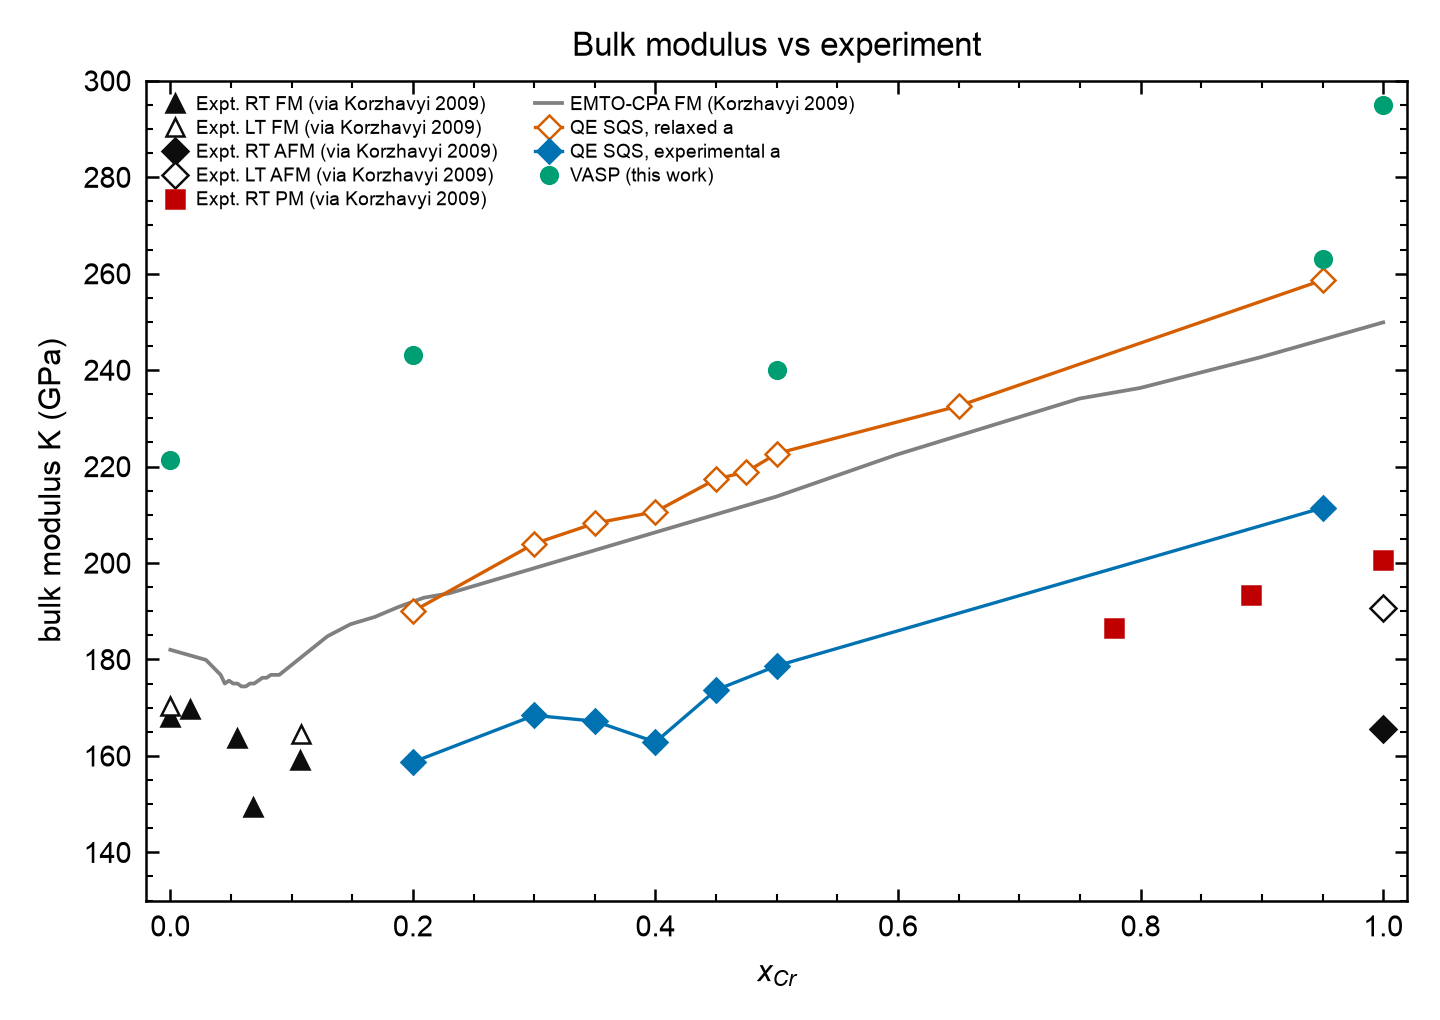
\includegraphics[width=0.85\textwidth]{figures/kdense_scripta/supplementary/validation/V_bulk_modulus.png}
\caption{Bulk modulus against experiment. Markers: measured values compiled by Korzhavyi \textit{et al.}\ \cite{korzhavyi2009electronic} (RT and LT; FM, AFM and paramagnetic); grey line: their EMTO-CPA FM calculation. QE SQS (diamonds) and pure elements (squares; 2-atom cells, $k=16^3$, Fe FM and Cr AFM) at the PBE-relaxed (open) and the room-temperature experimental (filled) lattice parameter; VASP (circles). At the relaxed volume both codes overestimate $B$: QE by $+28\%$ (Fe) and $+31\%$ (95\% Cr), VASP by $+32\%$ (Fe). At the experimental lattice parameter QE gives $B=170$ GPa for Fe ($+1\%$ against 168 GPa), $-7\%$ for AFM Cr and $+7\%$ at 95\% Cr. The experimental lattice parameter was therefore adopted for the additional QE series of Section S4; PBE underestimates the Fe--Cr volume by about 4\%, and the bulk modulus is the property most sensitive to it.}
\label{fig:V_bulk}
\end{figure}

\begin{figure}[!htbp]
\centering
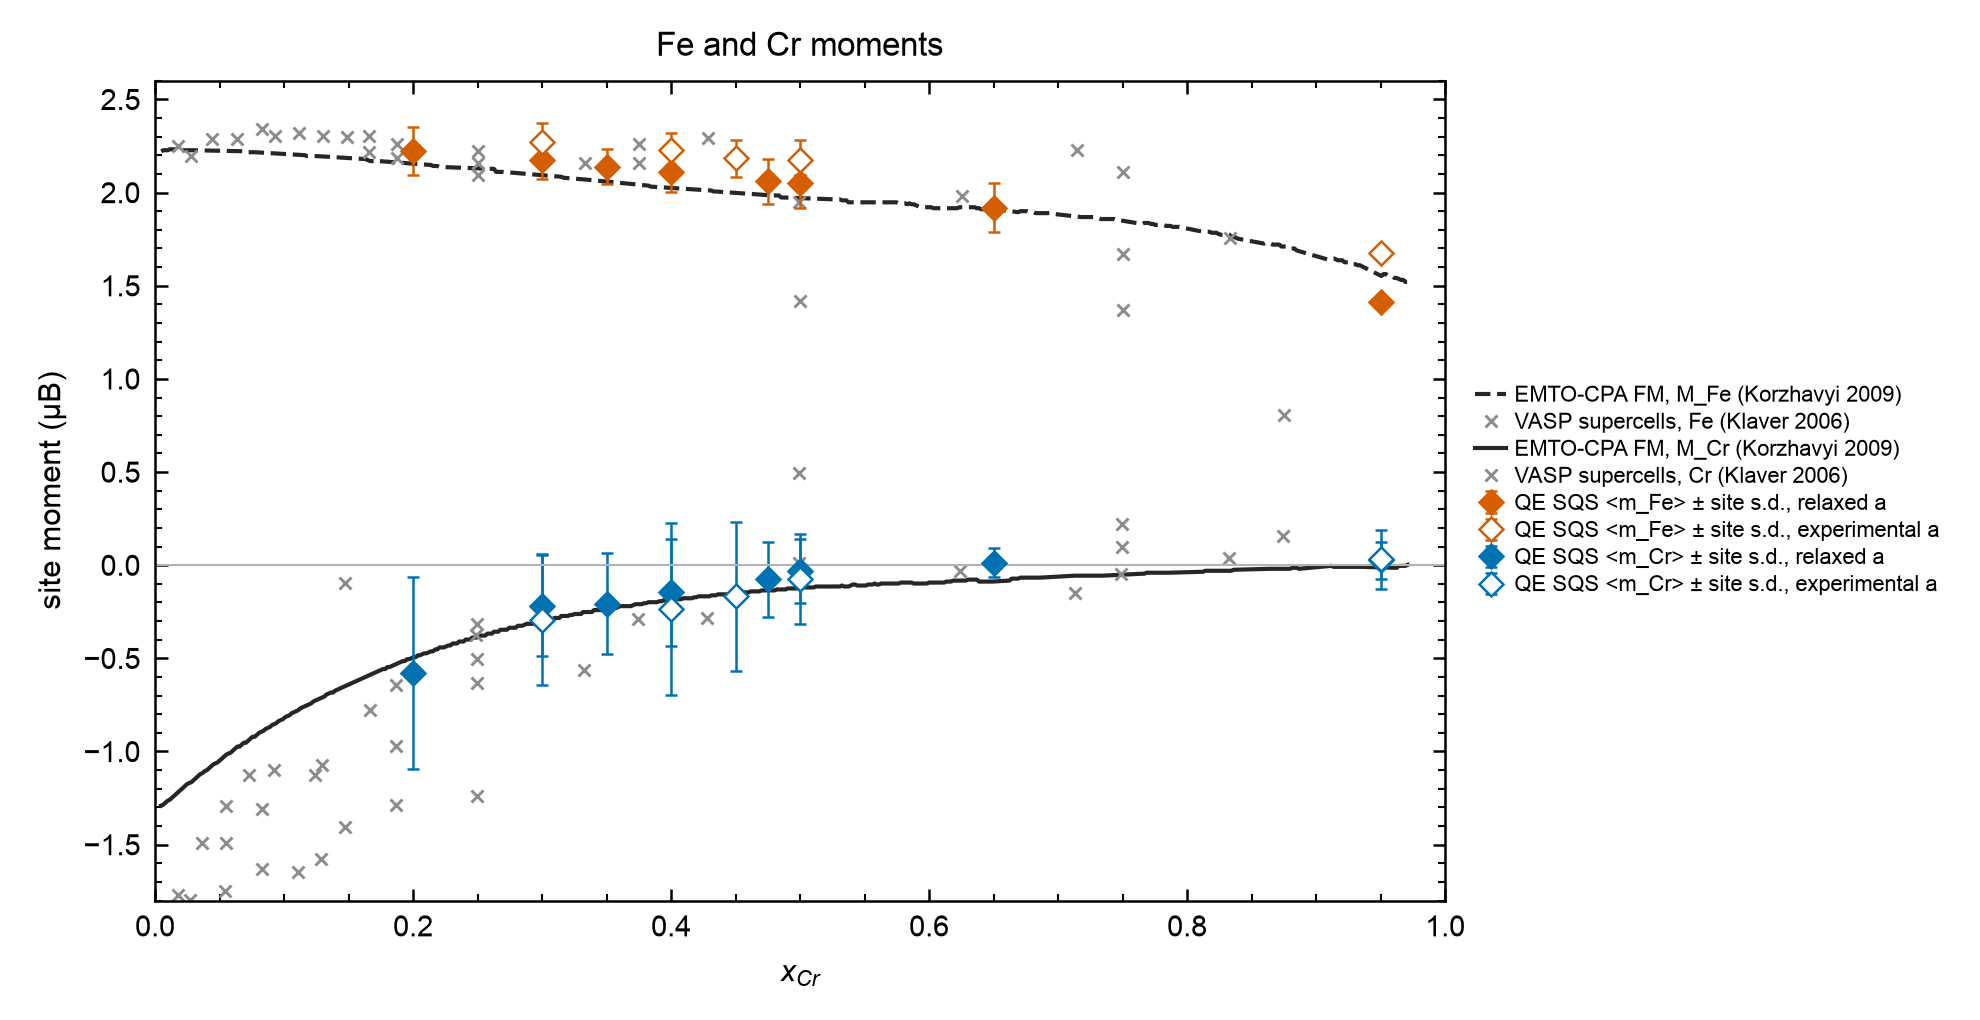
\includegraphics[width=0.85\textwidth]{figures/kdense_scripta/supplementary/validation/V_moments.png}
\caption{Average Fe and Cr site moments of the QE SQS (error bars: standard deviation over sites) at the relaxed (filled) and experimental (open) lattice parameter, against EMTO-CPA FM (lines; Korzhavyi \textit{et al.}\ \cite{korzhavyi2009electronic}, Fig.~8, $a_0=2.875$ \AA) and VASP supercells (crosses; Klaver \textit{et al.}\ \cite{klaver2006magnetism}). The collapse of the Cr moment between 20 and 50\% Cr is reproduced.}
\label{fig:V_moments}
\end{figure}

\begin{figure}[!htbp]
\centering
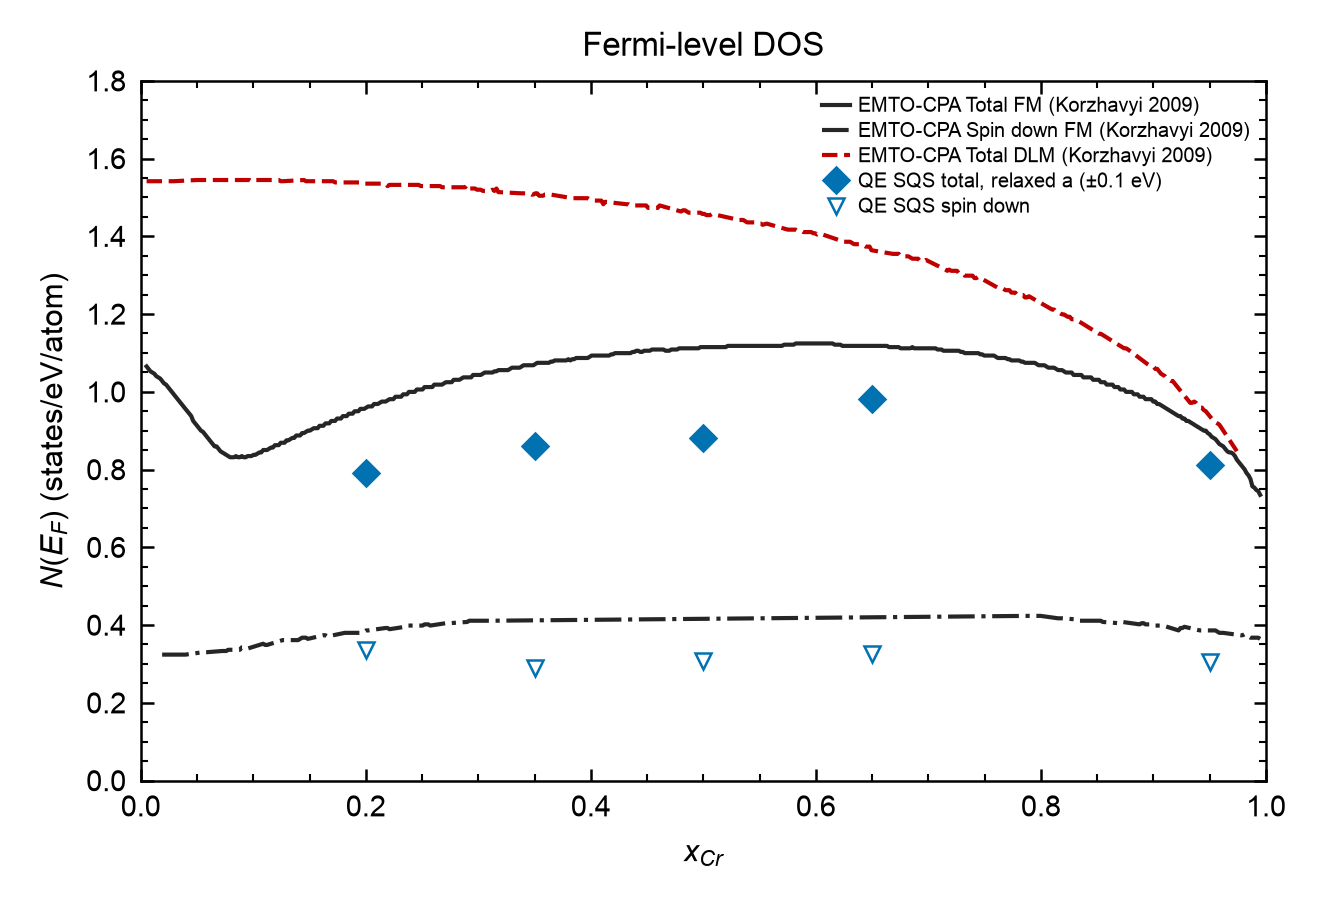
\includegraphics[width=0.7\textwidth]{figures/kdense_scripta/supplementary/validation/V_nef.png}
\caption{Fermi-level density of states per atom of the relaxed QE SQS (total and spin down, averaged over $\pm0.1$ eV) against EMTO-CPA for the FM and paramagnetic (DLM) states (Korzhavyi \textit{et al.}\ \cite{korzhavyi2009electronic}, Fig.~3d). The QE values are 9--21\% lower and follow the FM composition trend.}
\label{fig:V_nef}
\end{figure}

\begin{figure}[!htbp]
\centering
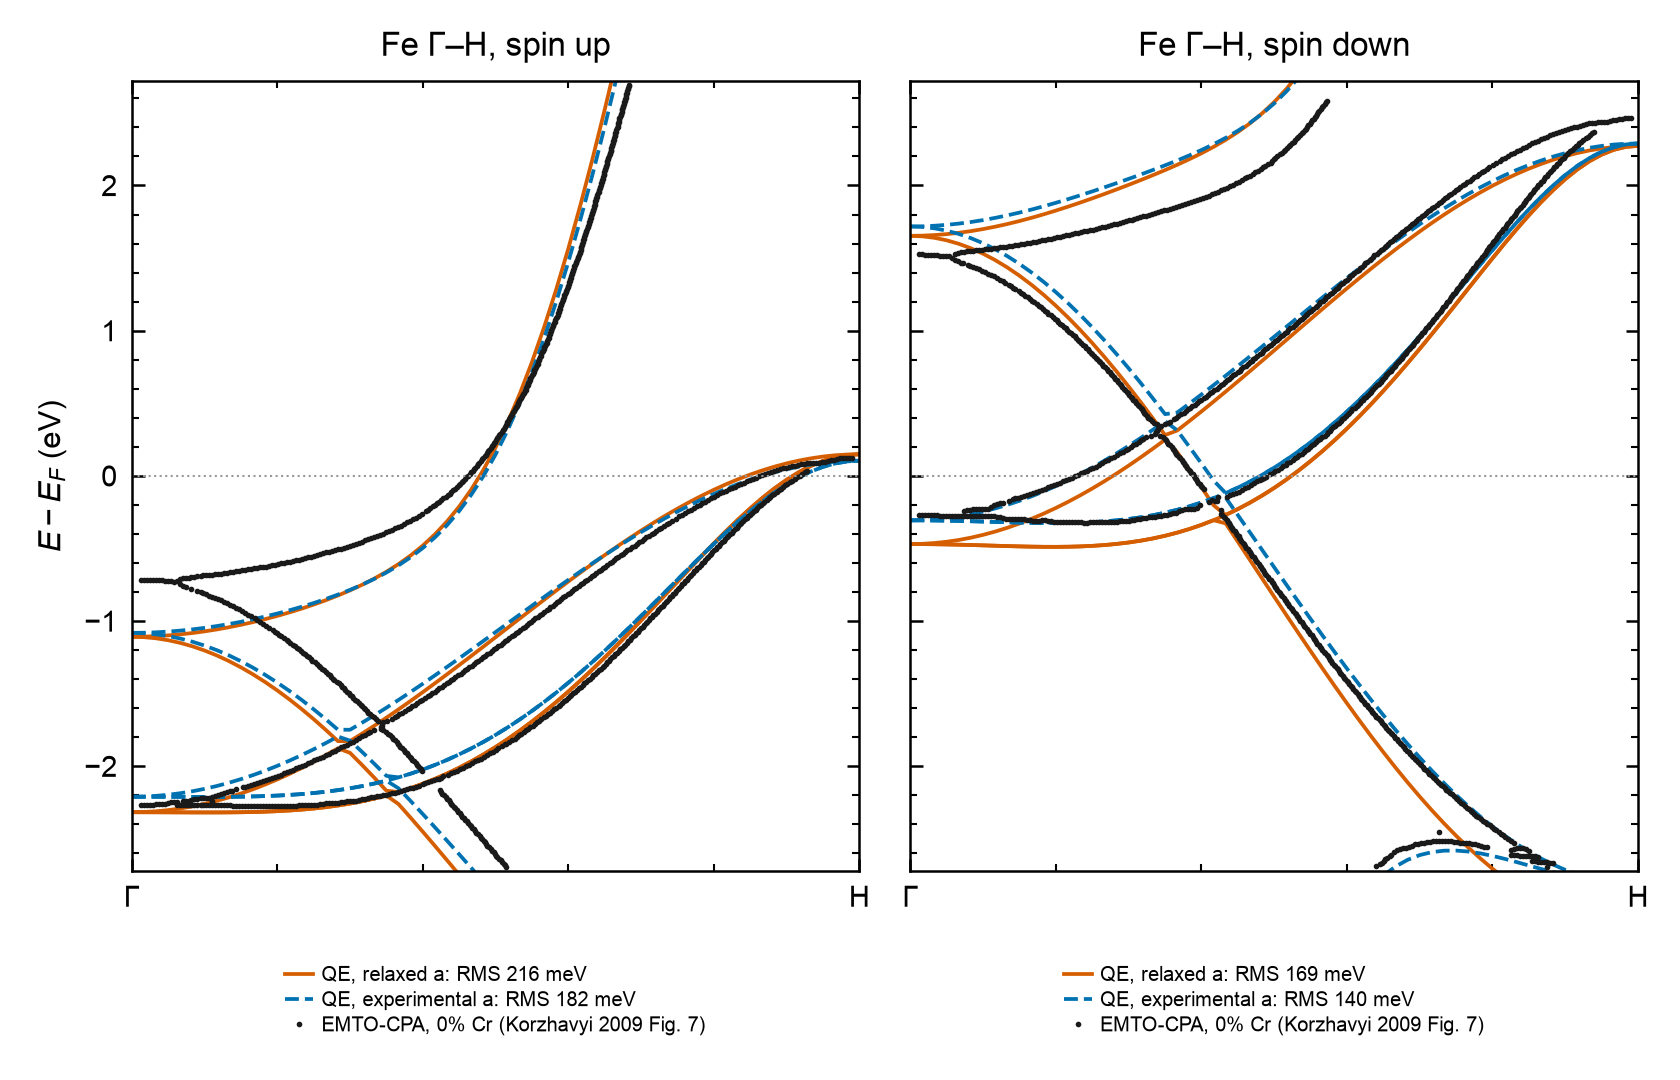
\includegraphics[width=0.85\textwidth]{figures/kdense_scripta/supplementary/validation/V_bands_Fe.png}
\caption{Band structure of FM \textit{bcc} Fe along $\Gamma$--H, majority (left) and minority (right), QE at the relaxed and experimental lattice parameters, against the EMTO-CPA spectrum of pure Fe (points; Korzhavyi \textit{et al.}\ \cite{korzhavyi2009electronic}, Fig.~7a,d; lattice parameter not stated). RMS deviations 0.14--0.22 eV; the Fermi-level crossings and the majority H level 0.15 eV above $E_{\mathrm F}$ agree.}
\label{fig:V_bands}
\end{figure}

\begin{figure}[!htbp]
\centering
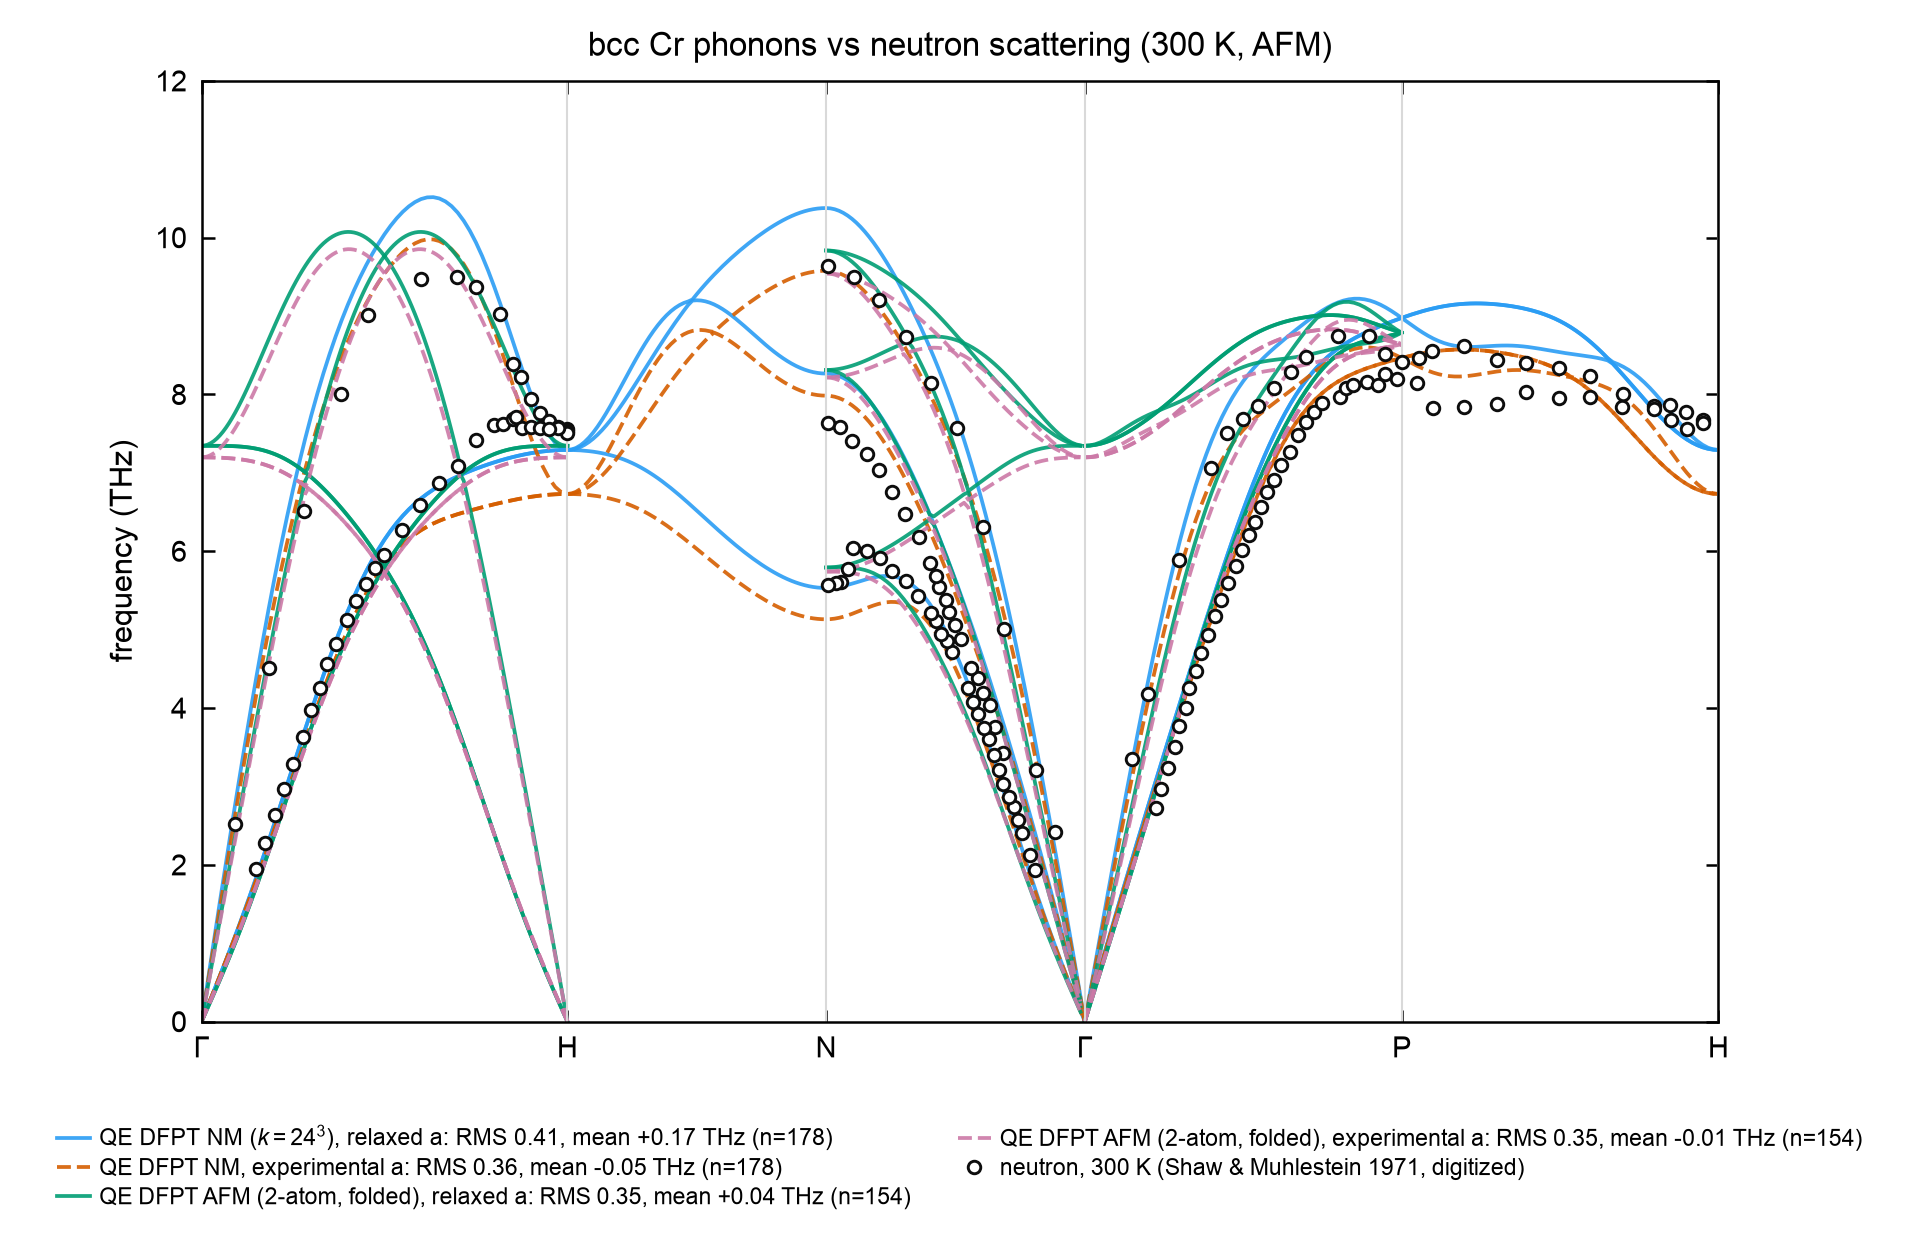
\includegraphics[width=1.0\textwidth]{figures/kdense_scripta/supplementary/validation/V_phonon_disp_Cr.png}
\caption{Phonon dispersion of Cr against neutron scattering at 300 K (Shaw and Muhlestein \cite{shaw1971investigation}, digitized; Cr is AFM at 300 K): DFPT for NM Cr ($k=24^3$) and commensurate AFM Cr (2-atom simple-cubic cell, branches folded onto the \textit{bcc} path where the lines coincide), each at the relaxed and the experimental lattice parameter. RMS deviations 0.35--0.41 THz.}
\label{fig:V_phdisp_Cr}
\end{figure}

\begin{figure}[!htbp]
\centering
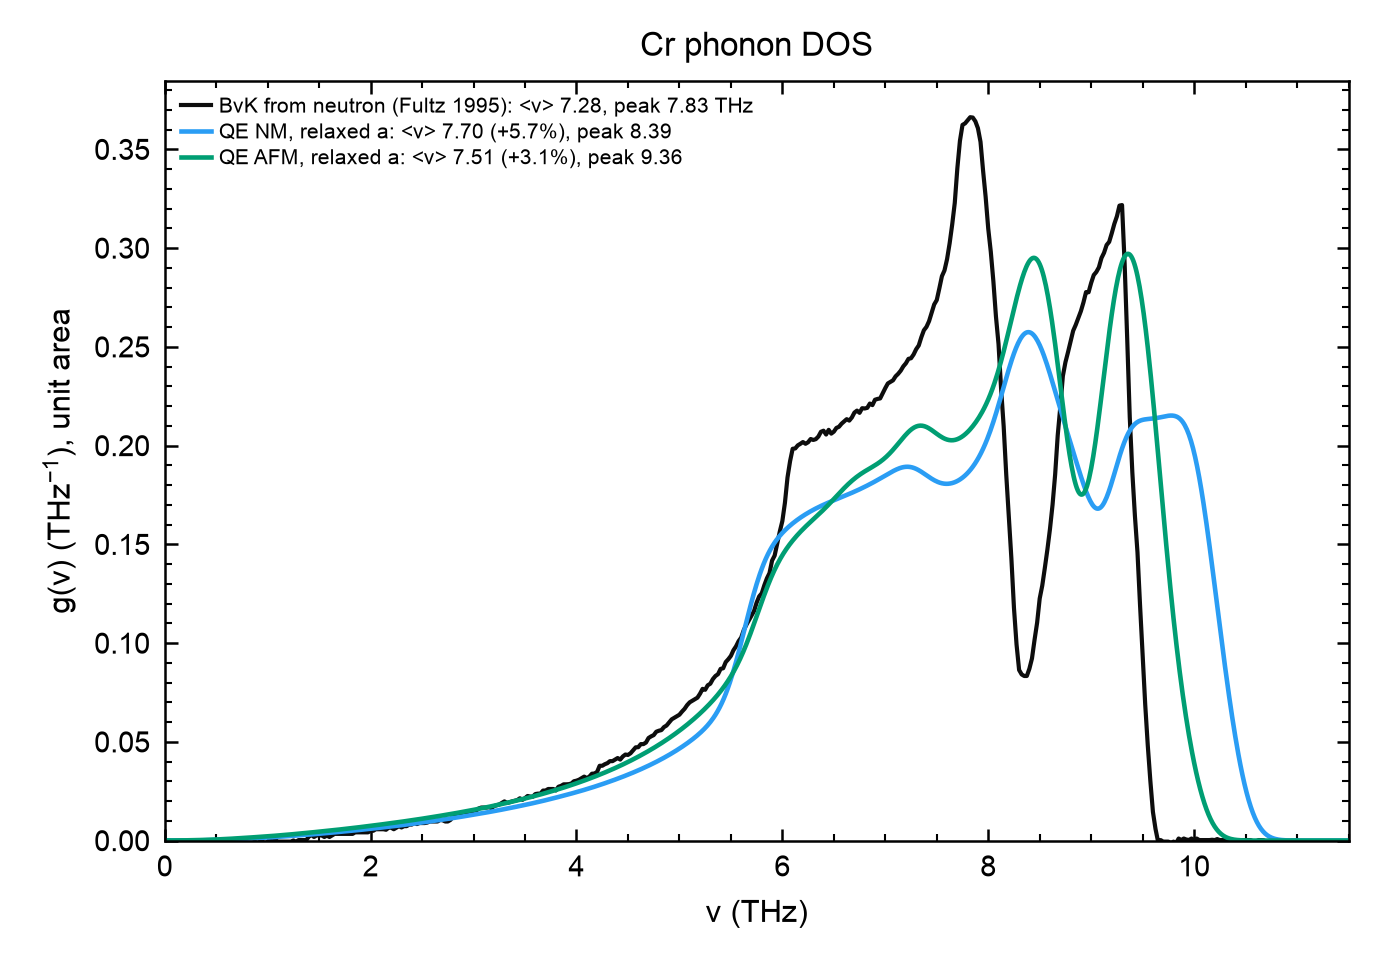
\includegraphics[width=0.7\textwidth]{figures/kdense_scripta/supplementary/validation/V_phonon_dos_Cr.png}
\caption{Phonon DOS of Cr (DFPT, NM and AFM, unit area) against the Born--von K\'arm\'an DOS of Fultz \textit{et al.}\ \cite{fultz1995phonon}, which is calculated from force constants fitted to neutron dispersions (not a measured spectrum). Mean frequencies are 6\% (NM) and 3\% (AFM) higher.}
\label{fig:V_phdos_Cr}
\end{figure}

\begin{figure}[!htbp]
\centering
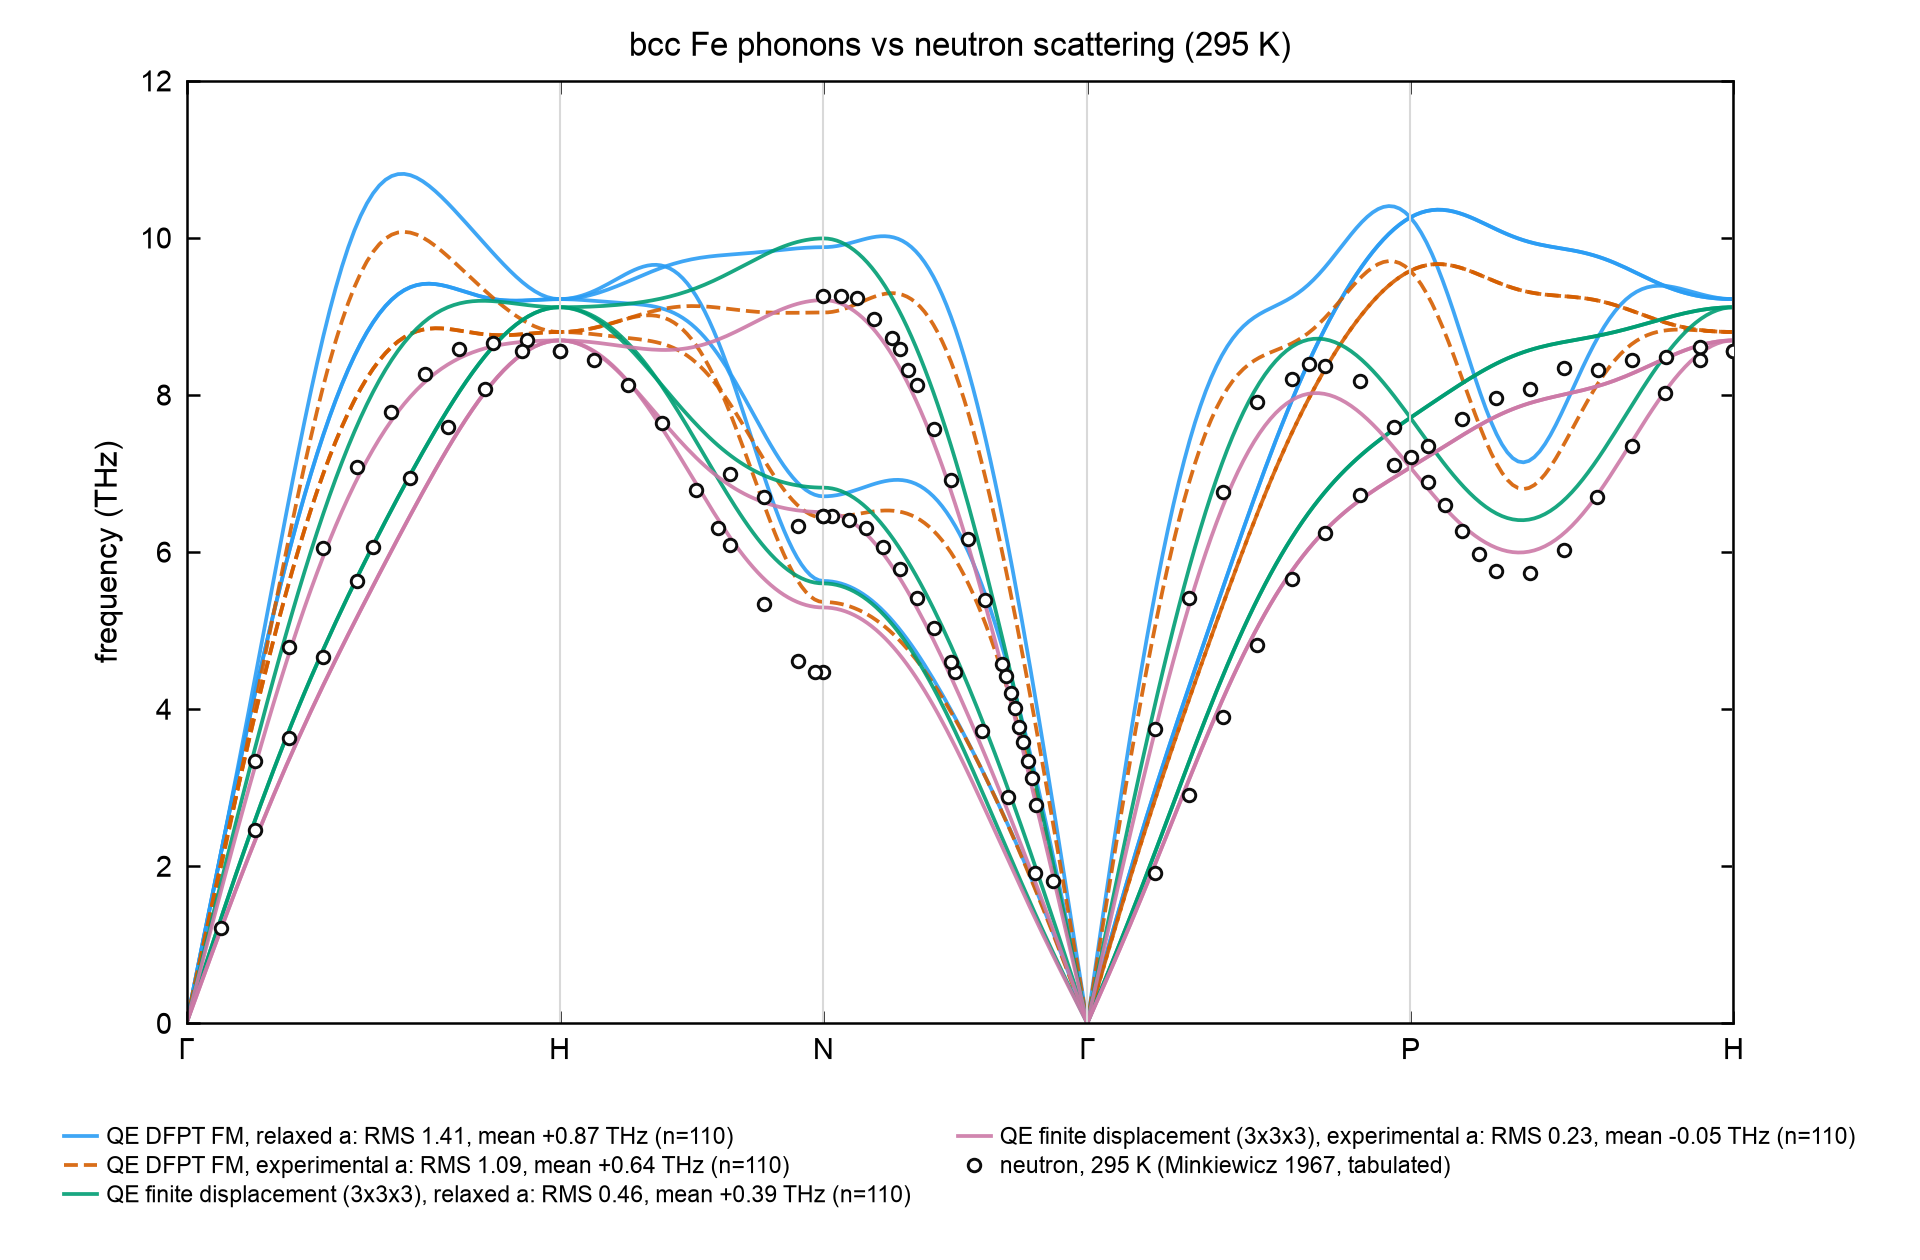
\includegraphics[width=1.0\textwidth]{figures/kdense_scripta/supplementary/validation/V_phonon_disp_Fe.png}
\caption{Phonon dispersion of FM Fe against neutron scattering at 295 K (Minkiewicz \textit{et al.}\ \cite{minkiewicz1967phonon}, tabulated): DFPT and finite displacements, each at the relaxed and the experimental lattice parameter. DFPT is too stiff (RMS 1.4 and 1.1 THz); finite displacements agree (RMS 0.46 and 0.23 THz). Fe phonons are computed by finite displacements (phonopy; 0.01 \AA\ displacement in a cubic $3\times3\times3$ conventional supercell of 54 atoms, same PBE-PAW settings, $k=5^3$), because density-functional perturbation theory (QE \texttt{ph.x}) gave frequencies about 60\% too high for ferromagnetic Fe while a frozen phonon with identical settings agreed with neutron scattering to 2\% (4.40 vs 4.31 THz for the transverse mode at $\zeta=1/3$ along $\Gamma$--H). A $2\times2\times5$ supercell was not used: its tetragonal shape made the symmetrised force constants inconsistent and produced a spurious imaginary branch.}
\label{fig:V_phdisp_Fe}
\end{figure}

\begin{figure}[!htbp]
\centering
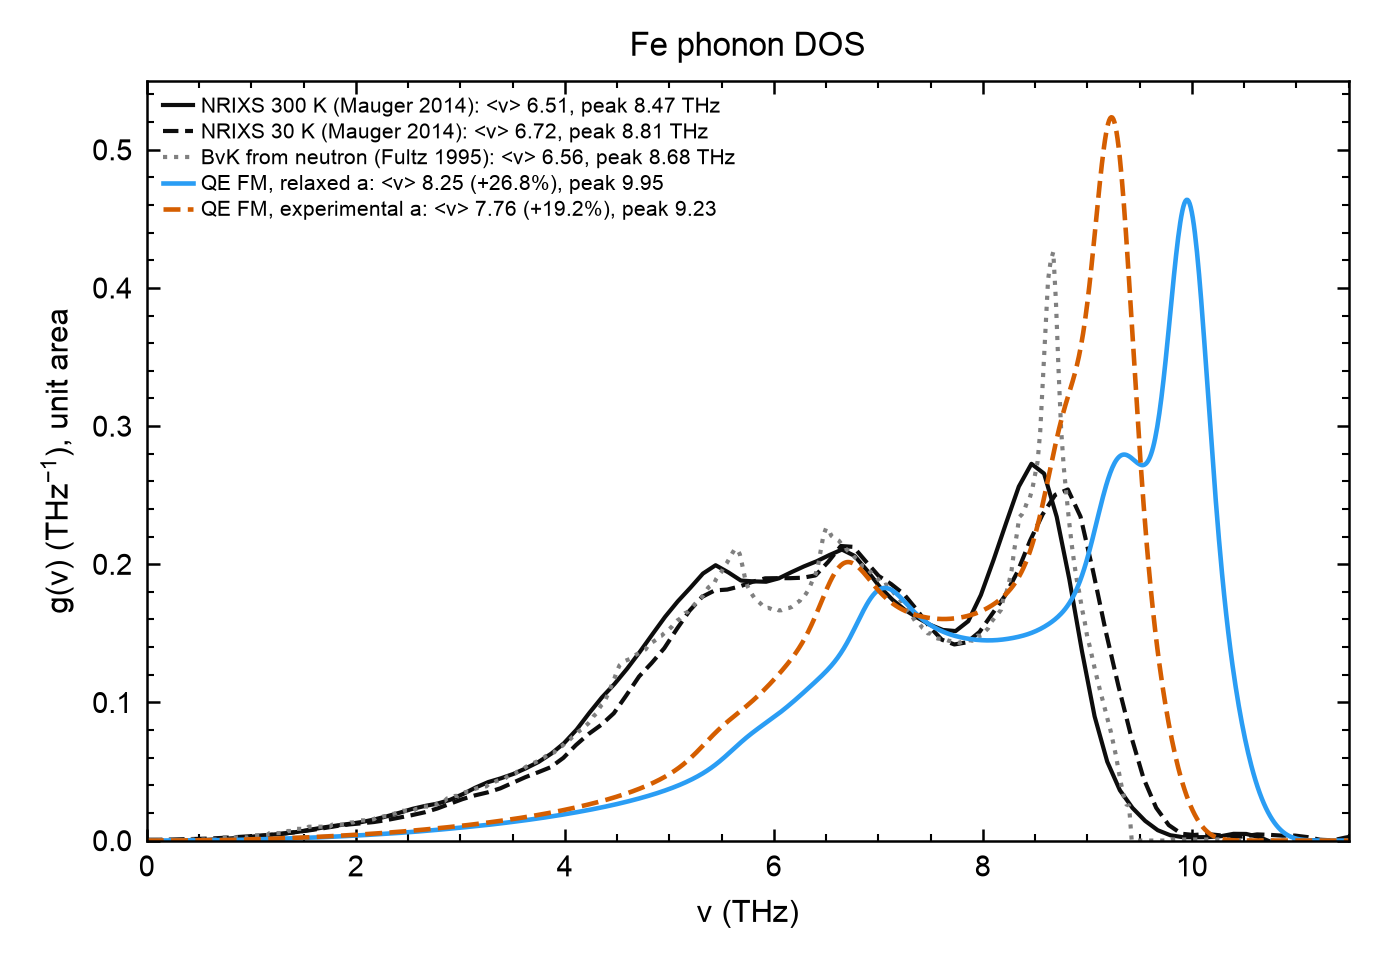
\includegraphics[width=0.7\textwidth]{figures/kdense_scripta/supplementary/validation/V_phonon_dos_Fe.png}
\caption{Phonon DOS of FM Fe (unit area) against NRIXS at 30 and 300 K (Mauger \textit{et al.}\ \cite{mauger2014nonharmonic}) and the force-constant DOS of Fultz \textit{et al.}\ \cite{fultz1995phonon}. Mean frequencies relative to the 300 K NRIXS DOS: DFPT $+27\%$ (relaxed) and $+19\%$ (experimental lattice parameter); finite displacements $+7.8\%$ and $-0.1\%$. The finite-displacement result at the experimental lattice parameter is used for Fe.}
\label{fig:V_phdos_Fe}
\end{figure}

\begin{figure}[!htbp]
\centering
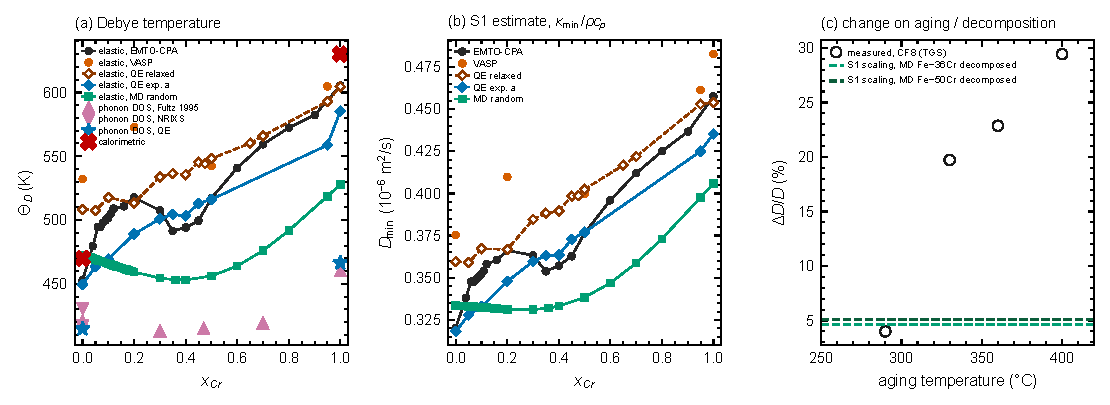
\includegraphics[width=\textwidth]{figures/kdense_scripta/supplementary/S_thermal.pdf}
\caption{Validation of the thermal-transport estimates of Section S1. (a) Debye temperature: elastic (Anderson) from every tensor of this work and EMTO-CPA; from the second moment of the phonon DOS (Fultz \textit{et al.}\ \cite{fultz1995phonon}, NRIXS \cite{mauger2014nonharmonic}, ours; this definition runs about 10\% below the elastic one); calorimetric values of Fe and Cr \cite{kittel2005introduction}. (b) $D_{\min}=\kappa_{\min}/\rho c_p$ from Eq.~(S2) of Section S1 for each tensor set; it is a lower bound on the lattice contribution. (c) Relative change of the thermal diffusivity: measured by TGS in CF8 after aging (circles, Fig.~\ref{fig5}d) and predicted by the S1 scaling for full decomposition of MD Fe--36Cr and Fe--50Cr (dashed). Script: \texttt{dft\_qe/thermal\_check.py}.}
\label{fig:S_thermal}
\end{figure}
\FloatBarrier
\subsection*{S9. Proposed mechanism figures}
The two figures below collect the mechanism behind the anomalous elasticity and the stiffening on decomposition (Fig.~\ref{fig:S_mechanism}), and its consequence for embrittlement (Fig.~\ref{fig:S_embrittlement}). They are placed here for now; we may move them to the main text.

\clearpage
\begin{figure}[!t]
\centering
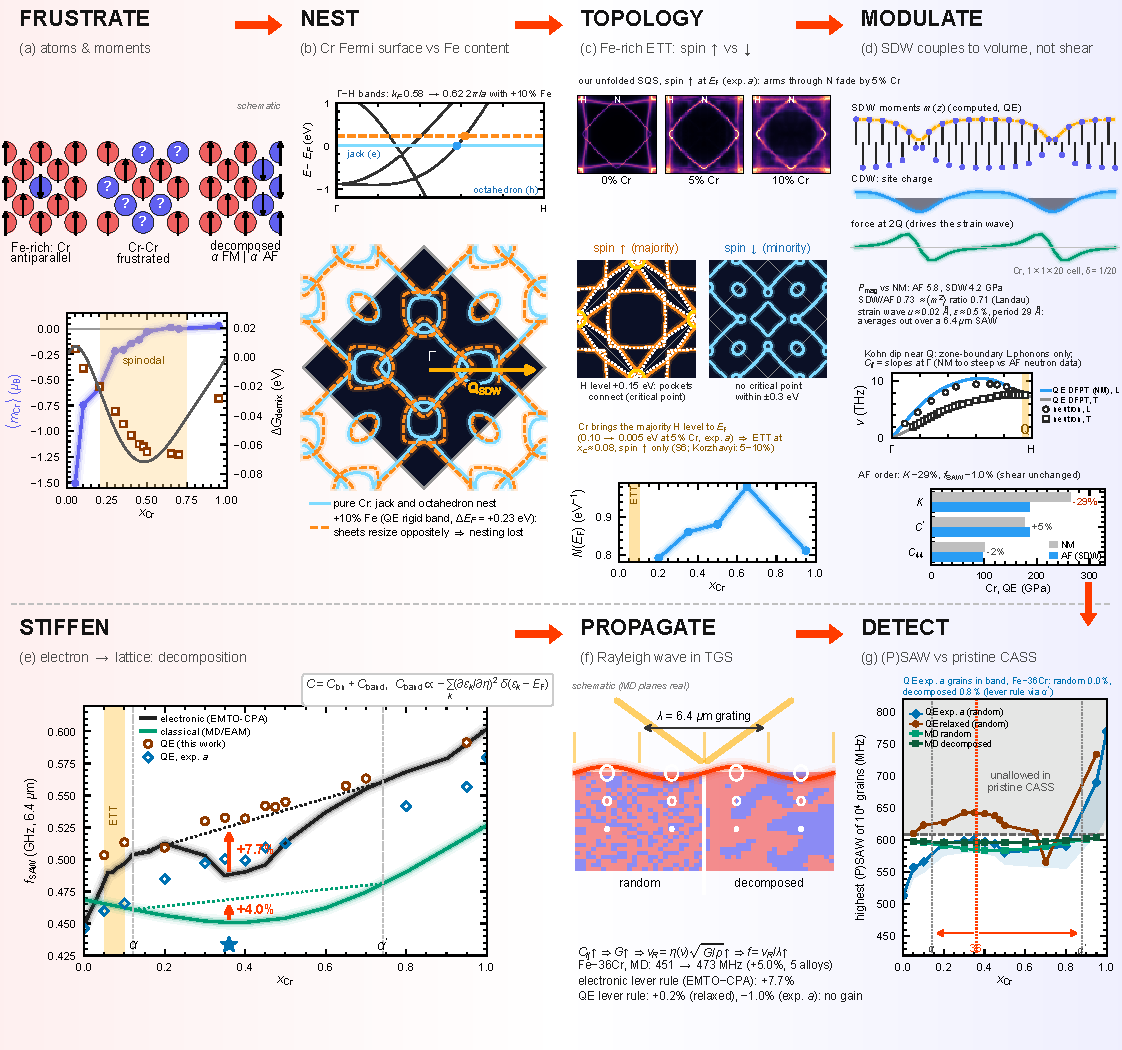
\includegraphics[width=\textwidth,height=0.80\textheight,keepaspectratio]{figures/kdense_scripta/fig4_mechanism_v11_full.pdf}
\caption{Mechanism of the anomalous elasticity of bcc Fe--Cr and of the stiffening on spinodal decomposition. Panel descriptions are on the following page.}
\label{fig:S_mechanism}
\end{figure}



\clearpage
\noindent\textbf{Figure~\ref{fig:S_mechanism} (continued).} (a) Magnetic frustration: isolated Cr is antiparallel to Fe; Cr--Cr neighbours are frustrated and the Cr moments collapse (Quantum ESPRESSO SQS, 5--95\% Cr: $\langle m_{\mathrm{Cr}}\rangle=-1.51$, $-0.75$, $-0.58$, $-0.21$, $-0.03\,\mu_{\mathrm{B}}$ at 5, 10, 20, 35, 50\% Cr), giving $\Delta G_{\mathrm{demix}}<0$ and the spinodal window (QE squares, PWSCF--PAW model line). (b) Top: non-magnetic Cr bands along $\Gamma$--H (QE); the d band that bounds the jack and the octahedron crosses $E_{\mathrm F}$ at $k_F=0.58\,(2\pi/a)$, moving to 0.62 when the same bands hold 10\% Fe (rigid band, $\Delta E_{\mathrm F}=+0.23$ eV). Bottom: Fermi surface of non-magnetic Cr (QE, $k_z=0$): the electron jack at $\Gamma$ nests onto the hole octahedron at H with $\mathbf{Q}_{\mathrm{SDW}}$; adding Fe (rigid band) resizes the two sheets in opposite senses and destroys the nesting (computed nesting function, Fig.~\ref{fig:S_nesting}) (Fe makes the SDW of Cr commensurate at about 2.3 at.\% and lowers $T_{\mathrm N}$ by 15--20 K per at.\% \cite{fawcett1988spin}). (c) Fe-rich side, by spin: Fermi-surface sections of ferromagnetic Fe (QE). In the majority channel a band level at H lies 0.15 eV above $E_{\mathrm F}$, where the H pockets connect (dotted contour, circles): this is the critical point of the electronic topological transition that Korzhavyi \textit{et al.} find in the spin-up Fermi surface at 5--10\% Cr \cite{korzhavyi2009electronic} (with the bulk-modulus anomaly of Ref.~\cite{olsson2003abinitio}). The minority channel has no critical point within $\pm0.3$ eV. Rigid filling would move $E_{\mathrm F}$ down, away from the critical level, so the transition is driven by the Cr-induced shift of the majority states rather than by band filling. Top: our unfolded SQS Fermi surfaces (spin up, experimental lattice parameter, 0, 5 and 10\% Cr; Fig.~\ref{fig:S_fermi_unfolded}). The arms through N fade by 5\% Cr, where the majority H level has reached $E_{\mathrm F}$ (0.104 eV above it in Fe, 0.005 eV at 5\% Cr), giving $x_c\approx0.08$ (Section S6). (d) In pure Cr the SDW, with its charge-density and strain waves at $2\mathbf{Q}$ \cite{fawcett1988spin}, here computed in our Cr supercell (moments, site-charge CDW and the force at $2\mathbf{Q}$; Fig.~\ref{fig:S_sdw}), leaves two lattice signatures, and neither is the stiffening. Magnetism couples to the volume: the magnetic pressure relative to the non-magnetic cell (AF 5.8, SDW 4.2 GPa) scales with $\langle m^2\rangle$ (ratio 0.73 against 0.71), and the strain wave it drives ($u\approx0.02$ \AA, $\varepsilon\approx0.5\%$, period 29 \AA) averages out over the 6.4 $\mu$m SAW wavelength. The nesting softens the longitudinal phonons near $\mathbf{Q}$ (Kohn dip; DFPT for non-magnetic Cr at $k=24^3$, and neutron scattering at 300 K \cite{shaw1971investigation}), but only near the zone boundary; the elastic constants are the slopes at $\Gamma$. Antiferromagnetic order softens the volume channel, not shear (QE, pure Cr): $C_{12}$ falls from 146 to 63 GPa and $K$ from 264 to 186 GPa ($-29\%$), while $C'$ (177 $\to$ 185 GPa) and $C_{44}$ (100 $\to$ 98 GPa) barely change, so $f_{\mathrm{SAW}}$ falls by only 1.0\%. Fe brings $T_{\mathrm N}$ below room temperature at about 1 at.\% Fe and suppresses antiferromagnetism near 18 at.\% Fe \cite{xiong2011improved}, so the Cr-rich $\alpha'$ of decomposed Fe--36Cr ($x\approx0.74$ in MD, 0.88 by CALPHAD at 748 K) is paramagnetic when TGS measures it. The stiffening on decomposition is a shear effect (e; Fig.~\ref{fig:S_embrittlement}). (e) Decomposition places the Fe-rich $\alpha$ ($x=0.12$) and Cr-rich $\alpha'$ ($x=0.74$) phases of MD Fe--36Cr on stiffer parts of a convex $f_{\mathrm{SAW}}(x)$: the lever rule gives $+4.0\%$ with the MD (classical) curve, which accounts for most of the $+5.0\%$ obtained for the fully decomposed MD structure, and $+7.7\%$ with the EMTO-CPA (electronic) curve whose random-alloy minimum lies near Fe--36Cr. With the CALPHAD phase compositions at 748 K ($\alpha$ 0.14, $\alpha'$ 0.88 \cite{xiong2011improved}) these become $+5.0\%$ (MD, matching the $+5.0\%$ of the decomposed MD structure) and $+7.8\%$ (EMTO-CPA). Neither QE curve gives a lever-rule gain ($+0.2\%$ at the PBE-relaxed and $-1.0\%$ at the experimental lattice parameter, MD phase compositions; the latter has a plateau near 35\% Cr but no minimum), so the electronic $+7.7\%$ rests on the EMTO-CPA curve. (f) Schematic of the TGS measurement over the MD microstructures (random and decomposed, real (001) planes). (g) Highest (P)SAW frequency over $10^4$ grains ($\lambda=6.4\,\mu$m) against composition, the quantity compared with the band, for the random solid solution (QE 40-atom SQS at the experimental and at the PBE-relaxed lattice parameter; MD $25^3$ cell, $\phi=0.5$) and the decomposed MD cell ($\phi=1$); shading, 95th to 100th percentile of the QE set at the experimental lattice parameter. Arrows: decomposition of Fe--36Cr into $\alpha$ (0.14) and $\alpha'$ (0.88; CALPHAD, 748~K). At the experimental lattice parameter, where the QE moduli agree with experiment, no random alloy between 0 and 80\% Cr reaches the band; the Cr-rich end does (5\% of grains at 95\% Cr, 13\% for pure Cr). Decomposed Fe--36Cr therefore has about 0.8\% of its grains in the band by the lever rule, all from the $\alpha'$ phase, against none for the random alloy. The PBE-relaxed tensors, with their too-stiff bulk moduli, reach the band at most compositions; the MD tensors never do. Full distributions as violins: Fig.~\ref{fig:S_saw_landscape}.
\clearpage

\begin{figure}[!htbp]
\centering
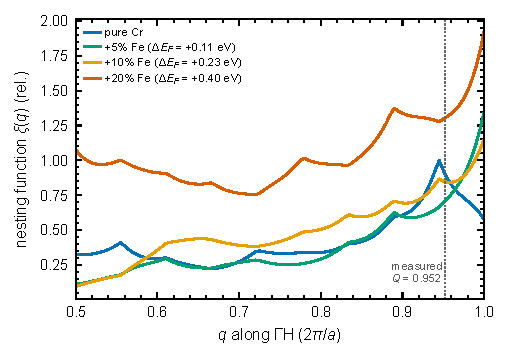
\includegraphics[width=0.6\textwidth]{figures/kdense_scripta/supplementary/S_nesting.pdf}
\caption{Nesting function $\xi(\mathbf q)=N^{-1}\sum_{\mathbf k,n,m}\delta(\varepsilon_{n\mathbf k}-E_{\mathrm F})\,\delta(\varepsilon_{m,\mathbf k+\mathbf q}-E_{\mathrm F})$ of non-magnetic \textit{bcc} Cr along $\Gamma$--H (QE bands on the full $36^3$ grid, unfolded from the irreducible wedge with the 48 operations of $O_h$; Gaussian width 0.05 eV), normalised to its pure-Cr maximum, for pure Cr and with 5, 10 and 20\% Fe added as a rigid-band filling (2 electrons per Fe). Pure Cr peaks at $q=0.945\,(2\pi/a)$, against the measured SDW wavevector $Q=0.952$ ($\delta=0.048$ at low temperature \cite{fawcett1988spin}). With Fe the incommensurate peak disappears and the maximum moves to the commensurate $q=1$ (H) by 5\% Fe, consistent with the measured incommensurate-to-commensurate transition of the SDW at about 2.3 at.\% Fe \cite{fawcett1988spin}.}
\label{fig:S_nesting}
\end{figure}



\clearpage
\textit{Why decomposed ferrite reaches the unallowed range.} Three checks constrain the mechanism stated in Sec.~3.2. (i) For any coherent arrangement of the $\alpha$ and $\alpha'$ phases the effective tensor is bounded above by their Voigt average \cite{hill1952elastic}, and the per-grain surface-wave speed rises with stiffness, so no microstructure can exceed the Voigt result. Laminate homogenization along $\langle100\rangle$ \cite{backus1962long} and full-field FFT homogenization \cite{moulinec1998numerical} reproduce the explicit MD decomposed tensors to 3--5~MHz (73--84\% of the frequency shift); for Fe--36Cr every scheme gives a highest per-grain (P)SAW of 562--582~MHz with the QE and EMTO-CPA phase tensors, below 609~MHz. Coherency stresses (0.39\% misfit, through third-order elastic constants) and the magnetic state of $\alpha'$ change this by less than 10~MHz. (ii) The top of the (P)SAW branch follows $C_{44}$ ($f\propto C_{44}^{1/2}$), which varies little across Fe--Cr (80--115~GPa) and on decomposition. (iii) Above 665~MHz, the highest frequency of any surface mode of the pristine 304 tensor at any intensity, the surface modes are weak high-velocity pseudo-SAWs (relative intensity $10^{-5}$--$10^{-3}$); the 609~MHz edge of the band corresponds to an intensity cut of at least $10^{-3}$. Across all 70 tensors of this work (QE, EMTO-CPA and MD; random and decomposed), the fraction of grains with such modes follows $C'$ (rank correlation $+0.94$) and the Zener anisotropy ($-0.95$), not $C_{44}$ ($-0.31$). Decomposition raises the effective $C'$ of Fe--36Cr by 17\% (QE) to 29\% (EMTO-CPA), and the fraction from 0.4 to 1.9\% (QE) and from 2.6 to 6.2\% (EMTO-CPA; FFT homogenization); MD, whose phases are both strongly anisotropic, gives 0.01 to 0.05\%. In the measured histogram of Ref.~\cite{al2023detecting} (Fig.~9), 0.2\% of the peaks lie above 665~MHz for unaged CASS and 2.0, 7.1, 8.1 and 14.6\% after aging at 290, 330, 360 and 400~$^\circ$C (digitized, $\pm$1--2 counts per bin). The modes are weak and the measured peak amplitudes are not reported, so the comparison is of frequency of occurrence, not of intensity. Analysis files: \texttt{analysis/inband/}.

\begin{figure}[!htbp]
\centering
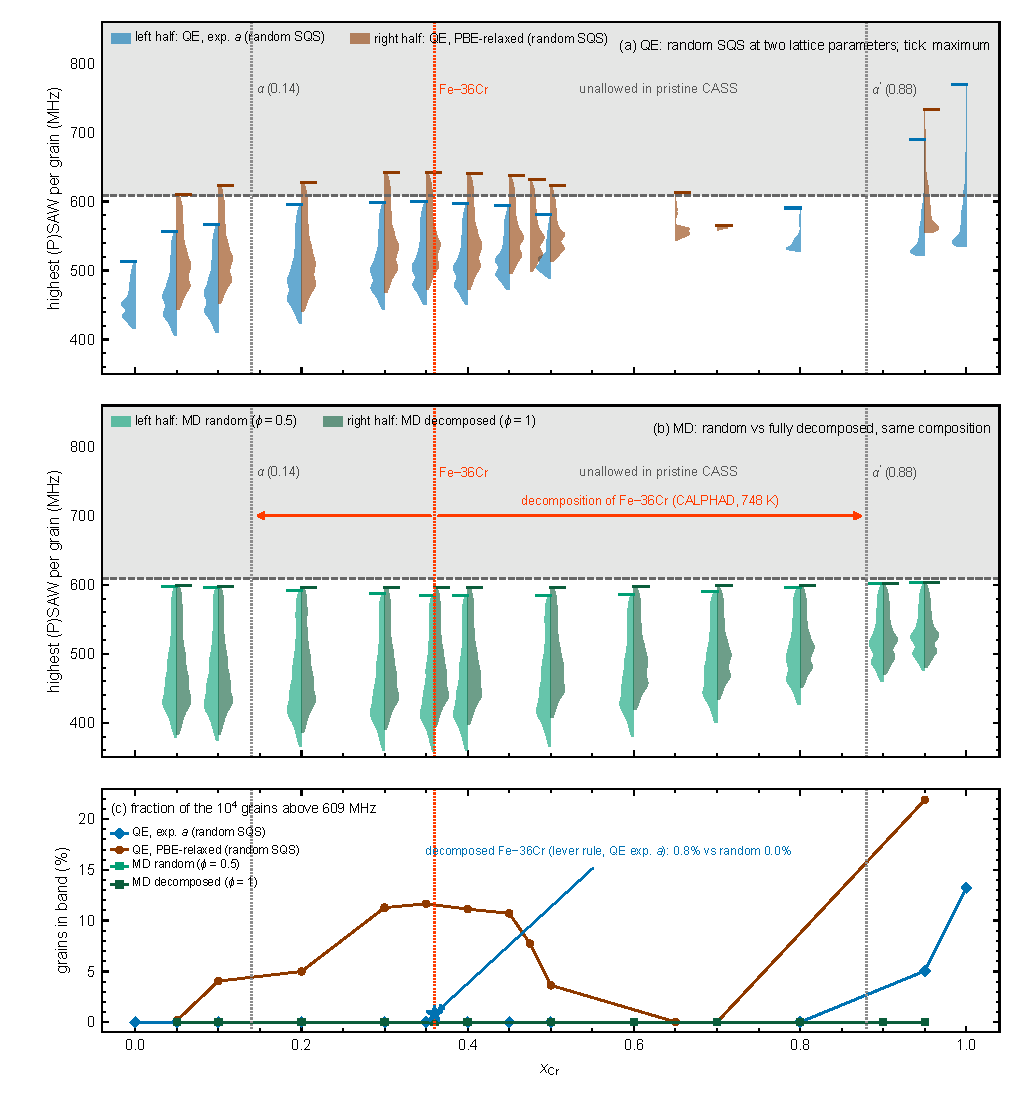
\includegraphics[width=0.95\textwidth]{figures/kdense_scripta/supplementary/S_saw_landscape_v2.pdf}
\caption{Where in composition the surface waves of Fe--Cr reach the band that pristine CASS cannot produce ($>609$~MHz at $\lambda=6.4\,\mu$m), and what decomposition of Fe--36Cr does to it. Split violins show the distribution of the highest (P)SAW frequency of each of $10^4$ randomly oriented grains at each composition (tick: maximum). (a) QE 40-atom SQS, random by construction: experimental lattice parameter (left halves) and PBE-relaxed lattice parameter (right halves). (b) MD $25^3$ cell, tensors averaged over five MD alloys: random, $\phi=0.5$ (left halves) and fully decomposed, $\phi=1$ (right halves) at the same composition. (c) Fraction of grains in the band. Decomposition moves the material of Fe--36Cr to the $\alpha$ and $\alpha'$ compositions (0.14 and 0.88, CALPHAD at 748~K \cite{xiong2011improved}); the lever rule then gives the fraction for decomposed Fe--36Cr (star in c). With the QE tensors at the experimental lattice parameter, the reference set for elastic moduli (Section S8), random alloys stay below the band up to 80\% Cr and the band is reached only on the Cr-rich side (5\% of grains at 95\% Cr, 13\% for AF Cr); decomposed Fe--36Cr has about 0.8\% of grains in the band, all from $\alpha'$, against none as a random alloy. The 80\% Cr tensor, with antiparallel Cr moments and a soft $C_{12}$, stays below the band, so the $\alpha'$ value interpolated at 0.88 (2.7\%) is uncertain. The PBE-relaxed QE tensors reach the band at most compositions (up to 22\%), a consequence of their too-stiff bulk moduli; the classical MD tensors stay below it at every composition, random or decomposed. Scripts: \texttt{scripts/run\_saw\_landscape.py}, \texttt{scripts/make\_saw\_landscape.py}.}
\label{fig:S_saw_landscape}
\end{figure}

\begin{figure}[!htbp]
\centering
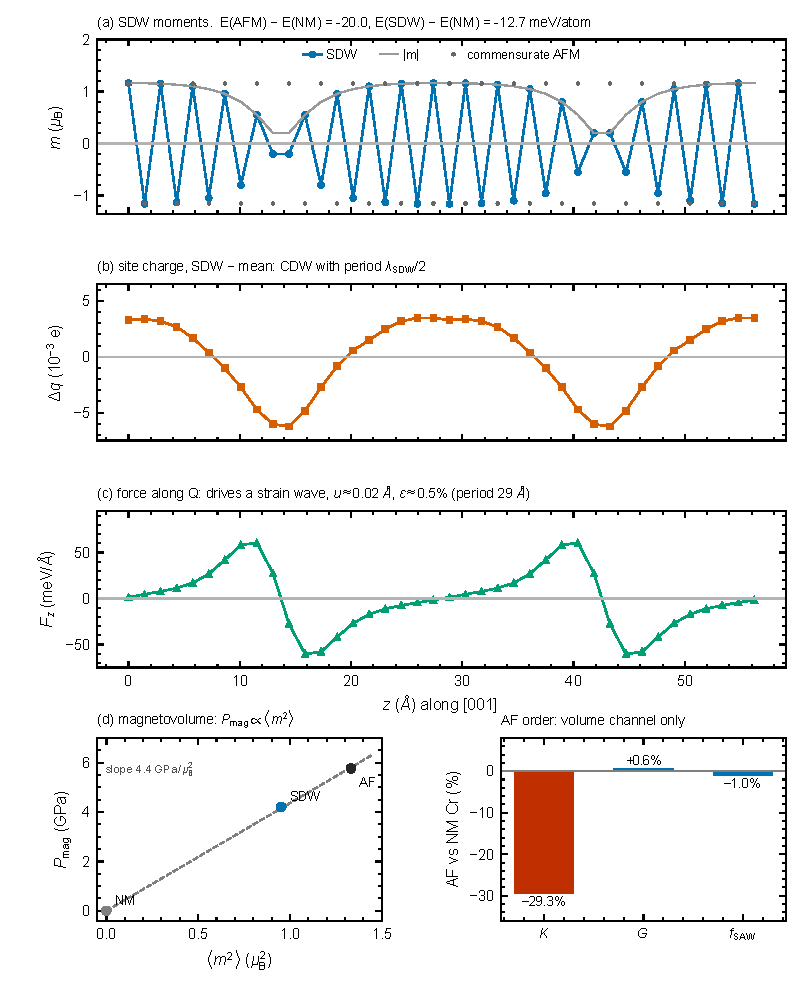
\includegraphics[width=0.66\textwidth]{figures/kdense_scripta/supplementary/S_sdw_cr_v2.pdf}
\caption{Spin- and charge-density wave of \textit{bcc} Cr computed in a $1\times1\times20$ supercell of the conventional cell (40 atoms along [001], room-temperature experimental $a=2.8846$ \AA, $k=16\times16\times1$, other settings as the SQS runs). The supercell sets the incommensurability $\delta=1/20$, close to the measured 0.048 \cite{fawcett1988spin}. (a) Site moments of the SDW, which has nodes every $\lambda_{\mathrm{SDW}}/2=29$ \AA, with the commensurate AFM moments (dots) for comparison. (b) Site charges relative to their mean. They oscillate with period $\lambda_{\mathrm{SDW}}/2$, the charge-density wave that accompanies the SDW, with a peak-to-peak amplitude of about 0.01 e. (c) Forces along $Q$ at the unrelaxed positions, also with period $\lambda_{\mathrm{SDW}}/2$; they drive the strain wave seen by X-ray diffraction \cite{fawcett1988spin}. The static continuum response to their $2\mathbf{Q}$ harmonic, $u=F_{2Q}/(C_{11}\Omega q^2)$, is $u\approx0.02$ \AA\ ($\varepsilon=qu\approx0.5\%$), an upper bound given the PBE moments. (d) From the electrons to the SAW. Left: the magnetic pressure of the AF and SDW cells relative to the non-magnetic one (5.8 and 4.2 GPa) is proportional to $\langle m^2\rangle$ (ratios 0.73 and 0.71), the Landau magnetovolume coupling. Right: in pure Cr (QE, 2-atom cells) AF order lowers $K$ by 29\% but leaves $G$ unchanged ($+0.6\%$), so $f_{\mathrm{SAW}}$ falls by only 1.0\%. Cr magnetism therefore acts on the volume channel, moves the SAW by about 1\%, and its strain wave, with a period of 29 \AA, averages out over the 6.4 $\mu$m TGS wavelength; the $+5\%$ stiffening on decomposition is a shear effect (Fig.~\ref{fig:S_embrittlement}). In PBE the SDW is 12.7 meV/atom below the non-magnetic state but 7.3 meV/atom above the commensurate AFM, and its moments (up to 1.16 $\mu_{\mathrm B}$) exceed the measured 0.62 $\mu_{\mathrm B}$. Both are known shortcomings of semilocal DFT for Cr \cite{hafner2001does,cottenier2002what}, so the figure shows the form of the coupled spin, charge and strain waves, not their measured amplitudes. Script: \texttt{dft\_qe/sdw\_cr.py}.}
\label{fig:S_sdw}
\end{figure}
\clearpage
\begin{figure}[!t]
\centering
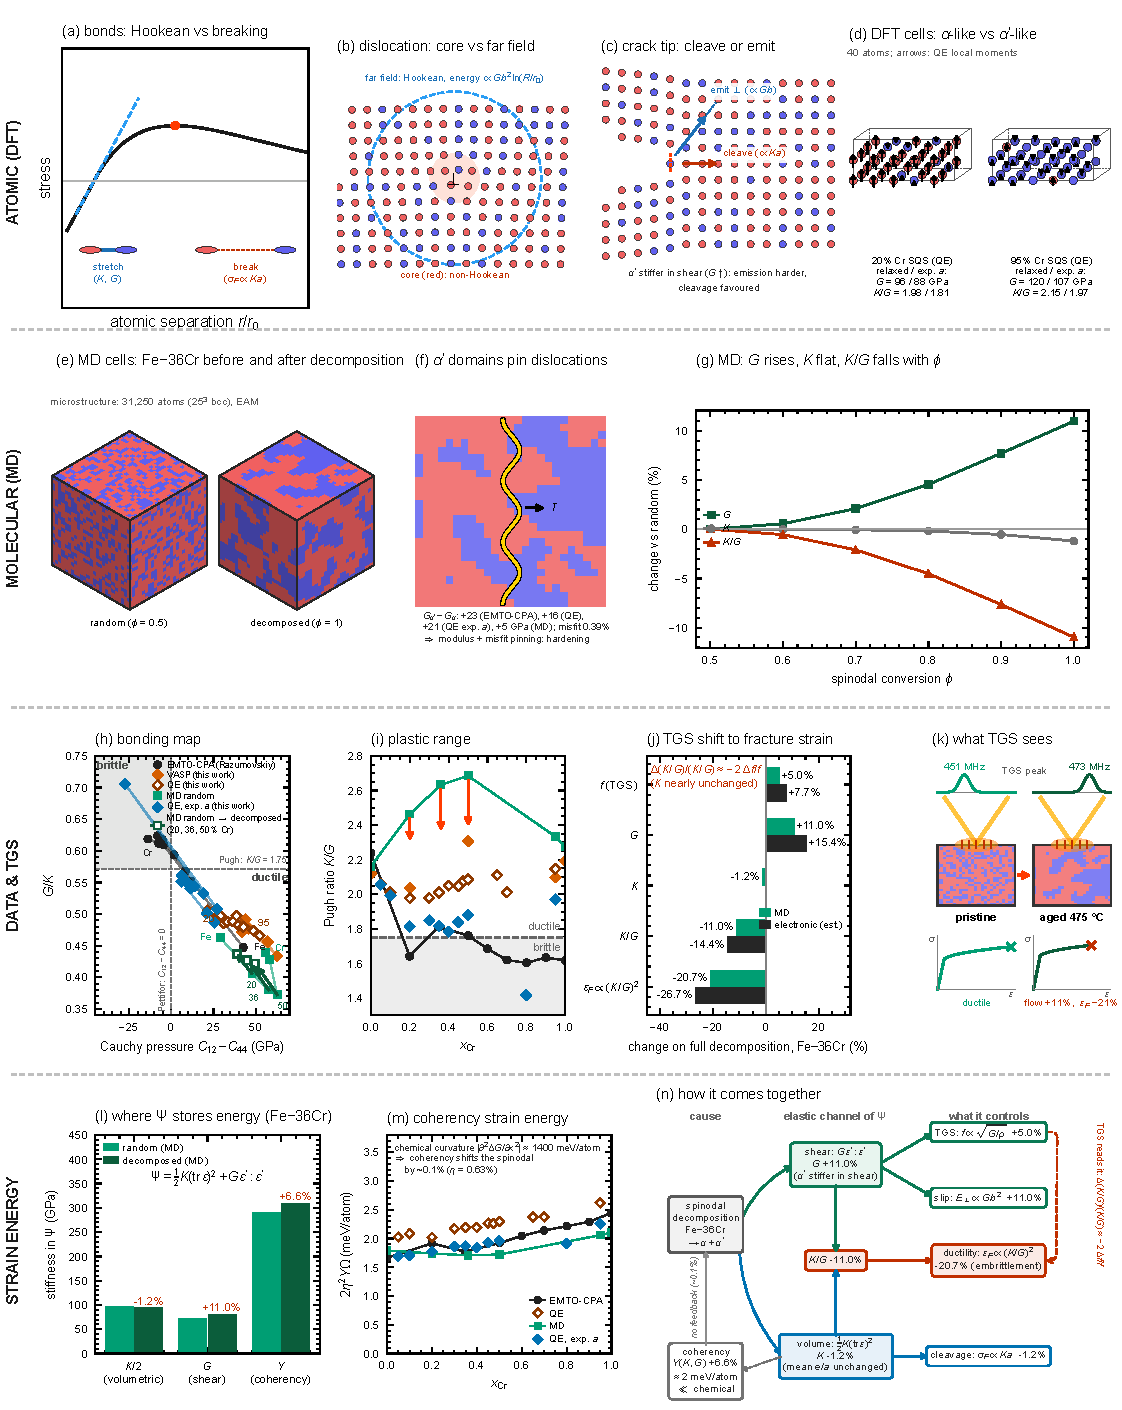
\includegraphics[width=\textwidth,height=0.86\textheight,keepaspectratio]{figures/kdense_scripta/fig5_embrittlement_v7.pdf}
\caption{From elastic stiffening to embrittlement, after Pugh \cite{pugh1954xcii}, at the atomic (DFT) and molecular (MD) scales. Panel descriptions are on the following page.}
\label{fig:S_embrittlement}
\end{figure}


\clearpage
\noindent\textbf{Figure~\ref{fig:S_embrittlement} (continued).} Atomic row (schematic except (d)). (a) A bond stretches in the Hookean regime (slope $\propto K$, and $G$ in shear) and breaks at the non-Hookean peak of the stress--separation curve, so fracture strength scales with $Ka$. (b) An edge dislocation in a random Fe--Cr lattice: its energy, $\propto Gb^2\ln(R/r_0)$, is stored mostly in the Hookean far field, so slip resistance scales with $Gb$. (c) At a crack tip the alloy either cleaves ($\propto Ka$) or emits a dislocation ($\propto Gb$); a phase stiffer in shear makes emission harder and favours cleavage. (d) The relaxed 40-atom QE cells of an $\alpha$-like (20\% Cr) and an $\alpha'$-like (95\% Cr) composition with their local moments: $G$ rises from 96 to 120 GPa (PBE-relaxed; 88 to 107 GPa at the experimental lattice parameter), while their individual $K/G$ (1.98, 2.15; 1.81, 1.97) stays above Pugh's boundary. Molecular row. (e) The $25^3$ MD cells of Fe--36Cr, random ($\phi=0.5$) and fully decomposed ($\phi=1$). (f) A dislocation bowing between $\alpha'$ domains on the decomposed MD plane: the $\alpha/\alpha'$ shear-modulus misfit is $+23$ GPa with the EMTO-CPA moduli, $+16$ and $+21$ GPa with our QE sets (PBE-relaxed, experimental lattice parameter), but about $+5$ GPa with MD, and the lattice misfit is 0.39\%. (g) MD Fe--36Cr: with increasing conversion $\phi$, $G$ rises by 11\%, $K$ stays within 1\% and $K/G$ falls by 11\%. Data and TGS. (h) Bonding map: $G/K$ against the Cauchy pressure $C_{12}-C_{44}$ \cite{pettifor1992theoretical}, each series joined in composition order (labels: at.\% Cr). Dashed lines: Pettifor's ($C_{12}-C_{44}=0$) and Pugh's ($K/G=1.75$) criteria; only the quadrant brittle by both is shaded. EMTO-CPA moves from ductile Fe into that quadrant on the Cr-rich side. Of the tensors of this work, VASP, MD and the PBE-relaxed QE set stay ductile; the QE set at the experimental lattice parameter (filled blue diamonds) approaches Pugh's line between 20 and 50\% Cr ($K/G$ 1.78--1.88) and enters the doubly brittle quadrant at 80\% Cr ($K/G=1.42$, $C_{12}-C_{44}=-28$ GPa), where antiparallel Cr moments soften $C_{12}$ as in AF Cr (Fig.~\ref{fig:S_mechanism}d); the MD paths from random to fully decomposed (20, 36, 50\% Cr; open squares) all point towards brittle without crossing either line. (i) Pugh ratio versus composition, with the empirical ductile/brittle boundary 1.75. (j) Changes on full decomposition of Fe--36Cr: $\Delta(K/G)/(K/G)\approx-2\,\Delta f/f$; with $\varepsilon_F\propto(K/G)^2$ the fracture strain falls by about 21\% (MD) or 27\% (electronic lever-rule estimate). (k) What TGS sees: the peak moves from 451 to 474 MHz while the flow stress rises ($\propto Gb$) and the plastic range shrinks (schematic stress--strain curves). Strain energy (bottom row). The elastic energy density $\Psi(K,G)=\frac12K(\mathrm{tr}\,\varepsilon)^2+G\,\varepsilon':\varepsilon'$ links every step. (l) On decomposition of Fe--36Cr (MD) the volumetric stiffness changes by $-1.2\%$, the shear stiffness by $+11.0\%$ and Cahn's coherency modulus $Y=18KG/(3K+4G)$ by $+6.6\%$. (m) The coherency strain energy $2\eta^2Y\Omega$ is about 2 meV/atom for all tensors ($\eta=0.63\%$), three orders of magnitude below the chemical curvature, so elasticity barely shifts the Fe--Cr spinodal. (n) Mechanism, read left to right: decomposition changes the shear channel of $\Psi$ ($G$ $+11.0\%$; $\alpha'$ is stiffer in shear) but hardly the volume channel ($K$ $-1.2\%$), so $K/G$ falls by 11.0\%. The shear channel sets the TGS frequency ($f=\eta_R(\nu)\sqrt{G/\rho}/\lambda$, $+5.0\%$) and the slip resistance ($\propto Gb^2$, $+11.0\%$); the volume channel sets cleavage ($\propto Ka$, $-1.2\%$); $K/G$ sets ductility ($\varepsilon_F\propto(K/G)^2$, $-20.7\%$). Because $K$ is nearly fixed, the TGS shift reads embrittlement directly, $\Delta(K/G)/(K/G)\approx-2\,\Delta f/f$ (dashed). Coherency ($Y$ $+6.6\%$; about 2 meV/atom against about 1400 meV/atom of chemical curvature) feeds back on the decomposition by only about 0.1\%. Pugh's relations are empirical correlations for pure metals; the numbers indicate direction and scale, not a prediction for CASS.
\clearpage

\subsection*{S10. Spinodal wavelength of the MD structures}
The image analysis of Ref.~\cite{al2023detecting} (Sec.~3.8, Table~4) measured the spinodal wavelength from the Fourier transform of Fe--Cr maps. The same black-and-white maps in three dimensions, measured in real space (chord lengths and the two-point correlation), applied to every decomposed MD structure of this work (12 compositions, five alloys each), is shown in Fig.~\ref{fig:S_spinodal_wavelength}.

\begin{figure}[!htbp]
\centering
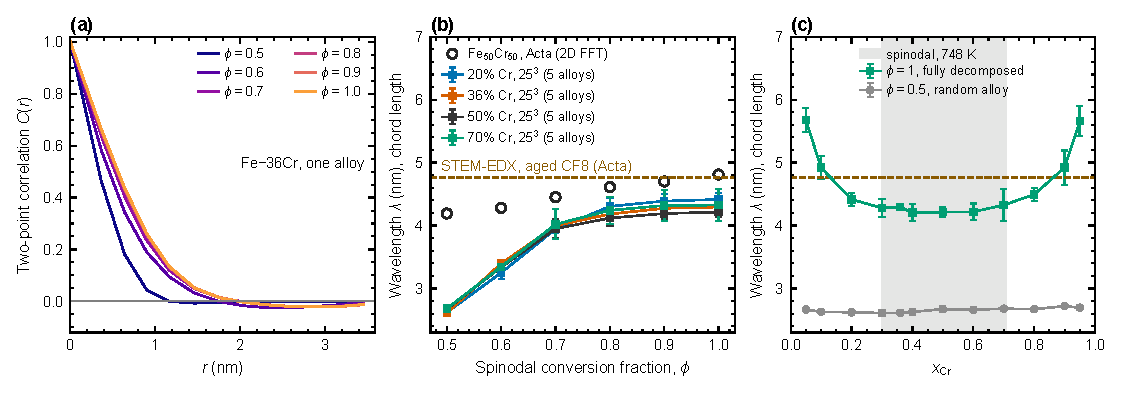
\includegraphics[width=\textwidth]{figures/kdense_scripta/supplementary/S_spinodal_wavelength.pdf}
\caption{Spinodal wavelength of the decomposing MD structures. As in the image analysis of Ref.~\cite{al2023detecting}, each structure is turned into a black-and-white Cr map: the $25^3$ cell is coarse-grained onto its conventional cubic cells, smoothed over one cell and thresholded at the alloy composition (Cr-rich or Fe-rich). (a) Two-point correlation $C(r)$ of the map of Fe--36Cr from the random alloy ($\phi=0.5$) to full decomposition ($\phi=1$): the correlated Cr-rich regions grow from about 1 to 2 nm. (b) Wavelength from the chord lengths, $\lambda=\langle l_{\rm Cr}\rangle+\langle l_{\rm Fe}\rangle$ (mean length of the Cr-rich and Fe-rich runs along all lattice lines, i.e.\ one Fe/Cr period), against $\phi$ (mean $\pm$ s.d. of five alloys), with the 2D-FFT values of Ref.~\cite{al2023detecting} for Fe$_{50}$Cr$_{50}$ ($50^3$ cells, open circles) and its STEM-EDX value for CF8 aged at 400~$^\circ$C for 10 kh (dashed, 4.76 nm). (c) $\lambda$ against Cr content at every $\phi$ (colours as in a). The random alloy gives 2.6--2.7 nm at every composition, the scale of the one-cell smoothing and so the floor of the measure. Inside the spinodal window the wavelength grows from there to 3.3 nm at $\phi=0.6$ and 4.2--4.4 nm at $\phi=1$, the trend and scale of Ref.~\cite{al2023detecting} (4.2--4.8 nm) and of the measured 4.76 nm. Outside the window the minority element forms isolated clusters, and the long matrix runs make $\lambda$ larger without a spinodal period. A 3D FFT of the same maps gives a structure factor that keeps rising towards the lowest $k$ the 7.2~nm box allows, so its wavelength is set by the cell size; the chord lengths are not quantised in this way. The conversion procedure (Sec.~\ref{sec:md}) is a Monte Carlo construction, not aging kinetics, so $\phi$ is not a time. Script: \texttt{scripts/spinodal\_wavelength.py}.}
\label{fig:S_spinodal_wavelength}
\end{figure}


\subsection*{S11. Full text of Sections 2--3}

The main text condenses Sections 2--3 to the journal's word limit. Their full text before condensation follows; equation, figure and section numbers refer to the main text.

\paragraph{2.1 Elastodynamic Methods.}

Elastic waves in each homogeneous alloy obey the elastodynamic wave equation \cite{du2017facile}:

\begin{equation*}
    \rho \frac{\partial^2 u_i}{\partial t^2} = C_{ijkl} \frac{\partial^2 u_k}{\partial x_j \partial x_l}
\end{equation*}

where $C_{ijkl}$ are fourth-order stiffness tensor entries indexed by $i,j,k,l=1,2,3$, $\rho$ is density, and $u$ is the displacement field. On its own, Eq.~\ref{eqn:ewe} describes bulk waves in an unbounded medium. The SAW measured by transient grating spectroscopy (TGS), however, is a Rayleigh wave guided by the free surface. It is obtained from Eq.~\ref{eqn:ewe} for a half-space $x_3 \geq 0$ by requiring a traction-free surface, $\sigma_{i3} = C_{i3kl}\,\partial u_k/\partial x_l = 0$ at $x_3=0$, and displacements that decay with depth. Because crystal orientation is not resolved in the present calculations, we solve this surface problem for the isotropic Voigt--Reuss--Hill (VRH) average of each elastic tensor (Sec.~\ref{sec:analysis}). The Rayleigh velocity is then $v_R = v_s\sqrt{q}$, where $q$ is the root in $0<q<1$ of
\begin{equation*}
q^3 - 8q^2 + (24-16\beta)q - 16(1-\beta) = 0, \qquad \beta = v_s^2/v_p^2,
\end{equation*}
with $v_s=\sqrt{G/\rho}=\sqrt{E/[2(1+\nu)\rho]}$ and $v_p=\sqrt{(B+4G/3)/\rho}$. In practice we evaluate $v_R=(0.874+0.196\nu-0.042\nu^2-0.055\nu^3)\,v_s$, which reproduces the root of Eq.~\ref{eqn:rayleigh} to within 0.02\% for $0.20\leq\nu\leq0.35$. The SAW frequency is $f_{\mathrm{SAW}} = v_R/\lambda$ with $\lambda = 6.4\,\mu$m, the grating period of our TGS measurements \cite{al2023detecting}. Density is interpolated linearly between \textit{bcc} Fe (7870 kg m$^{-3}$) and Cr (7200 kg m$^{-3}$).

The elastic tensor is calculated using a variable cell relaxation algorithm that consists of a loop over iterative self-consistent field (SCF) calculations while adjusting atomic positions and lattice constants. Elasticity theory relates the strain applied to the unit cell to the resulting calculated stress as an inverse problem, which could be solved using a non-linear solver with prior data as an initial guess vector. Deterministic thermoelastic relationships are also used to calculate elastic tensors from changes in total energy and volume using \textit{ab initio} stress calculations. Both methods are used in a self-consistent fashion to converge to a solution that solves the elasticity inverse problem, $\underline{C}\vec{\epsilon} = \vec{\sigma}$, as follows \cite{timoshenko1951theory, mit1620}:

\begin{equation*}
\begin{bmatrix}
C_{1111} & C_{1122} & C_{1133} & C_{1123} & C_{1113} & C_{1112} \\
 & C_{2222} & C_{2233} & C_{2223} & C_{2213} & C_{2212} \\
 &  & C_{3333} & C_{3323} & C_{3313} & C_{3312} \\
 &  &  & C_{2323} & C_{2313} & C_{2312} \\
 & symm &  &  & C_{1313} & C_{1312} \\
 &  &  &  &  & C_{1212}
\end{bmatrix} \begin{bmatrix}
\epsilon_{11} \\
\epsilon_{22} \\
\epsilon_{33} \\
2\epsilon_{23} \\
2\epsilon_{13} \\
2\epsilon_{12}
\end{bmatrix}  =  \begin{bmatrix}
\sigma_{11} \\
\sigma_{22} \\
\sigma_{33} \\
\sigma_{23} \\
\sigma_{13} \\
\sigma_{12}
\end{bmatrix}
\end{equation*}
or in Voigt notation:
\begin{equation*}
 \begin{bmatrix}
C_{11} & C_{12} & C_{13} & C_{14} & C_{15} & C_{16} \\
 & C_{22} & C_{23} & C_{24} & C_{25} & C_{26} \\
 &  & C_{33} & C_{34} & C_{35} & C_{36} \\
 &  &  & C_{44} & C_{45} & C_{46} \\
 & symm &  &  & C_{55} & C_{56} \\
 &  &  &  &  & C_{66}
\end{bmatrix}  \begin{bmatrix}
\epsilon_{1} \\
\epsilon_{2} \\
\epsilon_{3} \\
\epsilon_{4} \\
\epsilon_{5} \\
\epsilon_{6}
\end{bmatrix}  =  \begin{bmatrix}
\sigma_{1} \\
\sigma_{2} \\
\sigma_{3} \\
\sigma_{4} \\
\sigma_{5} \\
\sigma_{6}
\end{bmatrix}
\end{equation*}

\paragraph{2.2 DFT Methods.}

Material properties are calculated from a self-consistent, non-linear field calculation (Fig.~\ref{fig:SCF-loop}), a variational method that optimizes the charge density and adjusts atomic positions until a threshold in energy minimization is achieved in a simplified ion-core model of atoms and electrons \cite{Schwingenschloegl2004}.

Self-consistent, non-linear field calculation algorithms calculate external potentials with a Poisson equation solver, (Fig.~\ref{fig:SCF-loop}) which depends on simulation geometry, atomic positions of ions, pseudopotentials used for the atoms involved, and other inputs. This external potential is then used as a guess for the electron density with a Schr\"{o}dinger equation solver \cite{giustino2014materials}, which is then used as inputs to a self-consistent field loop that calculates the charge density iteratively to minimize the total energy. The accuracy of this algorithm depends on the cut-off applied to the energy minimization, the charge density, the size of the momentum grid, and other convergence thresholds on the outputs \cite{hung2022quantum, Schwingenschloegl2004, giustino2014materials}.

In order to model the BCC Fe--Cr $\delta$--ferrite solid solution, the special quasirandom structure (SQS) methodology was employed \cite{VandeWalleLiu2013}.
The \texttt{mcsqs} software package within the Alloy Theoretic Automated Toolkit (ATAT) was used in order to generate SQS supercells.
The Vienna \textit{ab initio} Simulation Package (VASP) \cite{kresse1996vasp} was used to perform the density functional theory (DFT) total energy calculations, which were used to derive the elastic properties as well as the enthalpy of mixing.
Spin--polarized DFT calculations were performed on 40--atom SQS supercells employing $\Gamma$--point sampling of reciprocal space along with a 500 eV planewave cutoff energy.
The Projector--Augmented Wave (PAW) method \cite{kresse1999paw} was employed for the ionic pseudopotential, and the Perdew--Burke--Ernzerhof parameterization \cite{pbe1996} of the Generalized Gradient Approximation (GGA) of the exchange--correlation functional. Calculations were performed at $x_{\mathrm{Cr}} = 0$, 0.20, 0.50, 0.95, and 1.00.

\paragraph{2.3 Atomistic simulations of decomposed Fe--Cr.}

The spinodal conversion fraction $\phi$ and the corresponding elastic moduli are taken from our earlier atomistic study \cite{al2023detecting} (Sec.~3.7 and Fig.~8 therein). These simulations were performed with LAMMPS \cite{plimpton1995}, not VASP, and include no electronic structure. A $50\times50\times50$ \textit{bcc} cell (lattice parameter 2.866 \AA) of 250,000 atoms with equiatomic composition was populated randomly and phase-separated by Monte Carlo atom swaps at 10 K (3000 attempts every 50 steps for 40,000 steps). The swaps were driven by a structure-generation pair interaction only: zero for like pairs and a strongly repulsive nearest-neighbour Fe--Cr Lennard-Jones term ($\epsilon=10$ eV). Intermediate states were produced by converting a fraction (10--50\%) of the Fe atoms to Cr and the same fraction of Cr atoms to Fe. After box and ionic relaxation, the elastic constants of each state were calculated by finite deformation (strain $10^{-6}$) with the Fe--Cr two-band embedded-atom-method (EAM) potential of Bonny \textit{et al.} \cite{bonny2011iron}, for ten alloys generated with different random seeds. On this scale, $\phi=0.5$ is the random homogeneous alloy and $\phi=1$ the fully separated structure. Relaxed cell volumes were not retained, so the density is held at the equiatomic value of 7535 kg m$^{-3}$ when these moduli are mapped to $f_{\mathrm{SAW}}$ with Eq.~\ref{eqn:rayleigh}. All LAMMPS inputs, random seeds, and potential files are provided in the accompanying repository. For direct comparison with the homogeneous-alloy DFT and literature data, we also computed random (homogeneous) \textit{bcc} alloys at $x_{\mathrm{Cr}}=0$, 0.20, 0.50, 0.95, and 1.00 with the same stiffness procedure, cell, and potential, using ten random seeds for each mixed composition (one for the pure elements), and at $x_{\mathrm{Cr}}=0.10$, 0.30, 0.36, 0.40, 0.60, 0.70, and 0.80 with three seeds each. The random Fe$_{50}$Cr$_{50}$ alloy reproduces the published value ($C_{11}=252.9\pm0.1$ versus $252.7\pm0.1$ GPa), and the seed-to-seed scatter in $C_{11}$ is at most 0.25 GPa. The decomposition procedure was repeated in a $25\times25\times25$ cell (31,250 atoms) at twelve compositions, $x_{\mathrm{Cr}}=0.05$--0.95, for five alloys (random seeds) at each; we report the mean over the five alloys, and the seed-to-seed standard deviation of the stiffening on decomposition is at most 0.1 percentage points. These runs use the current NIST release of the Bonny \textit{et al.} potential files, which are numerically identical to those used in Ref.~\cite{al2023detecting} apart from two format corrections required by current LAMMPS versions: zero-filled pair tables in the s-band file and finite values at $r=0$.

To extend the decomposition series beyond the equiatomic alloy, we repeated the full procedure at twelve compositions from $x_{\mathrm{Cr}}=0.05$ to 0.95 in a $25\times25\times25$ cell (31,250 atoms) with the same number of attempted swaps per atom. Away from 50/50, converting equal fractions of the Fe and Cr atoms changes the overall composition. We therefore converted a fraction $c$ of the Cr atoms and a fraction $cN_{\mathrm{Cr}}/N_{\mathrm{Fe}}$ of the Fe atoms, with $c=2(1-x_{\mathrm{Cr}})(1-\phi)$; this preserves the composition (to within 0.004 in all structures) and is identical to the original procedure at 50/50. Five alloys with different random seeds were generated per composition, and the figures show their mean and standard deviation. As a check, the same small-cell procedure at 50/50 reproduces the bulk modulus of the original series to within 0.2 GPa at every $\phi$, and its fully decomposed $C_{11}$ to within 0.3 GPa (SM Fig.~\ref{fig:S_md_validation}).

\paragraph{3.1 Spinodal stability from demixing free-energy curvature.}

The local stability of a binary solid solution is governed by the curvature of its free energy of mixing with respect to composition. Where $\partial^2 \Delta G_{\mathrm{mix}}/\partial x_{\mathrm{Cr}}^2 < 0$, infinitesimal composition fluctuations lower the free energy, and demixing proceeds spontaneously without the need for nucleation barriers. Figure~\ref{fig:free_energy} is evaluated at 298.15 K from the concentration-dependent interaction models that Levesque \textit{et al.} fitted to PWSCF--PAW and SIESTA--NC calculations \cite{levesque2011simple}, $\Omega(x)=(x-a)(bx^2+cx+d)$, together with the ideal configurational entropy $S_{\mathrm{mix}}$. Following the sign convention of that model, we plot the demixing free energy
\begin{equation*}
\Delta G_{\mathrm{demix}} = \Omega(x)\,x(1-x) + T S_{\mathrm{mix}} = -\Delta G_{\mathrm{mix}}.
\end{equation*}
The spinodal criterion $\partial^2 \Delta G_{\mathrm{mix}}/\partial x_{\mathrm{Cr}}^2 < 0$ therefore appears as \emph{positive} curvature, $\partial^2 \Delta G_{\mathrm{demix}}/\partial x_{\mathrm{Cr}}^2 > 0$, in Fig.~\ref{fig:free_energy}b. Figure~\ref{fig:free_energy}b compares three estimates of this curvature for the PWSCF--PAW model: the exact analytic second derivative, three-point numerical second differences of its tabulated values on the non-uniform composition grid, and a cruder two-point scheme together with a quadratic fit to its values. The three-point values fall on the exact curve. The two-point scheme distorts the magnitudes on the uneven grid, most strongly at $x_{\mathrm{Cr}}=0.70$, next to a duplicated composition in the tabulation, but agrees on where the instability begins.

Figure~\ref{fig:free_energy}b shows that the homogeneous alloy is unstable for $0.21 \lesssim x_{\mathrm{Cr}} \lesssim 0.75$ in the PWSCF--PAW model (with a second, narrow window at $0.87$--$0.98$); the SIESTA--NC model gives $0.25 \lesssim x_{\mathrm{Cr}} \lesssim 0.99$. Both windows contain the Fe--36Cr alloy in which spinodal decomposition was recently detected through TGS stiffening \cite{rae2026tgs}. Because the entropic term lowers the curvature in proportion to $T$, these windows narrow at the higher temperatures used for aging. At 748 K (475\,$^\circ$C) the CALPHAD assessment of Xiong \textit{et al.}, validated by heat capacity, Curie temperatures and atom-probe tomography, places the chemical spinodal at $x_{\mathrm{Cr}}\approx0.30$--0.71 within a miscibility gap of $\approx0.14$--0.88 \cite{xiong2011improved}. Fe--36Cr therefore lies inside the chemical spinodal at the aging temperature, close to its Fe-rich edge, consistent with their observation at 773 K that 37.8 at.\% Cr decomposes spinodally whereas 26.7 at.\% Cr decomposes by nucleation \cite{xiong2011improved}. Within them, elastic and acoustic properties cannot be interpreted assuming a homogeneous solid solution. Instead, any observable elastic response must be understood as emerging from a system that is intrinsically driven toward compositional modulation, providing the foundation for linking free-energy curvature to stiffness evolution and ultimately to ultrasonic observables.

\paragraph{3.2 Elastic stiffening and elastodynamic mapping to Rayleigh SAW observables.}

To connect thermodynamic instability to experimentally measurable quantities, we compute the cubic elastic tensor across $x_{\mathrm{Cr}}$ and propagate these elastic inputs through the surface boundary-value problem of Sec.~2.1. Although $f_{\mathrm{SAW}}$ depends on the full tensor through $B$ and $G$, we use the longitudinal stiffness $C_{11}$ as a compact index of composition-dependent stiffening (Fig.~\ref{fig:elastic_elastodynamics}a). The black circles are literature calculations by Razumovskiy \textit{et al.} \cite{razumovskiy2011first}, the red diamonds are ours, and the green squares are MD (EAM) random alloys computed here with the procedure of our earlier study \cite{al2023detecting}; the open squares are the corresponding fully decomposed structures, which are stiffer than the random alloy at every composition, most strongly at intermediate compositions (e.g., 257.4 versus 247.3 GPa at $x_{\mathrm{Cr}}=0.36$). The present DFT tensors are systematically stiffer than the reference data (e.g., $C_{11}=324$ versus 260 GPa for \textit{bcc} Fe) and correspondingly predict higher frequencies. Possible contributors include the finite SQS size and the magnetic configuration. We therefore interpret relative trends rather than absolute frequencies. Quantum ESPRESSO calculations on 40-atom SQS (SM S3) at the PBE-relaxed lattice parameter (open symbols) match the literature at 20 and 95\% Cr ($f_{\mathrm{SAW}}=0.509$ and 0.591 GHz versus 0.512 and 0.590 GHz) but rise steadily in between. At the experimental lattice parameter used for the literature data (filled blue diamonds), they also follow it between 30 and 50\% Cr ($C_{11}$ within 11 GPa) and level off where the literature $f_{\mathrm{SAW}}$ has its minimum.

As shown in Fig.~\ref{fig:elastic_elastodynamics}, $C_{11}$ depends systematically on chromium concentration (non-monotonically in the literature and DFT data), producing corresponding shifts in the Rayleigh SAW frequency. For a homogeneous solid solution, each composition corresponds to a single tensor, and hence to a single isotropic $f_{\mathrm{SAW}}$ but a distribution of (P)SAW frequencies over grain orientations. In our earlier study, elastodynamic calculations for pristine CASS over randomly sampled grain orientations defined an ``unallowed'' frequency range, above the highest (pseudo-)SAW frequency and below the bulk-wave frequency, in which no surface mode of the pristine material exists; (P)SAW peaks observed there after aging were attributed to stiffened $\delta$-ferrite \cite{al2023detecting}. Figure~\ref{fig:elastic_elastodynamics}b repeats that calculation for every Fe--Cr tensor (10{,}000 grain orientations each, $\lambda=6.4\,\mu$m) \cite{du2017facile}. The bulk waves of all tensors lie above the range ($\geq0.87$ GHz). In the (P)SAW branch, no literature tensor up to $x_{\mathrm{Cr}}=0.7$ and none of the MD tensors reaches it. Full decomposition raises the highest MD (P)SAW frequency, most at intermediate compositions (from 585 to 596 MHz at $x_{\mathrm{Cr}}=0.36$), but not into the range. Only the stiffest tensors enter it: Cr-rich literature alloys (9\% and 29\% of grains above 0.609 GHz at $x_{\mathrm{Cr}}=0.9$ and 1.0) and the present DFT tensors (30\% and 46\% at $x_{\mathrm{Cr}}=0.95$ and 1.0; their systematic overstiffening also places 6--8\% of grains of Fe and Fe$_{50}$Cr$_{50}$ in the range). Frequencies in this range therefore indicate stiffness beyond that of a homogeneous solid solution of $\delta$-ferrite or Fe--36Cr composition, consistent with the stiffer Cr-rich $\alpha'$ regions formed by spinodal decomposition (Fig.~\ref{fig:fsaw_combined}a). This agrees with the mechanism observed experimentally in Ref.~\cite{al2023detecting}, in which aging stiffens the $\delta$-ferrite until its surface-wave peak separates from that of the austenite (peak splitting in 60--100\% of aged spots against 0--25\% unaged; Table~3 of Ref.~\cite{al2023detecting}). Our calculations identify the stiffening that places peaks in the unallowed range: decomposition stiffens mainly the tetragonal shear modulus $C'$ (by 17--29\% for Fe--36Cr, through the Cr-rich $\alpha'$ phase) rather than $C_{44}$, so it cannot lift the top of the (P)SAW branch above about 585~MHz for any microstructure, but it lowers the elastic anisotropy and makes weak high-velocity pseudo-SAWs above 665~MHz, beyond any surface mode of pristine CASS, three to five times more frequent (QE: 0.4 to 1.9\% of grains; EMTO-CPA: 2.6 to 6.2\%), as in the measured tail (0.2\% of peaks above 665~MHz unaged against 2--15\% after aging at 290--400~$^\circ$C; Fig.~9 of Ref.~\cite{al2023detecting}; SM Section S9). At the electronic level, the three effects act on different elastic channels: the stiffer $C'$ of $\alpha'$ follows the filling of the \textit{bcc} $d$ band, which stabilizes the \textit{bcc} lattice towards Cr \cite{soderlind1993theory} (QE: $C'$ rises from 56~GPa at 5\%~Cr to 145~GPa at 95\%~Cr); the electronic topological transition at $x_c\approx0.08$ (SM Section S6) sets the anomalous moduli of the Fe-rich $\alpha$ phase, which decomposition carries across it; and the spin- and charge-density waves of the Cr-rich $\alpha'$ couple to the volume rather than to shear (antiferromagnetic order lowers $K$ of Cr by 29\% but $f_{\mathrm{SAW}}$ by only 1\%; SM Section S9), so they lower $K/G$, Pugh's ductility measure \cite{pugh1954xcii}, without affecting the acoustic signature. The same shear stiffening links the acoustic signal to embrittlement: decomposition raises $G$ (+11\% for MD Fe--36Cr) while leaving $K$ nearly unchanged ($-1.2\%$), so Pugh's ratio $K/G$ falls by 11\% \cite{pugh1954xcii} in step with the SAW shift, $\Delta(K/G)/(K/G)\approx-2\,\Delta f/f$; meanwhile the shear-modulus misfit between $\alpha$ and $\alpha'$ (+16 to +23~GPa from QE and EMTO-CPA) hardens the ferrite against dislocation motion \cite{kato1981hardening}, while the cleavage resistance, which scales with $K$, stays fixed. Stiffening therefore shifts the balance from plastic flow towards cleavage, as in the Charpy energies of Ref.~\cite{al2023detecting}, which fall from 88.5~J to 14--24~J for CF8 aged 10{,}000~h at 330--400~$^\circ$C as the SAW splitting grows from 12 to 128--229~MHz (SM Section S9). These elastic changes act in the regime where Pugh's relations hold \cite{pugh1954xcii}: for metals melting above about 900~$^\circ$C, thermally activated processes play a negligible part in room-temperature plastic deformation, so the stress needed to move a dislocation, and with it the hardness, scales with $Gb$ ($G$, shear modulus; $b$, Burgers vector), while fracture is set by the maximum of the stress--separation curve beyond its Hookean rise and scales with $Ka$ ($K$, bulk modulus; $a$, lattice parameter). Fe--Cr melts above 1500~$^\circ$C, so the shear stiffening on decomposition raises the resistance to dislocation glide, and hence to plastic flow, at an almost unchanged cleavage stress; the Cr-rich $\alpha'$, whose Debye temperature (the elastic scale of the melting point in the Lindemann relation $T_m\propto MV^{2/3}\Theta_D^2$, SM Fig.~S5 \cite{fine1984elastic}) exceeds that of the random alloy by 10--18\% (QE, EMTO-CPA), lies deeper still in this athermal regime, and stiffening and embrittlement therefore advance together. Within the spinodally unstable composition window, elastic stiffening therefore translates into measurable acoustic signatures, enabling stiffness changes to be inferred non-destructively.

\paragraph{3.3 Separating composition trends from spinodal conversion trends.}

While elastic constants vary with chromium concentration even in a homogeneous solid solution, spinodal decomposition introduces an additional, time-dependent microstructural evolution. To disentangle these effects, it is necessary to distinguish changes driven purely by composition from those arising from the progression of phase separation. We therefore report two complementary relationships that isolate these contributions within a unified elastodynamic framework.

Figure~\ref{fig:fsaw_combined}a shows how chromium partitioning produces stiffening. The Fe--36Cr composition lies near a local minimum of the homogeneous $f_{\mathrm{SAW}}(x_{\mathrm{Cr}})$ curve. Spinodal decomposition moves material toward Fe-rich $\alpha$ and Cr-rich $\alpha'$ compositions (arrows); in both directions the homogeneous-alloy frequency increases. The DFT set, with only five compositions, is consistent with this non-monotonic dependence but cannot resolve the minimum. The MD random alloys, an independent classical model, also show a frequency minimum, at $x_{\mathrm{Cr}}\approx0.36$--0.40, i.e.\ at the Fe--36Cr composition, even though their $C_{11}$ increases monotonically (Fig.~\ref{fig:elastic_elastodynamics}a): the minimum comes from the shear moduli, which control the Rayleigh velocity ($C_{44}$ decreases from 116 GPa for Fe to 106 GPa at $x_{\mathrm{Cr}}=0.5$). $C_{11}$ is therefore a convenient index of stiffening, but the SAW response is governed by shear stiffness. Figure~\ref{fig:fsaw_combined}a describes the properties of the constituents; the effective response of the two-phase microstructure additionally depends on phase fractions and on the domain size relative to the SAW wavelength.

Figure~\ref{fig:fsaw_combined}b isolates the effect of decomposition at fixed overall composition. For Fe$_{50}$Cr$_{50}$ in the MD (EAM) simulations, $f_{\mathrm{SAW}}$ increases monotonically from 0.469 GHz for the random alloy ($\phi=0.5$) to 0.490 GHz for the fully separated structure ($\phi=1$), an increase of about 4.6\% under the fixed-density assumption. The empirical-potential and first-principles results therefore agree in sign. Repeating the decomposition at twelve compositions from $x_{\mathrm{Cr}}=0.05$ to 0.95 (Sec.~\ref{sec:md}; Fig.~\ref{fig:fsaw_combined}b) gives frequency increases between the random and fully separated states that are nearly symmetric about the equiatomic composition: 0.5\%, 1.2\%, 2.7\%, 4.3\%, 5.0\%, 5.4\%, and 5.7\% for $x_{\mathrm{Cr}}=0.05$, 0.10, 0.20, 0.30, 0.36, 0.40, and 0.50, and 5.2\%, 4.1\%, 2.7\%, 1.1\%, and 0.4\% for $x_{\mathrm{Cr}}=0.60$, 0.70, 0.80, 0.90, and 0.95 (means over five alloys; standard deviations at most 0.1 percentage points). Stiffening on decomposition is therefore largest within the spinodally unstable window of Fig.~\ref{fig:free_energy}b, including the Fe--36Cr composition, and nearly vanishes for the dilute alloys at either end. The fully separated state is an idealized limit, so these values bound the stiffening from above. At 50/50, the small-cell series lies about 2\% below the original series in absolute frequency because the original moduli used a different isotropic average; the relative changes agree to within about one percentage point. Together, $f_{\mathrm{SAW}}(x_{\mathrm{Cr}})$ captures the baseline elastic response of a homogeneous alloy, and $f_{\mathrm{SAW}}(\phi)$ reflects the additional stiffening associated with progressive spinodal conversion. This separation enables experimental SAW measurements to be interpreted in terms of both composition and decomposition state, providing a pathway to distinguish early-stage spinodal evolution from equilibrium compositional effects.

\end{document}
